\documentclass[11pt,a4paper,titlepage,draft]{article}
\usepackage[utf8]{inputenc}
\usepackage[greek]{babel}
\usepackage{amsmath}
\usepackage{amsfonts}
\usepackage{amssymb}
\usepackage{amsthm}
\usepackage{commath}
\usepackage{xcolor}
\usepackage{hyperref}
\usepackage[skins,theorems]{tcolorbox}
\usepackage{titlesec}
\usepackage{wrapfig}
\usepackage{mathtools}
\usepackage{pgfplots}
\usepackage{subcaption}
\usepackage{float}
\usepackage{relsize}
\usepackage[inline]{enumitem}
\usepackage{cancel}


\usetikzlibrary{arrows.meta}
\usetikzlibrary{calc}
%\usepackage{tkz-euclide} % loads  TikZ and tkz-base
%\usetkzobj{angles} % important you want to use angles

\newlist{enumparen}{enumerate}{1}
\setlist[enumparen]{label=(\arabic*)}

\newlist{enumlatin}{enumerate}{1}
\setlist[enumlatin]{label=(\alph*)}

\usepackage[left=2cm,right=2cm,top=2cm,bottom=2cm]{geometry}

\makeatletter
%\newcommand{\attnboxed}[1]{\textcolor{red}{\fbox{\normalcolor\m@th$\displaystyle#1$}}}
\makeatother
\tcbset{highlight math style={enhanced,colframe=red,colback=white,%
  arc=0pt,boxrule=1pt,shrink tight,boxsep=1.5mm,extrude by=0.5mm}}
\newcommand{\attnboxed}[1]{\tcbhighmath[colback=red!5!white,drop fuzzy shadow,arc=0mm]{#1}}
\titleformat{\section}{\bf\Large}{Κεφάλαιο \thesection}{1em}{}
\newtcolorbox{attnbox}[1]{colback=red!5!white,%
  colframe=red!75!black,fonttitle=\bfseries,title=#1}
\newtcolorbox{infobox}[1]{colback=blue!5!white,%
  colframe=blue!75!black,fonttitle=\bfseries,title=#1}
\newtcolorbox{tbox}[1]{colback=green!5!white,%
  colframe=green!75!black,fonttitle=\bfseries,title=Θεώρημα #1}


\title{Σημειώσεις Λογισμού ΙΙ}
\date{2016, Εαρινό εξάμηνο}
\author{Καναβούρας Κωνσταντίνος \\ \textlatin{\url{http://users.auth.gr/konkanant}}}



\begin{document}

\maketitle

\tableofcontents

\newpage

\part{Ατρέας}

\setcounter{section}{-1}

\begin{itemize}
\item 2 ώρες Ζάχαρης (3.5 μον.)
\item 4 ώρες εγώ (6.5 μον.)

\textlatin{http://users.auth.gr/natreas}
\end{itemize}

\paragraph{}

\begin{itemize}
\item Ρασσιάς Θ.
\item Κωνσταντινίδου Μ.
\item Ξένος
\item Σημειώσεις
\end{itemize}

\section[Διανυσματικές συναρτήσεις \& καμπύλες στο χώρο]{Διανυσματικές συναρτήσεις \\ Καμπύλες στο χώρο}

\paragraph{Ορ.}
Μία συνάρτηση \( \mathbf{r}: A \subseteq \mathbb R \rightarrow \mathbb R ^ n \) απαρτίζεται από:

(α). το πεδίο ορισμού της \(A\) που είναι υποσύνολο της πραγματικής ευθείας και

(β). έναν τύπο έτσι ώστε σε κάθε πραγματικό αριθμό \(t \in A\) αντιστοιχεί \textbf{ΜΟΝΑΔΙΚΟ ΔΙΑΝΥΣΜΑ} \( \mathbf{r}(t) \) στο (διανυσματικό) χώρο \( \mathbb R ^ n \) δηλαδή:

\[
A \subseteq \mathbb R \rightarrow \mathbb R ^ n: \mathbf{r}(t) = \left( f_1(t), \dots, f_n(t) \right)
\]

όπου \(f_1: A \subseteq \mathbb R \rightarrow \mathbb R\) \textbf{συνήθεις} πραγματικές συναρτήσεις.

\paragraph{}
Πεδίο ορισμού διανυσματικής συνάρτησης είναι εκείνο το υποσύνολο του \( \mathbb R \) για όλα τα σημεία του οποίου ο τύπος της συνάρτησης \textbf{ΕΧΕΙ ΝΟΗΜΑ}.

\emph{Πρακτικά}, αν
\[ \mathbf{r}(t) = \left( f_1(t), \dots, f_n(t) \right), \]
τότε το πεδίο ορισμού της \( \mathbf{r} \) προκύπτει από τη \textbf{συναλήθευση} των πεδίων ορισμού ΟΛΩΝ των συναρτήσεων \( f_1,\dots,f_n\).

\emph{π.χ.}
\[ \mathbf r (t) = \left( \ln t, \sqrt{1-t^2} \right) 
\quad \leftarrow \text{διανυσματική συνάρτηση πραγματικής μεταβλητής}
\]
Πρέπει
\[
\begin{cases}
t > 0 \text{ (λόγω λογαρίθμου)} \\
\quad \text{και} \\
1-t^2 > 0 \text{ (λόγω ρίζας)}
\end{cases}
\]
Άρα Π.Ο. της \(\mathbf r\) είναι το \((0,1]\).

\subsubsection{Όριο και συνέχεια διανυσματικών συναρτήσεων}
\paragraph{Θ.} Έστω \(\mathbf r: A \subseteq \mathbb R \rightarrow \mathbb R ^ n\), \( \mathbf r(t) =  \left( f_1(t), \dots, f_n(t) \right) \) διανυσματική συνάρτηση και \(t_0\) είναι σημείο συσσώρευσης (σ.σ.) του \(A\).
Τότε:

\[ \lim _{ t \to t_0 } \mathbf r(t) = \vec{a} = \left( a_1, \dots, a_n \right) \iff
\begin{cases}
 \lim_{ t \to t_0 } f_1(t) = a_1 \\
 \quad \vdots \\
 \lim_{ t \to t_0 } f_n(t) = a_n \\
\end{cases}
\]

Επίσης, αν \(τ_0 \in A\) είναι και σ.σ. του \(Α\), τότε:

\[ \mathbf r \text{ συνεχής στο } τ_0 \iff
f_1,f_2,\dots,f_n  \text{ συνεχείς στο } τ_0
\]

δηλ.
\[ \lim _{ t \to t_0 } \mathbf r(t) = \mathbf r (t_0) \iff
\begin{cases}
 \lim_{ t \to t_0 } f_1(t) = f_1(t_0) \\
 \quad \vdots \\
 \lim_{ t \to t_0 } f_n(t) = f_n(t_0) \\
\end{cases}
\]

\subsection{Καμπύλες στον \(\mathbb R^n\)}
\paragraph{Ορ.}
Έστω \(α,β \in \mathbb R\) με \(α<β\). Κάθε \textbf{ΣΥΝΕΧΗΣ} διανυσματική συνάρτηση:
\[
\mathbf{\gamma}: \attnboxed{[a,b]}
\rightarrow \mathbb R^n: \mathbf r_\gamma(t) = \left( f_1(t),f_2(t),\dots,f_n(t) \right)
\]
καλείται καμπύλη στο χώρο \( \mathbb R ^n \) (και το γράφημά της καλείται ΙΧΝΟΣ της \(\mathbf \gamma\)).


\begin{tikzpicture}
\draw[gray, thick] (-2.5,-2.5) -- (2.5,2.5);
\node[above right, rotate=45] at (-2.5,-2.5) {\(+\infty\)};
\node[above left, rotate=45] at (2.5,2.5) {\(-\infty\)};

\filldraw[black] (0.5,0.5) circle (2pt) node[anchor=west] {\(a\)};

\def\away{7}

\draw[->] (xyz cs:x=\away) -- (xyz cs:x=\away+2.5);
\draw[->] (xyz cs:y=0,x=\away) -- (xyz cs:y=2.5,x=\away);
\draw[->] (xyz cs:z=0,x=\away) -- (xyz cs:z=5,x=\away);

\draw[-{>[scale=2.5,width=3]}, gray] (0.5,0.5) to [bend left=90] (\away+1,3);

\coordinate (A) at (\away+1,2);
\coordinate (B) at (\away+2,1,-0.5);
\coordinate (C) at (\away+3.5,3.5);

\draw [blue, very thick] plot [smooth, tension=2] coordinates { (A) (B) (C) };

\draw[->, very thick] (\away,0) -- (A) node[anchor=east] {\(\mathbf r(a)\)};
\draw[->, very thick] (\away,0) -- (B) node[anchor=west] {\(\mathbf r(t)\)};
\draw[->, very thick] (\away,0) -- (C) node[anchor=east] {\(\mathbf r(b)\)};

\end{tikzpicture}



\subsubsection*{}

Έστω \( \gamma: [a,b] \rightarrow \mathbb R ^ n \) καμπύλη.
\begin{itemize}
\item Η \(\gamma\) θα καλείται \textbf{ΑΠΛΗ} αν είναι 1-1, δηλ. \( \forall t \in (a,b) \) με \(t_1 \neq t_2 \implies \mathbf r(t_1) \neq \mathbf r(t_2)\) (δηλ. ΔΕΝ αυτοτέμνεται).

\item Η \(\gamma\) καλείται \textbf{ΑΝΟΙΚΤΗ}, αν \[\mathbf r(a) \neq \mathbf r(b),\] αλλιώς \textbf{ΚΛΕΙΣΤΗ}.

\item Όλες οι καμπύλες \(\gamma: [a,b] \rightarrow \mathbb R ^ n\) \[\mathbf r_\gamma(t) = \left( f_1(t),f_2(t),\dots,f_n(t) \right)\] λέμε ότι είναι καμπύλες σε \textbf{ΠΑΡΑΜΕΤΡΙΚΗ} μορφή και οι
\(
\begin{cases}
x_1 = f_1(t) \\
x_2 = f_2(t) \\
\quad \vdots \\
x_n = f_n(t)
\end{cases}
\) καλούνται παραμετρικές εξισώσεις της \(\gamma\).

\item Δύο καμπύλες μπορεί να έχουν το \textbf{ΙΔΙΟ ΙΧΝΟΣ}.
\paragraph{π.χ.}
\begin{alignat*}{2}
&\mathbf r_{\gamma_1}(t) = ( \cos t,  && \sin t )  \quad t \in [0, 2 \pi ) \\
&\mathbf r_{\gamma_2}(t) = ( \cos t, - && \sin t )  \quad t \in [0, 2 \pi )
\end{alignat*}
Δηλαδή το ίχνος είναι το ίδιο ΑΛΛΑ αλλάζει η ΦΟΡΑ ΔΙΑΓΡΑΦΗΣ ή ο προσανατολισμός.

\emph{Έτσι}, σε κάθε καμπύλη \(\gamma\) σε παραμετρική μορφή αντιστοιχεί με φυσικό τρόπο ένας \textbf{ΠΡΟΣΑΝΑΤΟΛΙΣΜΟΣ} (ή ΦΟΡΑ ΔΙΑΓΡΑΦΗΣ), πάντα προς την κατεύθυνση αύξησης των \(\gamma\).

\item Έστω \(\gamma_1: [a,b] \rightarrow \mathbb R^n, \gamma_2: [b,c] \rightarrow \mathbb R^n\) καμπύλες.

Καλώ \textbf{ΑΝΤΙΘΕΤΗ} της \(\gamma_1\), συμβολικά \(- \gamma_1\), την καμπύλη που έχει ίδιο ΙΧΝΟΣ με τη \(\gamma_1\) αλλά \textbf{αντίθετη} φορά διαγραφής.

\[ -{\gamma_1} : [a,b] \rightarrow \mathbb R^n : \mathbf r_{-\gamma_1}(t) - \mathbf r_{\gamma_1}(a+b-t)
\]

\item Αν \(\mathbf r_{\gamma_1}(b) = r_{\gamma_2}(b)\), ορίζω την καμπύλη \( \gamma_1+\gamma_2 \) ως εξής:
\[
\gamma_1+\gamma_2: [a,c] \rightarrow \mathbb R^n:
\mathbf r_{\gamma_1+\gamma_2}(t) =
\begin{cases}
\mathbf r_{\gamma_1}, \quad t \in [a,b] \\
\mathbf r_{\gamma_2}, \quad t \in (b, c]
\end{cases}
\]

\item Έστω \( \phi: [c,d] \rightarrow [a,b] \) \textbf{συνεχής} και γνησίως \textbf{μονότονη} συνάρτηση. Τότε η \textbf{σύνθεση}: \[ \mathbf \gamma_1 \circ \phi: [c, d] \rightarrow \mathbb R ^n \]
είναι καμπύλη που καλείται \textbf{ΙΣΟΔΥΝΑΜΗ} της \(\gamma_1\) και έχει το \textbf{ΙΔΙΟ ΙΧΝΟΣ} με τη \(\gamma_1\).

\item Αν \(\phi\) γν. αύξουσα, τότε η σύνθεση έχει και ίδιο προσανατολισμό, αλλιώς αντίθετο προσανατολισμό σε σχέση με τη \(\gamma_1\).
\end{itemize}

\subsection{Παραδείγματα καμπύλων σε παραμετρική μορφή}
\begin{itemize}
\item Έστω \(A,B \in \mathbb R^n\), το \(\overrightarrow{AB}\) παραμετροποιείται ως:
\begin{align*}
\mathbf r(t) &= (\text{αρχή}) + (\text{πέρας}-\text{αρχή}), \quad \attnboxed{t \in [0,1]} \\
&= (a_1, \dots, a_n) + t \left( (b_1, \dots, b_n) - (a_1, \dots, a_n) \right) \\
&= \left( a_1 + t (b_1 - a_1 ), \dots, a_n + t (b_n - a_n) \right), \quad \attnboxed{t \in [0,1]}
\end{align*}
επειδή για κάθε σημείο \(X \in \overrightarrow{AB}\):
\[
\overrightarrow{OX} = \overrightarrow{OA} + \overrightarrow{AX}
= \overrightarrow{OA} + t \overrightarrow{AB}
\]

\item Κύκλος \( (x-a)^2 + (y-b)^2 = R^2\) στο χώρο \(\mathbb R^2\):
\[\mathbf r(t) = \left( f_1(t), f_2(t) \right), \quad t \in [a,b] \quad \leftarrow \text{ παραμετροποίηση γενικά} \]
\emph{Ειδικότερα}
\[
\mathbf r(t) = \left( a+R \cos t, b+ R \sin t \right), \quad t \in [0, 2 \pi)
\]
με θετική φορά διαγραφής (αντιωρολογιακή).

Ή:
\[
\mathbf r(t) = \left( a+R \cos t, b - R \sin t \right), \quad t \in [0, 2 \pi)
\] με αρνητική φορά διαγραφής.

\item Συνάρτηση \(y=f(x)\) πραγματική όπου \(x \in [a,b]\)
\[\mathbf r(t) = \left( x(t), y(t) \right), \quad t \in [a,b] \quad \leftarrow \text{ παραμετροποίηση γενικά} \]
\emph{Ειδικότερα}
\[
\mathbf r(t) = \left( t, f(t) \right) \quad t \in [a, b)
\]

\item Έλλειψη \( \left( \frac{x-a}{A} \right) ^ 2 + \left( \frac{y-b}{B} \right) ^ 2 = 1 \quad \left( \mathbb R^2 \right) \)

\[
\begin{cases}
\frac{x-a}{A} &= \cos t \\
\frac{y-b}{B} &= \sin t
\end{cases}, \text{ τότε}
\begin{cases}
\frac{x}{A} = a+ A \cos{t} \\
\frac{y}{B} = b+ B \sin{t}
\end{cases}
\]
Έτσι \(\mathbf r (t) = (x, y) = (a + A \cos t, b + B \sin t), \quad t \in [0, 2 \pi) \) 

\item Υπερβολή \( \left( \frac{x-a}{A} \right) ^ 2 - \left( \frac{y-b}{B} \right) ^ 2 = 1 \quad \left( \mathbb R^2 \right) \)

\[
\mathbf r (t) = (a + A \cosh t, b + B \sinh t), \quad t \in [0, 2 \pi)
\]

\end{itemize}

\subsection{Παράγωγος διανυσματικών συναρτήσεων μίας μεταβλητής}
\paragraph{Ορ.}
Έστω \(\mathbf r: A \subset \mathbb R \rightarrow  \mathbb R^n : \mathbf r(t) = \left( f_1(t), \dots, f_n(t) \right), \quad t_0 \in A \) είναι σ.σ. του \(Α\). Θα λέμε ότι η \(\mathbf r\) παραγωγίσιμη στο \(t_0\) αν υπάρχει το όριο:
\[
\lim _{t \to t_0} \frac{\mathbf r(t)- \mathbf{r}(t_0)}{t-t_0}
\]
ή ισοδύναμα
\[
\lim _{h \to 0} \frac{\mathbf r(t_0+h)- \mathbf{r}(t_0)}{h}
\]
το οποίο είναι \textbf{ΔΙΑΝΥΣΜΑ} που συμβολίζουμε με \(\mathbf r' (t_0)\) ή \(\frac{\dif \mathbf r}{\dif t}\).

\begin{itemize}
\item Αν η \(\mathbf r\) παραγωγίσιμη σε κάθε σημείο του \(Α\), λέμε ότι είναι παραγωγίσιμη στο \(Α\).
\end{itemize}


\begin{tbox}{}
\(\mathbf{r}\text{ παραγωγίσιμη στο }A \iff f_1,\dots,f_n \text{ παραγ. στο } A\) και
\[
\mathbf r'(t) = \left( f_1'(t),\dots, f_n'(t) \right)
\]
\end{tbox}

\subsubsection{Γεωμετρική ερμηνεία}
Έστω \(h > 0\)

\begin{tikzpicture}
\draw[gray, thick] (-2.5,-2.5) -- (2.5,2.5);
\node[above right, rotate=45] at (-2.5,-2.5) {\(+\infty\)};
\node[above left, rotate=45] at (2.5,2.5) {\(-\infty\)};

\filldraw[black] (0.5,0.5) circle (2pt) node[anchor=west] {\(t_0\)};
\filldraw[black] (-1,-1) circle (2pt) node[anchor=west] {\(t_0+h\)};


\def\away{7}

\draw[->] (xyz cs:x=\away) -- (xyz cs:x=\away+2.5);
\draw[->] (xyz cs:y=0,x=\away) -- (xyz cs:y=2.5,x=\away);
\draw[->] (xyz cs:z=0,x=\away) -- (xyz cs:z=5,x=\away);

\draw[-{>[scale=2.5,width=3]}, gray] (0.5,0.5) to [bend left=90] (\away+1,3);

\coordinate (A) at (\away+0.2,1);
\coordinate (B) at (\away+1.5,3.2);
\coordinate (C) at (\away+4,4);

\draw [blue, very thick] plot [smooth, tension=1] coordinates { (A) (B) (C) };

%\draw[->, very thick] (\away,0) -- (A) node[anchor=east] {\(\mathbf r(a)\)};
\draw[->, very thick] (\away,0) -- (B) node[anchor=west] {\(\mathbf r(t_0)\)};
\draw[->, very thick] (\away,0) -- (C) node[anchor=east] {\(\mathbf r(t_0+h)\)};

\draw[->] (B) -- (C);


\end{tikzpicture}

Το \( \mathbf r'(t) \) έχει τη διεύθυνση της εφαπτόμενης ευθείας της \( \mathbf r\) στο σημείο \( \mathbf r(τ_0)\) και φορά τη φορά της κίνησης. Μπορεί να αναπαριστά π.χ. την ταχύτητα ενός υλικού σημείου.

\subsubsection[Εξίσωση εφαπτομένης]{Εξίσωση (Διανυσματική) εφαπτόμενης ευθείας καμπύλης \(\gamma: [a,b] \rightarrow  \mathbb R ^n = \left(f_1(t),\dots,f_n(t) \right)\) παραγωγίσιμης στο σημείο \(t_0\)}

{\small Αρκεί να ξέρω σημείο της ευθείας και διάνυσμα παράλληλο στην ευθεία}
\begin{attnbox}{Προσοχή!!!}
\[
 \mathbf r_{\text{εφ}}(t) =  \mathbf r(t_0) + \lambda \cdot  \mathbf r'(t_0), \quad \lambda \in  \mathbb R 
 \]
 \end{attnbox}
 
\subsubsection{Ιδιότητες παραγώγου}
Έστω \( \mathbf r_1, \mathbf r_2:[a,b] \rightarrow  \mathbb R ^n\) παραγωγ. καμπύλες, τότε:

\begin{itemize}
\item \( \big( \mathbf r_1 \cdot  \mathbf r_2 \big) ' (t) =
 \mathbf r_1' \cdot  \mathbf r_2(t) +  \mathbf r_1 \cdot  \mathbf r_2'(t)
 \)
\item \( \big( \mathbf r_1 \times  \mathbf r_2 \big) ' (t) =
 \mathbf r_1' \times  \mathbf r_2(t) +  \mathbf r_1 \times  \mathbf r_2'(t)
 \)
 \item \begin{align*} 
 [ \mathbf r_1, \mathbf r_2, \mathbf r_3 ]'(t) = 
 &[ \mathbf r_1', \mathbf r_2, \mathbf r_3 ] + \\
 &[ \mathbf r_1, \mathbf r_2',\mathbf r_3 ] + \\
 &[ \mathbf r_1, \mathbf r_2, \mathbf r_3' ]
\end{align*}
\end{itemize}

\subsection{}
\begin{infobox}{Πρόταση}
Έστω \( \gamma: [a,b] \rightarrow \mathbb R^n: \mathbf r_\gamma (t) = \left( f_1(t),\dots,f_n(t) \right) \) είναι μια παραγωγίσιμη καμπύλη στο \( [a,b] \). \emph{Τότε}:
\[ \left| \mathbf r_\gamma (t) \right| = c = \text{σταθερά } \forall t \iff
\mathbf r_\gamma (t) \bot \mathbf r'_\gamma (t) \ \forall t \]
\tcblower
\begin{proof}
\begin{align*}
|\mathbf r_\gamma(t)| = c \iff \\
|\mathbf r_\gamma(t)|^2 = c^2 \iff \\
\mathbf r_\gamma (t) \cdot \mathbf r_\gamma (t) = c^2 \iff \\
(\mathbf r_\gamma \cdot \mathbf r_\gamma)'(t) = 0 \iff \\
\mathbf r'_\gamma \cdot \mathbf r_\gamma + \mathbf r_\gamma \cdot \mathbf r'_\gamma = 0
\iff \\
\mathbf r'_\gamma \cdot \mathbf r_\gamma = 0 \iff \\
\mathbf r_\gamma \bot \mathbf r'_\gamma
\end{align*}
%TODO Graph 1
\end{proof}

\vspace{-20pt}

\begin{center}
\begin{tikzpicture}[scale=0.7]
\draw[gray, thick] (-2.5,-2.5) -- (2.5,2.5);
\node[above right, rotate=45] at (-2.5,-2.5) {\(+\infty\)};
\node[above left, rotate=45] at (2.5,2.5) {\(-\infty\)};

\filldraw[black] (0.5,0.5) circle (2pt) node[anchor=west] {\(t_0\)};

%TODO Right angle symbol

\def\away{7}

\draw[-{>[scale=2.5,width=3]}, gray] (0.5,0.5) to [bend left=90] (\away,3);

\draw[dashed] (\away,0) circle (3);

\draw (\away-4.22,0.37) -- (\away-0.58,3.44);
\draw (\away+0.15,3.53) -- (\away+3.69,1.1);

\draw (\away,0) -- (\away-1.93,2.3);
\draw (\away,0) -- (\away+1.78,2.41);


\end{tikzpicture}
\end{center}
\end{infobox}

\subsection{Διαφορικό καμπύλης}
Ορίζω \(\dif   \mathbf r _ \gamma (t) = \mathbf r '_ \gamma (t) \dif t\), \textbf{διάνυσμα} πάνω στην εφαπτόμενη καμπύλη στο σημείο \(t\) και φορά που καθορίζεται από το πρόσημο του \(\dif t\).

%TODO Graph 2

Για \(\dif t \to 0\), δηλ. κοντά στο \(t\) ισχύει:
\[ \mathbf r _\gamma (t+dt) - \mathbf r _\gamma (t) \approx d\mathbf r_\gamma (t) \]


%TODO Graph 3

 testαδφξ

\subsubsection{}
\paragraph{Ορ.}
Έστω \(\gamma: [a,b] \to \mathbb R ^n\) καμπύλη σε παραμετρική μορφή.
\begin{enumerate}
\item Η \(\gamma\) καλείται \textbf{ΟΜΑΛΗ} αν είναι παραγωγίσιμη και \( \mathbf r' _ \gamma \neq \mathbf 0 \ \forall t \)
\item Η \( \gamma \) καλείται \textbf{ΛΕΙΑ} αν είναι ΟΜΑΛΗ και η \( \mathbf r _ \gamma \) είναι \textbf{ΣΥΝΕΧΗΣ} συνάρτηση στο \([a,b]\). Αν η \( \mathbf r '_ \gamma \) είναι τμηματικά συνεχής στο \([a,b]\), τότε η \( \mathbf r _ \gamma \) καλείται τμηματικά λεία.
\end{enumerate}

\paragraph{Ορ.}
Έστω \(\mathbf r:[a,b] \to  \mathbb R ^n: \mathbf r _\gamma(t) = 
\left( f_1(t), \dots, f_n(t) \right) \) είναι μια καμπύλη. Ορίζουμε το ορισμένο ολοκλήρωμα της \(\mathbf r_\gamma\) ως εξής:
\[
\underbrace{\int _a^b  \mathbf r _\gamma (t) \dif t}_{\text{διάνυσμα στον }\mathbb R^n}
=
\left(
\int _a^b f_1(t) \dif t + \int _a^b f_2(t) \dif t + \dots
+ \int _a^b f_n(t) \dif t
\right)
\]

Επίσης, υπάρχει παραγωγίσιμη καμπύλη \(\mathbf q:[a,b] \to  \mathbb R ^n:\)
\[
\mathbf q'(t) = \mathbf r_\gamma(t) \quad \forall t
\]
Η \(\mathbf q\) καλείται αντιπαράγωγος της \( \gamma \). Το σύνολο \(
 \left\lbrace \mathbf q(t) + \overline{\mathbf c}: \mathbf{q}
 \text { μια αντιπαράγωγος της }  \mathbf r _ \gamma \text{ και } \mathbf c \in  \mathbb R ^n \text{ σταθερά}  \right\rbrace
 \) καλείται ΑΟΡΙΣΤΟ ΟΛΟΚΛΗΡΩΜΑ της \( \mathbf r _ \gamma \), συμβολικά \(
 \int  \mathbf r _ \gamma (t) \dif t \)
 
Πράγματι,
\begin{align*}
\int  \mathbf r _\gamma (t) \dif t 
&= \left( \int f_1(t) \dif t , \int f_2(t) \dif t, \dots, \int f_n(t) \dif t \right) \\
&= \left( q_1(t)+\overbrace{c_1}^{c_1 \in \mathbb R \text{ αυθαίρετη σταθερά}}, q_2(t)+\overbrace{c_2}^{c_2 \in \mathbb R \text{ αυθαίρετη σταθερά}}, \dots, q_n(t)+\overbrace{c_n}^{c_n \in \mathbb R} \right) \\
&= \left( q_1(t), q_2(t), \dots, q_n(t) \right) + (c_1,\dots,c_n) = 
\mathbf q(t) + \underbrace{\mathbf c}_{\text{αυθαίρετο διάνυσμα}} \in \mathbb R^n
\end{align*}

\subsection{Συμπέρασμα}
\begin{attnbox}{}
Η καμπυλότητα και η στρέψη είναι εκτός ύλης
\end{attnbox}

\subsection{Ασκήσεις}
\paragraph{Άσκ. 1}
Αν \(\gamma:[a,b] \to  \mathbb R ^n: \mathbf r^n (t)
= \left( f_1(t),\dots,f_n(t) \right) \) είναι ΟΜΑΛΗ καμπύλη, ΝΔΟ:
\[
\mathbf r_\gamma (t) \cdot \mathbf r' _\gamma(t) = |\mathbf r _\gamma (t)| \cdot
\left( |\mathbf r_\gamma(t)| \right)'
\]
\begin{proof}
\begin{align*}
 \mathbf r_\gamma(t) \cdot   \mathbf r'_\gamma(t)
 &= \left( f_1(t),\dots ,f_n(t) \right) \cdot \left( f_1'(t),\dots,f'_n(t) \right) \\
&= f_1(t)f'_1(t)+f_2(t)f'2(t)+\dots+f_n(t)f'_n(t)
\end{align*}
\begin{align*}
 |\mathbf r _\gamma (t)| \cdot \left( |\mathbf r_\gamma(t)| \right)'
 &= \sqrt{f_1^2(t) + \dots + f_n^2(t)} + \left( \sqrt{f_1^2(t) + \dots + f_n^2(t)} \right)' \\
 &= \sqrt{f_1^2(t) + \dots + f_n^2(t)} + \frac{1}{2} \frac{2f_1(t)f'1(t)+\dots+2f_n(t)=f'_n(t)}{\sqrt{f_1^2(t) + \dots + f_n^2(t)}} \\
 &= f_1(t)f'_1(t)+f_2(t)f'2(t)+\dots+f_n(t)f'_n(t)
\end{align*}
\end{proof}

\paragraph{Άσκ. 2}
Αν \( \mathbf r_\gamma(t) = t \mathbf i+2 \mathbf j + (t^2-3) \mathbf \kappa\), υπολογίστε την εξίσωση της εφαπτόμενης ευθείας της καμπύλης στο σημείο \((2,2,1)\).
\begin{proof}[Απάντηση]
\[
\begin{cases}
\mathbf i &= (1,0,0) \\
\mathbf j &= (0,1,0) \\
\mathbf \kappa &= (0,0,1) \\
\end{cases}
\]
\[ \mathbf r_\gamma(t) = \left( t,2,t^2-3 \right) \]
\begin{align*}
\mathbf r_\text{εφ}(t) &= 
\left( \text{σημείο ευθείας γνωστό} \right) +
t \left( \text{διάνυσμα παράλληλο στην ευθεία} \right), \quad & t \in  \mathbb R 
\end{align*}
\begin{itemize}
\item Γνωστό σημείο το \(M=(2,2,1)\). Έτσι
\((2,2,1) = (t,2,t^2-3) \implies
\begin{cases}
t&=2\\2&=2\\t^2-3&=1
\end{cases}
\implies t=2
\)
\item Διάνυσμα γνωστό παράλληλο στην εφαπτομένη στο \((2,2,1)\) είναι το
\( \mathbf r'_\gamma(2)\).
\begin{align*}
 \mathbf r'_\gamma(t) &= (1,0,2t) \\
 \mathbf r'_\gamma(2) &= (1,0,4)
\end{align*}
και τελικά:
\begin{align*}
\boxed{
\mathbf r_\text{εφ}(t) = (2,2,1) + t(1,0,4), \quad t \in \mathbb R
}\\
\text{διανυσματική εξίσωση εφαπτόμενης ευθείας}
\end{align*}
\end{itemize}

\end{proof}

\paragraph{Ασκ. 3}[Απάντηση]
Αν \(\mathbf v(t) = \left( 2 \cos t, -t \sin (t^2), 2t \right) \) είναι η ταχύτητα του υλικού σημείου, βρείτε την εξίσωση κίνησης \(\mathbf r_\gamma \), αν \( \mathbf r_\gamma (0) = \mathbf i + 3 \mathbf k\)
\begin{proof}
Είναι γνωστό ότι \(\mathbf v(t) = \mathbf r'_\gamma(t) \implies \int \mathbf r'_\gamma(t) \dif t = \int \mathbf v(t) \dif t \implies \mathbf r_\gamma(t) = \int \mathbf v(t) \dif t = \left( \int 2 \cos t \dif t, \int - t \sin (t^2) \dif t, \int 2t \dif t \right) = \left( 2 \sin t+ c_1, \frac{\cos (t^2)}{2} + c_2, t^2+c_3 \right)\), όπου \(c_1,c_2,c_3 \in \mathbb R \) αυθαίρετες σταθερές (ΑΝΕΞΑΡΤΗΤΕΣ μεταξύ τους).

\[
(1,0,3) \overset{\text{υποθ.}}{=}  \mathbf r_\gamma(0) = 
\left( c_1, \frac{1}{2} + c_2, c_3 \right) \implies
\begin{cases}
c_1&=1 \\
c_2+\frac{1}{2}&=0 \\
c_3&=3
\end{cases}
\implies
\begin{cases}
c_1&=1 \\
c_2&=-\frac{1}{2}=0 \\
c_3&=3
\end{cases}
\]

Τελικά:
\[
\mathbf r_\gamma(t) = 
\left(
2 \sin t +1, \frac{\cos (t^2)-1}{2}, t^2+3
\right)
\]

\end{proof}


\paragraph{Άσκ. 4}
Να παραμετροποιηθούν οι καμπύλες:
\begin{enumerate}
\item \( \left\lbrace \underbrace{x^2+z^2=a^2}_{\text{άπειρος κύλινδρος}}, \ \underbrace{2x+3y+7=1}_{\text{επίπεδο}}  \right\rbrace\)
\item \( \left\lbrace \underbrace{x^2+y^2+z^2=a^2}_{\text{σφαίρα}}, \ \underbrace{2x+3y+z =1}_\text{επίπεδο} \right\rbrace \)
\end{enumerate}

\begin{proof}[Απάντηση]

\begin{enumerate}
\item Η καμπύλη προκύπτει ως τομή "άπειρου" κυλίνδρου \(x^2+z^2=a^2\) και επιπέδου \(2x+3y+z=1\).
%TODO Graph 4p
\begin{infobox}{Παραμετροποίηση καμπύλης}
Γενικά:
\[
\mathbf r_\gamma(t) = \left( x(t), y(t), z(t) \right), \quad t \in [a,b]
\]
\end{infobox}
\[
 \underbrace{\mathbf r_\text{προβολής}(t)}_{\mathclap{\text{πάντοτε είναι ο κύκλος } 
  \left\lbrace x^2+z^2=a^2,y=0  \right\rbrace}} = \left( x(t), 0 , z(t) \right)
\]
Αλλά ο κύκλος \( \left\lbrace  x^2+z^2=a^2,y=0  \right\rbrace \) μπορεί να παραμετροποιηθεί ως εξής:
\[\mathbf r_\text{προβολής}(t) = \left( a \cos t, 0 , a \sin t \right), \quad t \in [0, 2\pi)\]
Έτσι
\[
 \mathbf r_\gamma(t) = \left( a \cos t, y(t), a \sin t \right), t \in [0, 2\pi)
\]
όπου \(2x+3y+z=1 \implies y = \frac{1-z-2x}{3} = \frac{1-a \sin t -2 a \cos t}{3}\).

Τελικά:
\[
 \mathbf r_\gamma(t) = \left( a \cos t, \frac{1-a \sin t - 2 a \cos t}{3}, a \sin t \right), \quad t \in [0, 2\pi)
\]


\item 
\end{enumerate}

Έχουμε \textbf{ΤΟΜΗ} σφαίρας και επιπέδου που είναι \textbf{ΠΑΝΤΑ κύκλος}.

%TODO Graph 5
Θέτω \(z=t\), οπότε \(x^2+y^2=a^2-t^2\), \(y=2x\), \(x^2=\frac{a^2-t^2}{5}\) και προχωρώ λύνοντας \(2 \times 2\) σύστημα

\emph{ή}

\[
\begin{cases}
x^2+y^2+z^2&=a^2 \\
y&=2x
\end{cases}
\iff
\begin{cases}
x^2+(2x)^2+z^2&=a^2 \\
y&=2x
\end{cases}
\iff
\begin{cases}
5x^2+z^2&=a^2 \\
y&=2x
\end{cases}
\]
Οι παραστάσεις είναι ισοδύναμες, δηλαδή η καμπύλη εκφράζεται ως τομή κυλίνδρου και επιπέδου, και ανάγομαι στο ερώτημα (α). Έτσι:
\[
 \mathbf r_\gamma(t) = \left( x(t),y(t),z(t) \right), t \in [a,b]
\]
\[
 \underbrace{\mathbf r_\text{προβολής}(t)}_{\mathclap{\text{είναι πάντα η έλλειψη } 
  \left\lbrace 5x^2+z^2=a^2,y=0  \right\rbrace}} = \left( x(t), 0 , z(t) \right)
\]

Άρα:
\[
\mathbf r_\text{προβολής}(t) = \left( \frac{a}{\sqrt{5}} \cos t,0,a \sin t \right),\quad t \in [0,2\pi)
\]
και έτσι
\[
 \mathbf r_\gamma(t) =  \left( \frac{a}{\sqrt{5}} \cos t,y(t),a \sin t \right)
 \] με \(y(t)=2x(t)=\frac{2a}{\sqrt 5} \cos t\)
 
Τελικά:
\[
 \mathbf r_\gamma(t) = \left( \frac{a}{\sqrt 5} \cos t, \frac{2a}{\sqrt 5} \cos t, a \sin t \right), \quad t \in [0, 2\pi)
\]
\end{proof}




\section{Διπλά Ολοκληρώματα}
\begin{attnbox}{}
Όποιος δεν κατάλαβε τα διπλά ολοκληρώματα, ας μην πάει παρακάτω.
\end{attnbox}

Έστω \(f: R \subset  \mathbb R ^2 \to  \mathbb R: \ z = f(x,y)\) είναι μια συνάρτηση δύο μεταβλητών ΦΡΑΓΜΕΝΗ επί της \textbf{ορθογώνιας περιοχής}:
\[R =  \left\lbrace (x,y): a \leq x \leq b, \ c \leq y \leq d  \right\rbrace\]

%TODO Graph 1

\begin{enumparen}
\item
Διαμερίζω το ορθογώνιο \(R\) μέσω διαμέρισης: \[
\Delta = \left( \Delta_x, \Delta_y \right)
\]
όπου \(
\begin{cases}
\Delta_x &=  \left\lbrace a=x_1<x_2< \cdots < x_N = b  \right\rbrace \\
\Delta_y &=   \left\lbrace c=y_1 < y_2 < \cdots < y_N = d  \right\rbrace
\end{cases}
\) σε στοιχειώδη ορθογώνια \(\Omega_{n,\kappa}\) με εβαδόν:
\[ Ε_{n,\kappa } = \left( x_{n+1} - x_n \right) \left( y_{k+1} - y_k \right) \]
\(n=1,\dots,N-1,\ k=1,\dots,M-1\)

\item
Έστω \((\tilde{x_n}, \tilde{y_n}) \in \Omega_{n,\kappa} \) είναι ΤΥΧΑΙΟ σημείο του \(\Omega_{n,\kappa}\). Ορίζω τις τιμές \(f(\widetilde{x_n}, \widetilde{y_n})\).

\item
Ορίζω το \textbf{άθροισμα}:
\[
S_{N,M,f} := 
\sum_{n=1}^{N-1} \sum_{k=1}^{M-1} \underbrace{f(\widetilde{x_n}, \widetilde{y_n}) \cdot E_{n_k}}_{\text{παριστάνει τον "όγκο"}}
 \]
 
\item
Έστω \(|\Delta| = \max  \left\lbrace \delta_{n, \kappa}:
\begin{cases}
n=1,\dots,N_1\\
k=1,\dots,M-1
\end{cases}
  \right\rbrace\)
(όπου 
\(\delta_{n,k}= \sqrt{ \left(x_{n+1} - x_n \right) ^2 +  \left(y_{n+1} - y_n \right) ^2 }\)
είναι το μήκος της διαγωνίου του ορθογωνίου \(\Omega_{n,k}\) ) είναι το ΜΕΓΙΣΤΟ ΠΛΑΤΟΣ της διαμέρισης \(\Delta\). Αν
\[
\lim_{|\Delta | \to 0} S_{\Delta, f} = 
\lim_{|\Delta | \to 0} \sum_{n=1}^{N-1} \sum_{k=1}^{M-1} f(\tilde{x_n}, \tilde{y_n}) \cdot E_{n_k}
= \lambda \in  \mathbb R 
\]
\textbf{ανεξάρτητα} της επιλογής της διαμέρισης \(\Delta\) και ανεξάρτητα της επιλογής των σημείων \( ( \widetilde{x_n},\widetilde{y_n}) \in \Omega_{n, \kappa } \). 

Τότε λέμε ότι η \(f\) είναι ολοκληρώσιμη κατά \textlatin{Riemann} στην ορθογώνια περιοχή \(R\) και γράφουμε:

\[
\mathlarger{\mathlarger{
 \iint_R f(x,y) \dif x \dif y = \lambda \in \mathbb R 
}} 
 \]
\end{enumparen}



Προσεγγιστικά,
\[ \iint_R f(x,y) \dif x \dif y \approx \sum \sum f(x_n, y_k) \left( x_{n+1}-x_n \right) \left( y_{n+1}-y_n \right) \]


\subsection{Γενίκευση ορισμού σε μη ορθογώνια χωρία}
Έστω \(f: T \subset \mathbb R^2 \to \mathbb R\) ΦΡΑΓΜΕΝΗ συνάρτηση πάνω σε \textbf{ΦΡΑΓΜΕΝΟ χωρίο \(T\)} με το \textbf{σύνορο αυτού \(\partial T\)} να είναι σύνολο ΑΜΕΛΕΗΤΟΥ ΕΜΒΑΔΟΥ.

Έστω \(T \subset R\), όπου \(R\) είναι οποιοδήποτε \textbf{ορθογώνιο χωρίο} που καλύπτει το \(T\).

Ορίζω την επέκταση της \(f\) στο ορθογώνιο χωρίο \(R\) ως εξής:
\[
g(x,y) = 
\begin{cases}
f(x,y),&(x,y) \in T \\
0,& (x,y) \in R-T
\end{cases}
\]

Αν η \(g: R \subset \mathbb R^2 \to \mathbb R\) είναι ολοκληρώσιμη επί του \textbf{ορθογωνίου} \(R\), τότε λέμε ότι η \(f\) είναι ολοκληρώσιμη επί του \(T\) και:
\[
\iint_T f(x,y) \dif x \dif y =
\iint_R g(x,y) \dif x \dif y
\]

\begin{attnbox}{Θεώρημα 1}
Έστω \(f:T \in  \mathbb R ^2 \to  \mathbb R \) είναι \boxed{\textbf{συνεχής}} συνάρτηση επί ΦΡΑΓΜΕΝΟΥ χωρίου \(T\) (το σύνορο \(\partial T\) του οποίου είναι σύνορο αμελητέου εμβαδού) \textbf{ΕΚΤΟΣ ΕΝΔΕΧΟΜΕΝΩΣ από ένα σύνολο σημείων αμελητέου εμβαδού}. Τότε η \(f\) είναι ολοκληρώσιμη επί του \(T\).

\paragraph{ΣΗΜΕΙΩΣΗ} Σύνολα αμελητέου εμβαδού:
\begin{enumparen}
\item Το πολύ αριθμήσιμο πλήθος σημείων
\item Τμηματικά λείες καμπύλες πεπερασμένου μήκος (ή το πολύ αριθμήσιμη ένωση τέτοιων)
\end{enumparen}


\end{attnbox}

\begin{infobox}{Αριθμήσιμο σύνολο \(A\)}
Υπάρχει 1-1 αντιστοιχία του συνόλου φυσικών \(\mathbb N\) με το \(A\).
\[
\mathbb N =  \left\lbrace 1,2,3\dots \right\rbrace
\]

\textit{π.χ}
\begin{itemize}
\item Το \([a,b] \subset \mathbb R\) είναι υπεραριθμήσιμο
\item Το \(\mathbb Z\) είναι αριθμήσιμο
\item Το \(\mathbb Q\) είναι αριθμήσιμο
\end{itemize}
\end{infobox}

\textit{π.χ.}
Έστω \( T =  \left\lbrace (x,y): x^2+y^2 \leq 1  \right\rbrace\) (μοναδιαίος κυκλικός δίσκος)

\begin{itemize}
\item \(f:T \to \mathbb{R}: f(x,y)=x^2+x^2y\)

συνεχής στο \(T\), άρα ολοκληρώσιμη
\item \(f:T\to \mathbb R : f(x,y) = \begin{cases}1,&x=y\\3,&T- \left\lbrace (x,x):|x| \leq 1 \right\rbrace \end{cases}\) %TODO Atreas graph 01

ολοκληρώσιμη διότι είναι συνεχής στο δίσκο \(T\) εκτός από ένα σύνολο σημείων αμελητέου εμβαδού (το σύνολο \( \left\lbrace (x,x): |x|<1 \right\rbrace\))

\item \(f(x,y) = \begin{cases}1 \ & (x,y): x,y \text{ ρητός}
\\
0& (x,y): x,y \text{ άρρητος}
\end{cases},\ (x,y) \in [0,1]^2 = [0,1] \times [0,1]
\)

δεν είναι ολοκληρώσιμη
\end{itemize}

\subsection{Ιδιότητες}

Ισχύουν οι γνωστές ιδιότητες του ολοκληρώματος.

Έστω \(f,g: T \in  \mathbb R ^2 \to \mathbb R \) ολοκληρώσιμες σε φραγμένο χωρίο \(T\) (με σύνορο αμελητέου εμβαδού). Τότε:
\begin{enumparen}
\item \(af \pm bg\) ολοκλ. επί του \(T\) και
\[
\iint_T \big( af \pm bg \big) (x,y) \dif x \dif y
=
a\iint_T f(x,y) \dif x \dif y
\pm
b\iint_T g(x,y) \dif x \dif y
\]
\item \(f\cdot g, \ \frac{f}{g} (g \neq 0),\ |f|\) ολοκλ. επί του \(T\) και
\[
\left|
\iint_T f(x,y) \dif x \dif y
\right|
\leq
\iint_T \left| f(x,y) \right| \dif x \dif y
\]
\item Αν \(f(x,y) \leq g(x,y) \  \forall (x,y)\), τότε:
\[
\iint_T f(x,y) \dif x \dif y
\leq
\iint_T g(x,y) \dif x \dif y
\]
\item Αν \(T\) χωρίο αμελητέου εμβαδού, τότε:
\[
\iint_T f(x,y) \dif x \dif y = 0
\]
\item Αν \(T = T_1 \cup T_2\) και \(T_1 \cap T_2 = \emptyset\) (ή σύνολο αμελητέου εμβαδού), τότε:
\[
\iint_T f(x,y) \dif x \dif y = 
\iint_{T_1} f(x,y) +
\iint_{T_2} f(x,y)
\]
\item Αν \(m \leq f(x,y) \leq M\), τότε:
\[
mE(T) \leq \iint_T f(x,y) \dif x \dif y \leq M E(T)
\]
όπου \(E(T) = \) εμβαδόν χωρίου \(T\)
\item
\textbf{Θεώρημα μέσης τιμής:}
Αν \(m \leq f(x,y) \leq M\) και \(g(x,y) \geq 0 \ \forall (x,y) \in T\), τότε υπάρχει \(\mu \in [m,M]\):
\[
\iint_T f(x,y) g(x,y) \dif x \dif y =
\mu \iint_T g(x,y) \dif x \dif y
\]

Αν επιπλέον \(f\) \textbf{συνεχής} επί του \(T\) και το \(T\) \textbf{συνεκτικό}, υπάρχει \((x_0,y_0) \in T\):
\[
\iint_T f(x,y) \dif x \dif y = f(x_0,y_0) \iint_T g(x,y) \dif x \dif y
\]
\end{enumparen}

\subsection{Υπολογισμός (πρακτικός) Διπλών Ολοκληρωμάτων}
\subsubsection{Σε Ορθογώνια Χωρία}
\begin{attnbox}{Θεώρημα 2 (\textlatin{Fubini})}
Έστω \(f: R \subset  \mathbb R ^2 \to  \mathbb R \) συνεχής επί ορθογωνίου χωρίου \(R =  \left\lbrace (x,y): a \leq x \leq b, \ c \leq y \leq d  \right\rbrace\).
Τότε και οι συναρτήσεις \(g(x) = \int_c^d f(x,y) \dif y\) και \(h(y) = \int_a^bf(x,y) \dif x\) είναι συνεχείς επί των \([a,b]\) και \([c,d]\) αντίστοιχα, και:
\[
\iint_R f(x,y) \dif x \dif y =
\int_a^b g(x) \dif x =
\int_c^d h(y) \dif y
\]

Με άλλα λόγια:
\begin{equation} \label{eq:fubini}
\boxed{
\iint_R f(x,y) \dif x \dif y
=
\int_a^b \left(
\int_c^d f(x,y) \dif y
\right) \dif x =
\int_c^d \left(
\int_a^b f(x,y) \dif x
\right) \dif y
}
\end{equation}

\paragraph{Σημείωση}
\begin{enumparen}
\item Ξεκινάω να ολοκληρώνω ως προς όποια μεταβλητή θέλω, ΠΑΝΤΑ ΑΠΟ ΜΕΣΑ ΠΡΟΣ ΤΑ ΕΞΩ.
Κάθε φορά ολοκληρώνω ως προς μία μεταβλητή, ΚΡΑΤΩΝΤΑΣ τις υπόλοιπες ΣΤΑΘΕΡΕΣ.
\end{enumparen}
\end{attnbox}

\paragraph{\textit{π.χ.}}

Ποιο το διπλό ολοκήρωμα της:
\[
f(x,y)=x^2+y^2
\]
επί του χωρίου \(T =  \left\lbrace (x,y): 0 \leq x \leq 1, \ 2 \leq y \leq 3  \right\rbrace\)?

\[
I = 
\underbrace{
\int_2^3
\int_0^1
}_{\mathclap{\text{εξειδίκευση ορίων}}}
(x^2+y^2) \underbrace{\dif x \dif y}_{\mathclap{\text{τυχαία επιλογή}}}
=
\int_2^3 \left. \frac{x^3}{3}+y^2x \right|^1_0 \dif y
=
\int_2^3 \left( \frac{1}{3}+y^2 \right) \dif y
= \frac{1}{3}y + \left. \frac{y^3}{3} \right|_2^3 = \dots
\]

\subsubsection{Σε μη ορθογώνια χωρία}
Έστω \(T \subset  \mathbb R ^2\) ΦΡΑΓΜΕΝΟ χωρίο (με σύνορο αμελητέου εμβαδού). Τότε,
\begin{enumlatin}
\item Το \(T\) καλείται \textbf{κανονικό ως προς \(\mathbf y\)}, αν \(T\) είναι \textbf{συνεκτικό} και \boxed{\text{κάθε}} ευθεία \(\parallel \mathbf{y'y}\) \textbf{ΕΝΤΟΣ του \(\mathbf T\)} τέμνει το σύνορο του \(T\) \textbf{ακριβώς σε ΔΥΟ ΣΗΜΕΙΑ}.
%TODO Graph 01
\item Το \(T\) καλείται \textbf{κανονικό ως προς \(\mathbf x\)}, αν \(T\) είναι \textbf{συνεκτικό} και \boxed{\text{κάθε}} ευθεία \(\parallel \mathbf{x'x}\) \textbf{ΕΝΤΟΣ του \(\mathbf T\)} τέμνει το σύνορο του \(T\) \textbf{ακριβώς σε ΔΥΟ ΣΗΜΕΙΑ}.
\item Το \(T\) καλείται κανονικό αν είναι κανονικό ως προς \(x\) \boxed{ΚΑΙ} ως προς \(y\).
\end{enumlatin}

\begin{itemize}
\item Ένα χωρίο:
\begin{itemize}
\item μπορεί να ΜΗΝ είναι ΚΑΝΟΝΙΚΟ
\item μπορεί να είναι κανονικό ως προς \(y\) αλλά όχι ως προς \(x\), και αντιστρόφως.
\end{itemize}
\item Αν \(T\) μη κανονικό, το σπάω σε ΕΝΩΣΗ κανονικών (ως προς \(x\) ή $y$) χωρίων.
\end{itemize}

\begin{attnbox}{Θεώρημα 3 (\textlatin{Fubini})}
Έστω \(f: T \subset  \mathbb R ^2 \to  \mathbb R \) συνεχής επί φραγμένου χωρίου \(T\) (με σύνορο αμελητέου εμβαδού).
\begin{enumerate}
\item Αν \(T\) είναι κανονικό ως προς \(y\) χωρίο της μορφής:
\[
T =  \left\lbrace (x,y):\ a \leq x \leq b, \ g(x) \leq y \leq h(x)  \right\rbrace
\]
όπου \(g,h: [a,b] \to  \mathbb R \) συνεχείς συναρτήσεις, τότε:
\[
\iint_T f(x,y) \dif x \dif y =
\int_a^b \left(
\int_{g(x)}^{h(x)} f(x,y) \dif y
\right) \dif x
\]
\item Αν \(T\) είναι κανονικό ως προς \(x\) χωρίο της μορφής:
\[
T =  \left\lbrace (x,y):\ c \leq y \leq d, \ \kappa (x) \leq x \leq \lambda(x)  \right\rbrace
\]
όπου \(\kappa,\lambda: [a,b] \to  \mathbb R \) συνεχείς συναρτήσεις, τότε:
\[
\iint_T f(x,y) \dif x \dif y =
\int_c^d \left(
\int_{\kappa(x)}^{\lambda(x)} f(x,y) \dif x
\right) \dif y
\]
\item Αν \(T\) κανονικό, τότε:
\begin{align*}
\iint_T f(x,y)\dif x \dif y
&=
\int_a^b \left(
\int_{g(x)}^{h(x)} f(x,y) \dif y
\right) \dif x \\
&=
\int_c^d \left(
\int_{\kappa(x)}^{\lambda(x)} f(x,y) \dif x
\right) \dif y
\end{align*}
\end{enumerate}
\end{attnbox}

%TODO Graph 03


\subsection{Εφαρμογές διπλού ολοκληρώματος}
\begin{enumparen}

\item
\textbf{ΟΓΚΟΣ}:
Έστω \(
\boxed{f=f(x,y) \geq 0}
\ \forall(x,y) \in T
\),
όπου \(T \in  \mathbb R ^2\) φραγμένο σύνολο με σύνορο αμελητέου εμβαδού. Τότε, αν \(f\) ολοκληρώσιμη επί του \(T\), έχουμε:
\[
V = \iint_T f(x,y) \dif x \dif y
\]
όπου \(V\) είναι ο όγκος του \boxed{\text{στερεού}} μεταξύ της επιφάνειας \(z=f(x,y)\) του χωρίου \(T\) και της κυλινδρικής επιφάνειας με \textbf{οδηγό καμπύλη} την καμπύλη του συνόρου του χωρίου \(T\) και οι γενέτειρες \( \parallel zz'\).

\item
Έστω \(\rho = \rho (x,y)\) είναι συνεχής πυκνότητα μάζας/φορτίου επί φραγμένου χωρίου \(T\) με σύνορο αμελητέου εμβαδού.

Τότε \(\iint_T \rho(x,y) \dif x \dif \phi = \) Συνολική μάζα/φορτίο επί του επιπέδου χωρίου \(T\).

\[
\iint_T \rho(x,y) \dif x \dif y  \approx
\sum_{k=1}^\mu
\sum_{n=1}^M \rho (x_k,y_k) \cdot (x_{k+1}-x_k)(\phi_{k+1}-y_k)
\]

\item
Αν \(f(x,y)=1)\ \forall (x,y) \in T\), όπου \(T\) φραγμένο χωρίο με σύνορο αμελητέου εμβαδού, τότε:
\[
\iint_T 1 \dif x \dif y = \text{Συνολικό εμβαδό του χωρίου }T
\]
\end{enumparen}

\subsection{Αλλαγή μεταβλητής στα διπλά ολοκληρώματα}

\begin{attnbox}{Θεώρημα 4}
Έστω \(\mathbb F:D \subset \mathbb R^2 \to G \subset \mathbb R^2:\)
\[
\mathbb F(u,v) = \left( x(u,v),\ y(u,v) \right)
\]
είναι διανυσματικό πεδίο, παραγωγίσιμο και αντιστρέψιμο, δηλαδή:
\[
\frac{D(x,y)}{D(u,v)}
=
\left|
\begin{matrix}
x_u & x_v \\
y_u & y_v
\end{matrix}
\right| \neq 0\ \forall (u,v) \in D
\]

Αν \(f:G \to  \mathbb R \ f=f(x,y)\) συνεχής επί του \(G\), τότε:
\[
\iint_G f(x,y) \dif x \dif y
=
\iint_D f \left( x(u,v),\ y(u,v) \right)
\left|
\frac{ D(x,y)}{ D(u,v)}
\right|
\dif u \dif v
\]


\end{attnbox}

\paragraph{Εφαρμογή σε πολικές συντεταγμένες}
\begin{gather*}
(x,y) \leftrightarrow (\rho, \theta) \\
x = \rho \cos \theta \\
y = \rho \sin \theta
\end{gather*}
\subparagraph{Τότε}
\[
\frac{D(x,y)}{D(\rho,\theta)}
\overset{x=\rho \cos \theta}
{\underset{y=\rho \sin \theta}{=}}
\left|
\begin{matrix}
x_\rho & x_\theta \\
y_\rho & y_\theta
\end{matrix}
\right| = \left|
\begin{matrix}
\cos\theta & -\rho\sin\theta \\
\sin\theta & \rho\sin\theta
\end{matrix}
\right|
= \rho
\]
\subparagraph{Δηλαδή}
\[
\iint_G f(x,y) \dif x \dif y
=
\iint_D f(\rho\cos\theta, \rho\sin\theta) \rho \dif \rho \dif \theta
\]

Μη γνήσια ολοκληρώματα εκτός ύλης.

\subsection{Ασκήσεις}
\paragraph{Άσκηση 1}

Υπολογίστε το:
\[
\iint_T (x^2y + x \cos y) \dif x \dif y
\]
επί του χωρίου:
\[
T =  \left\lbrace (x,y):0 \leq x \leq 1, \ -\pi \leq y \leq \pi  \right\rbrace
\]

\begin{align*}
I&=
\overbrace{\int_{-\pi}^\pi
\overbrace{\int_0^1
(x^2y+x\cos y)}^{\text{τα }x\text{ με τα }\dif x}
}^{\text{τα }y\text{ με τα }\dif y}
\underbrace{\dif x \dif y}_{\mathclap{\text{το επέλεξα τυχαία}}}
\\ \text{(διαδοχική ολοκλήρωση ΠΑΝΤΑ από μέσα προς τα έξω)} &=
\int_{\pi}^\pi
\left.
\frac{x^3}{3}y
+ \frac{x^2}{2} \cos y
\right|_0^1
\dif y
\\ &=
\int_{\pi}^\pi
\left(
\frac{y}{3} + \frac{\cos y}{2}
\right)
\dif y
\\ &=
\left.
\frac{y^2}{6} +
\frac{\sin y}{2}
\right|_{-\pi}^\pi
\\ &= 0
\end{align*}


\paragraph{Άσκηση 2}
Υπολογίστε το \(\iint_T (x^2+y^2) \dif x\dif y\) επί του κλειστού και φραγμένου χωρίου μεταξύ των καμπύλων \(y=x^2\) και \(x=y^2\).

\subparagraph{(α) Υποτυπώδες σχήμα}
%TODO Atreas Graph 01

\subparagraph{Σημεία τομής}
\[
\begin{cases}
y&=x^2\\
x&=y^2
\end{cases}
\implies
\begin{cases}
y&=y^4\\
x&=y^2
\end{cases}
\implies
\begin{cases}
y(1-y^3)&=0\\
x&=y^4
\end{cases}
\implies
\begin{cases}
y&=0\\
x&=0
\end{cases}
\text{ή}
\begin{cases}
y&=1\\
x&=1
\end{cases}
\]

\subparagraph{(β)}
Το χωρίο \(T\) είναι κανονικό ως προς $y$. Πράγματι, τυχαία ευθεία \(\epsilon \parallel y'y\) \textbf{εισέρχεται στο \(\mathbf T\) μέσω της \boxed{\text{ΣΥΝΑΡΤΗΣΗΣ \(\mathbf{y=x^2}\)}} και εξέρχεται από το \(\mathbf T\) μέσω της \boxed{\text{ΣΥΝΑΡΤΗΣΗΣ \(\mathbf{y=\sqrt{x}}\)}}}.

Τότε το \(T\) γράφεται ως:
\[
T =  \left\lbrace 
(x,y):
0 \leq x \leq 1,\
x^2 \leq y \leq \sqrt{x}
 \right\rbrace
\]

\subparagraph{Έτσι:}
\begin{align*}
I &=\iint_T (x^2+y^2) \dif x \dif y
\\ &=
\int_0^1
\int_{x^2}^{\sqrt{x}}
(x^2+y^2)
\underbrace{
\dif y \dif x
}_{\mathclap{\text{αναγκαστικά διότι έχω θεωρήσει ότι το χωρίο κανονικό ως προς $y$}}}
\\ &=
\int_0^1
\left. x^2y + \frac{y^3}{3} \right|_{x^2}^{\sqrt{x}}
\dif x
\\ &=
\int_0^1
\left( x^\frac{5}{2} 
+ \frac{x^\frac{3}{2}}{3}-x^4 -\frac{x^6}{3} \right)
\dif x
\\ &=
\left.
\frac{2}{7}x^{\frac{7}{2}}
+ \frac{2}{15} x^\frac{5}{2}
- \frac{x^5}{5}
- \frac{x^7}{21}
\right|_0^1
\\ &=
\frac{2}{7} + \frac{2}{15}
- \frac{1}{5}
- \frac{1}{21}
\end{align*}

\paragraph{Άσκηση 3}
Υπολογίστε τον όγκοτου στερεού μεταξύ της επιφάνειας \(z = f(x,y)=1+xy\), και των επιπέδων \(y=0,\ z=0,\ x+y=1,\ y=x \quad (x,y \geq 0)\).

Γνωρίζω ότι
\[
V = \iint_{\underbrace{\boxed{T}}_?} \underbrace{f(x,y)}_{?} \dif x\dif y
\]

\subparagraph{(Α) Υποτυπώδες σχήμα}
%TODO Atreas Graph 01

\subparagraph{(Β) Προς ολοκλήρωση χωρίο}
\[
V=\iint_T (1+xy) \dif x \dif y
\]
Το χωρίο \(T\) είναι κανονικό (δηλ. και ως προς $x$ και ως προς $y$). Θα εργασθώ Επιλέγοντας το χωρίο \(T\) να είναι κανονικό ως προς \(x\).

%TODO Atreas Graph 02
\textbf{Τότε έχω:}
\begin{align*}
V &= \overbrace{\int_0^\frac{1}{2}}^{\mathclap{\text{προβολή του χωρίου $T$ στον άξονα $y'y$}}} \underbrace{\int_{x_\mathrm{min}}^{x_\mathrm{max}} (1+xy) \dif x}_{\mathclap{\text{κανονικό ως προς $x$,\quad μεταβλητά όρια στο εσωτερικό ολοκλήρωμα}}} \dif y \\
&= \int_0^\frac{1}{2} \int_y^{1-y} (1+xy)\dif x \dif y \\
&= \int_0^\frac{1}{2} x  + \left. \frac{x^2}{2} y \right|_y^{1-y} \dif y \\
&= \int_0^\frac{1}{2}(1-y) + \frac{y}{2}(1-y)^2-y-\frac{y^3}{2} \dif y \\
&= \int_0^\frac{1}{2} \left(
1-y+\frac{y}{2}-y^2+\frac{y^3}{2}-y-\frac{y^3}{2}
 \right) \dif y
 \\ &=
 \int_0^\frac{1}{2} \left(
 1-\frac{3}{2}y-y^2
 \right) \dif y
 \\ &= \left.
 y-\frac{3}{4}y^2-\frac{y^3}{3} \right|_0^\frac{1}{2}
 \\ &= \frac{1}{2}-\frac{3}{16}-\frac{1}{24}
 \\ &= \frac{24-9-2}{18} = \frac{13}{48}
\end{align*}

\begin{attnbox}{Σημείωση}
Αν θεωρήσουμε το χωρίο $T$ κανονικό ως προς \(y\), τότε θα είχα:

%TODO Atreas Graph 03

\[
V = \int_0^\frac{1}{2} \int_0^x (1+xy) \dif y \dif x
+ \int_\frac{1}{2}^1 \int_0^{1-x} (1+xy) \dif y \dif x
\]
\end{attnbox}

\paragraph{Άσκηση 4}
Υπολογίστε το διπλό ολοκλήρωμα
\[
I = \int_0^3 \int_y^3 e^{x^2} \dif x \dif y
\]

\subparagraph{(Α)}
Σην άσκηση, όπως είναι γραμμένο το προς ολοκλήρωση χωρίο, έχει θεωρηθεί κανονικό \textbf{ως προς $\mathbf x$}.

\subparagraph{(Β) Ποιό είναι το χωρίο? Σχεδίαση (υποτυπώδης)}
%TODO Atreas Graph 04
Το προς ολοκλήρωση χωρίο είναι το γραμμοσκιασμένο στο σχήμα

\subparagraph{(Γ)}
Θεωρώ το χωρίο αυτό κανονικό ως προς \(y\) (το οποίο ισχύει) και έχω:
\begin{align*}
Ι &= \int_0^3 \int_0^x e^{x^2} \dif y \dif x
\\ &=
\int_0^3 \left. ye^{x^2} \right|_0^x \dif x
\\ &=
\int_0^x xe^{x^2} \dif x
\\ &= \left.
\frac{1}{2}e^{x^2} \right|_0^3
\\ &= \frac{1}{2}\left(
e^2-1
\right)
\end{align*}

\paragraph{Άσκηση 5}
Μετασχηματίστε τα χωρία
\begin{enumparen}
\item \(A =  \left\lbrace (x,y): 1 \leq x^2+y^2 \leq 4 \right\rbrace\)
\item \(B =  \left\lbrace (x,y): 1 \leq x^2+y^2 \leq 18x \right\rbrace\)
\end{enumparen}
σε πολικές συντεταγμένες.

\begin{enumparen}
\item
%TODO Atreas Graph 05
\[
A' =  \left\lbrace  (\rho,\theta): 1 \leq \rho \leq 2,\ 0 \leq \theta \leq 2\pi\right\rbrace
\]
\item
\[
\begin{cases}
x^2+y^2 =1 \qquad & \text{(κύκλος κέντρου $(0,0)$ ακτ. 1} \\
x^2+y^2 =18x \qquad & \text{(κύκλος κέντρου $(9,0)$ ακτ. 9} 
\end{cases}
\]
\[
x^2-18x+y^2=0 \implies
x^2-2\cdot 9 x +9^2-9^2+y^2=0
\implies (x-9)^2+y^2=9^2
\]

Περιγράφω τις συνοριακές καμπύλες
\(
\begin{cases}
x^2+y^2 &=11 \\
x^2+y^2 &=18x  
\end{cases}
\)
σε πολικές συντεταγμένες (\(x=\rho\cos\theta,\ y=\rho\sin\theta\))
\begin{itemize}
\item \(\rho^2=1 \implies \boxed{\rho=1}\)
\item \(\rho^2=18\rho\cos\theta \implies \boxed{\rho =18\cos\theta}\)
\end{itemize}

Λύνω το σύστημα \(
\begin{cases}
\rho &=1 \\
\rho &= 18\cos\theta
\end{cases}
\) (μου δίνει τα κοινά σημεία τομής των δύο κύκλων)
\[
18\cos\theta=1\implies\cos\theta=\frac{1}{18}
\implies \theta = \arccos\left( \frac{1}{18}\right)
\]

\[
A' =  \left\lbrace
(\rho,\theta): 1 \leq \rho \leq 18\cos\theta,\
-\arccos\left( \frac{1}{18}\right) \leq \theta \leq \arccos\left( \frac{1}{18}\right)
 \right\rbrace
\]
\end{enumparen}

\paragraph{Άσκηση 6}
Υπολογίστε το \(\iint_t (x^2+y^2)\dif x \dif y\) επί του δίσκου \(T =  \left\lbrace (x,y): x^2+y^2 \leq 1  \right\rbrace\)

Με μετασχηματισμό σε πολικές συντεταγμένες \textbf{έχουμε}:
\begin{align*}
I &= \iint_T (x^2+y^2)\dif x \dif y \\ &=
\int_0^{2\pi} \int_0^1 \rho^2 \cdot \rho\dif\rho\dif\theta \\
&=
2\pi \cdot \left. \frac{\rho^4}{4} \right|_0^1 \\
&= \frac{\pi}{2}
\end{align*}

Αν δεν χρησιμοποιούσα πολικές συντεταγμένες:
\begin{align*}
I&=\int_{-1}^1 \int_{-\sqrt{1-x^2}}^{\sqrt{1-x^2}} (x^2+y^2) \dif y \dif x
\\ &=
\int_{-1}^1x^2y+\left. \frac{y^3}{3} \right|_{-\sqrt{1-x^2}}^{\sqrt{1-x^2}} \dif x
\\ &=
2 \int_{-1}^1 x^2\sqrt{1-x^2} + \frac{\left(\sqrt{1-x^2}\right)^3}{3}
\\ &=^{x=\sin x}
\int_{-\frac{\pi}{2}}^\frac{\pi}{2} \dif x
\left(
\sin^2 y \cdot \cos y + \frac{\cos y}{3}
\right)^3 \cos y \dif y
\\ &=^{\cos 2y = 2 \cos^2 y -1}_{1-2 \cos^2 y}  \dots
\end{align*}


\paragraph{Άσκηση 7}
Υπολογίστε το \(\iint_T \sqrt{R^2-x^2-y^2}\dif x \dif y\) επί του χωρίου
\(T =  \left\lbrace (x,y): x^2+y^2\leq kx \right\rbrace\) \( (R > 0 )\)

\subparagraph{(Α) Σχήμα}
Έχουμε \(x^2+y^2 \leq Rx \implies x^2-Rx+y^2\leq0\implies
\underbrace{x^2-2\cdot\frac{R}{2}\cdot x + \left(\frac{R}{2}\right)^2}
_{\left(x-\frac{R}{2}\right)^2+y^2 \leq \frac{R^2}{4}}
-\left(\frac{R}{2}\right)^2+y^2\leq0\), κυκλικός δίσκος κέντρου \(
\left(
\frac{R}{2},0
\right)
\) και ακτίνας \(\frac{R}{2}\).

Θα πρέπει να μετασχηματισθεί σε πολικές συντεταγμένες
\[
A= \left\lbrace 
(\rho,\theta): -\frac{\pi}{2} \leq \theta \leq \frac{\pi}{2},\
0 \leq \rho \leq R\cos\theta
 \right\rbrace
\]

Τότε:
\begin{align*}
I &= \int_{-\frac{\pi}{2}}^\frac{\pi}{2}
\int_0^{R\cos\theta}
\sqrt{R^2-\rho^2} \cdot \overbrace{\rho \dif \rho \dif \theta}^{\mathrlap{\text{κατ' ευθείαν μπορώ να κάνω την αλλαγή}}}
\\ &=
-\frac{1}{2}
\int_{-\frac{\pi}{2}}^\frac{\pi}{2}
\int_0^{R\cos\theta}
(R^2-\rho^2)^\frac{1}{2}
\dif(R^2-\rho^2) \dif \theta
\\ &=
-\frac{1}{2}\cdot\frac{2}{3}
\int_{-\frac{\pi}{2}}^\frac{\pi}{2}
\left.
\left(
R^2-\rho^2
\right)^{\frac{3}{2}}
\right|_0^{R\cos\theta} \dif\theta
\\ &=
-\frac{R^3}{3}
\int_{-\frac{\pi}{2}}^\frac{\pi}{2}
|\sin^3\theta|
\\ &=
\frac{R^3\pi}{3}
-\frac{2R^2}{3}
\int_0^\frac{\pi}{2}
\sin^3\theta\dif\theta
\\ &=
\frac{\pi R^3}{3}
+\frac{2R^3}{3}
\int_0^\frac{\pi}{2}
\sin^2\theta \dif (\cos\theta)
\\ &=
\frac{2R^3}{3}
\int_0^\frac{\pi}{2}
\left(
1-\cos^2\theta
\right) \dif \cos\theta + \frac{\pi R^3}{3}
\\ &=
\frac{2R^3}{3}
\left.
\left(
\cos\theta-\frac{\cos^3\theta}{3}
\right)
\right|_0^\frac{\pi}{2}
+ \frac{\pi R^3}{3}
\\ &= \frac{\pi R^3}{3} - \frac{4R^3}{9}
\end{align*}


\begin{attnbox}{}
\[
\int_a^b f\left(g(x)\right)
\underbrace{g'(x)\dif x}_{\dif g(x)}
\]
\end{attnbox}




\paragraph{Άσκηση}
\begin{attnbox}{SOS!}
\end{attnbox}

Υπολογίστε τον όγκο του φραγμένου στερεού μεταξύ των επιφανειών \(\overbrace{z=3x^2}^{\mathclap{\text{κυλινδρική επιφάνεια γιατί λείπει το $y$}}}\) και \(\underbrace{z=4-x^2-y^2}_{\mathclap{\text{παραβολοειδές}}}\)

\subparagraph{(Α) Υποτυπώδες σχήμα}
%TODO Atreas 01
\subparagraph{(Β) Χωρίο ολοκλήρωσης}
Η \textbf{προβολή} της τομής των δύο επιφανειών είναι:
\[
\begin{cases}
z&=3x^2\\z&=4-x^2-y^2
\end{cases}
\implies
3x^4-x^2-y^2\implies 4x^2+y^2=4 \implies x^2+\frac{y^2}{4}=1 \text{ (έλλειψη)}
\]

Άρα ολοκληρώνω εντός του χωρίου \(T\)

\subparagraph{(Γ) Τι ολοκληρώνω?}
\begin{align*}
V &= \iint_T \big(z_\mathrm{max} - z_\mathrm{min}\big)(x,y)\dif x \dif y\\
&= \iint_T (4-x^2-y^2)-3x^2 \dif x \dif y
\end{align*}

\subparagraph{(Δ) Υπολογισμός}
\[
V = \iint_T (4-4x^2-y^2)\dif x \dif y
\]

Θα χρησιμοποιήσω το μετασχηματισμό:
\[
\begin{cases}
x&=\rho\cos\theta\\
y&=2\rho\sin\theta
\end{cases}
\]


\begin{align*}
\left| \frac{D(x,y)}{D(\rho,\theta)} \right| =
\left|
\begin{matrix}
x_\rho&x_\theta\\
y_\rho&y_\theta
\end{matrix}
\right| = \left|
\begin{matrix}
\cos\theta&-\rho\sin\theta\\
2\cos\theta&2\rho\sin\theta
\end{matrix}
\right| = 2\rho
\end{align*}
και
\begin{align*}
x^2+\frac{y^2}{4}=1 \implies^{x=\rho\cos\theta}_{y=2\rho\sin\theta}
\rho^2=1 \implies \boxed{\rho=1}
\end{align*}
άρα το χωρίο \(T\) μετασχηματίζεται στο:
\[
T' =  \left\lbrace 
(\rho,\theta):\ 0\leq\rho\leq1,\ 0\leq\theta\leq2\pi
 \right\rbrace
\]
\textbf{άρα:}
\begin{align*}
V&=\iint_T \left( 4-4x^2-y^2\right)\dif x\dif y\\
&= \iint_{T'} \left( 4-4\rho^2\cos^2\theta-4\rho^2\sin^2\theta\right)
\mathbf{2\rho}\dif\rho\dif\theta\\
&=
8\int_0^{2\pi} \int_0^1 \left(1-\rho^2\right)\rho\dif\rho\dif\theta \\
&= 8\cdot2\pi\cdot \int_0^1 \left(\rho-\rho^3\right)\dif\rho = 4\pi
\end{align*}

\paragraph{Άσκηση}
Υπολογίστε το εμβαδόν μεταξύ των καμπύλων \(\rho=a\sin\theta,\ \rho=a\left(1-\cos\theta\right),\quad a>0\) στο ΑΝΩ ημιεπίπεδο.

\subparagraph{(Α)}
\[
E = \iint_T 1 \dif x \dif y = \iint_{T'} \rho\dif\rho\dif\theta
\]
Εννοείται η άσκηση μπορεί να λυθεί και με τον τύπο του εμβαδού του Λογισμού \textlatin{I}.
%TODO Atreas Graph 03

\textbf{Άρα:}
\begin{itemize}
\item \(a\sin\theta \geq a(1-\cos\theta)\ \forall \theta \in [0,\frac{\pi}{2}]\)
\item \(a\sin\theta\leq a(1-\cos\theta)\ \forall \theta \in [\frac{\pi}{2},\pi]\)
\end{itemize}

\begin{align*}
E=&\int_0^\frac{\pi}{2}\int^{a\sin\theta}_{a(1-\cos\theta)}\rho\dif\rho\dif\theta +
\\
+&\int_\frac{\pi}{2}^\pi\int_{a\sin\theta}^{a(1-\cos\theta)}\rho\dif\rho\dif\theta
\end{align*}


\paragraph{Άσκηση}
Υπολογίστε το \(\iint_D e^{\frac{x-y}{x+y}} \dif x \dif y\) επί του χωρίου του σχήματος:
%TODO Atreas Graph 01

Θα εφαρμόσουμε αλλαγή μεταβλητών:
\[
\begin{cases}
u&=x-y\\v&=x+y
\end{cases}
\implies
\begin{cases}
x&=\frac{u+v}{2}\\
y&=\frac{-u+v}{2}
\end{cases}
\]
άρα
\[
\frac{D(x,y)}{D(u,v)} = \left|
\begin{matrix}
x_u&x_v\\y_u&y_v
\end{matrix}
\right|=\left|
\begin{matrix}
\frac{1}{2}&\frac{1}{2}\\-\frac{1}{2}&\frac{1}{2}
\end{matrix}
\right|=\frac{1}{4}+\frac{1}{4}=\frac{1}{2}
\]

\textbf{Άρα:}
\[
\iint_D e^{\frac{x-y}{x+y}}\dif x \dif y = \iint_\mathbf{D'}e^\frac{u}{v} \cdot \left|
\frac{D(x,y)}{D(u,v)}\right|\dif u \dif v = \iint_{D'} e^\frac{u}{v}\left|\frac{1}{2}\right| \dif u \dif v
= \frac{1}{2} \iint_{D'} e^\frac{u}{v} \dif u \dif v
\]

\subparagraph{Σχεδίαση χωρίου $D'$}
\begin{itemize}
\item \(x+y=1 \implies^{x=\frac{u+v}{2}}_{x=\frac{u+v}{2}} \frac{u+v}{2}+ \frac{-u+v}{2} = 1 \implies \boxed{v=1}\)\\
\item \(x+y=2 \implies \frac{u+v}{2}+ \frac{-u+v}{2} = 2 \implies \boxed{v=2}\)\\
\item \(x=0 \implies \frac{u+v}{2} = 0 \implies \boxed{v=-u}\)
\item \(y=0 \implies \frac{-u+v}{2} = 0 \implies \boxed{v=u}\)
\end{itemize}

\subparagraph{Τελικά}
\begin{align*}
I &= \int_1^2\int_{-v}^v e^\frac{u}{v} \dif u \dif v \\
&= \frac{1}{2} \int_1^2 \left.ve^\frac{u}{v}\right|_{-v}^v \dif v \\
&= \frac{1}{2} \int_1^2 v(e-e^{-1})\dif v \\
&= \frac{1}{4} \left. v^2 \right|_1^2 \cdot \left( e-\frac{1}{e} \right) = \frac{3}{4} \left(
e- \frac{1}{e}
\right)
\end{align*}

%TODO Atreas 03
%TODO Atreas 04



\section{Τριπλά Ολοκληρώματα}
Έστω \(f: R \subset  \mathbb R ^3 \to  \mathbb R \) \textbf{φραγμένη} συνάρτηση επί ορθογωνίου \textbf{παραλληλεπιπέδου}
\[
R =  \left\lbrace (x,y,z): a_1\leq x\leq b_1,\ a_2\leq y\leq b_2,\ a_3\leq z\leq b_3  \right\rbrace
\]
και \(\Delta = (\Delta_x,\Delta_y,\Delta_z)\), όπου \begin{align*}
\Delta_x &=  \left\lbrace a_1=x_0 < x_1 < \dots < x_N = b_1  \right\rbrace \\
\Delta_y &=  \left\lbrace a_2=y_0 < y_1 < \dots < y_N = b_2  \right\rbrace \\
\Delta_z &=  \left\lbrace a_3=z_0 < z_1 < \dots < z_N = b_3  \right\rbrace \\
\end{align*}
διαμέριση του \(R\) σε $Ν\cdot M \cdot K\) "στοιχειώδη" ορθογώνια παραλληλεπίπεδα \(\Omega_{n,m,k}\) όγκου
\[
V_{n,m,k} = (x_{n+1}-x_n)(y_{n+1}-y_n)(z_{n+1}-z_n)
\qquad
\begin{cases}
n&=0,\dots,N-1\\
m&=0,\dots,M-1\\
k&=0,\dots,K-1
\end{cases}
\]

Έστω \((\widetilde{x_n},\widetilde{y_m},\widetilde{z_k})\) είναι τυχαίο σημείο στο ορθογ. παρ/δο \(\Omega_{n,m,k}\) και ορίζω την \(f(\widetilde{x_n},\widetilde{y_m},\widetilde{z_k})\ \forall_{n,m,k}\).

Θεωρώ το άθροισμα:
\[
S(f,\Delta) = \sum_{n=0}^{N-1} \sum_{m=0}^{M-1} \sum_{k=0}^{K-1} f(\widetilde{x_n},\widetilde{y_m},\widetilde{z_k}) V_{n,m,k}
\]

Έστω \(|\Delta| = \max \left\lbrace \delta_{n,m,k}:\ n=0,\dots,N-1,\ m=0,\dots,M-1,\ k=0,\dots,K-1 \right\rbrace\) είναι το πλάτος της έδιαμρισης $\Delta$, όπου:
\[
\delta_{n,m,k} = \max  \left\lbrace |\rho\rho'|:\ \forall \rho,\rho; \in \Omega_{n,m,k} \right\rbrace
\]

Αν \(\lim\limits_{|\Delta|\to0} S(f,\Delta) = \lambda \in \mathbb R\), ανεξάρτητα της διαμέρισης $\Delta$ και της επιλογής των σημείων \((\widetilde{x_n},\widetilde{y_m},\widetilde{z_k}) \in \Omega_{n,m,k}\), τότε λέμε ότι υπάρχει το τριπλό ολοκλήρωμα της \(f\) επί του παραλ/δου \(R\) και γράφουμε:

\[
\iiint_R f(x,y,z) \dif x \dif y \dif z = \lambda \in \mathbb{R}
\]

\paragraph{}

Ο ορισμός γενικεύεται και για κλειστά και φραγμένα στερεά του \( \mathbb R ^3\) ως εξής:

Έστω \(S \subset  \mathbb R ^3 \) κλειστό και φραγμένο στερεό με σύνορο αμελητέου όγκου (π.χ. το σύνορό του αποτελείται από ένωση επιφανειών \(z=f(x,y)\)). Έστω
\[
S \subset \Omega
\]
όπου \(\Omega\) ορθογ. παρ/δο που καλύπτει το \(S\).

Αν $f:S \subset \mathbb R^3 \to  \mathbb R $, ορίζω την επέκτασή της στο \(\Omega\) ως εξής:
\[
g(x,y,z) = \begin{cases}
f(x,y,z),\quad&(x,y,z)\in S\\
0,\quad&(x,y,z)\in \Omega-S
\end{cases}
\]

Αν η \(g:\Omega \subset  \mathbb R ^3\to \mathbb R \) είναι ολοκληρώσιμη επί του \(\Omega\), τότε ορίζουμε:
\[
\iiint_S f(x,y,z)\dif x\dif y\dif z=
\iiint_\Omega g(x,y,z)\dif x\dif y \dif z
\]
και αποδεικνύεται ότι ο ορισμός αυτός \textbf{ΔΕΝ} εξαρτάται απ' την επιλογή του \(\Omega \supset S\).

\begin{attnbox}{Θεώρημα}
Έστω \(f:S\in  \mathbb R ^3\to  \mathbb R \) (όπου $S$ κλειστό και φραγμένο στερεό με σύνορο αμελητέου όγκου) \textbf{ΣΥΝΕΧΗΣ} στο \(S\), \textbf{εκτός ενδεχομένως} από ένα σύνολο σημείων αμελητέου όγκου.

Τότε η \(f\) ολοκληρώσιμη επί του \(S\).
\end{attnbox}

\subsection{Ιδιότητες}
Όπως στα διπλά.

\subsection{Υπολογισμός τριπλών ολοκληρωμάτων}
\paragraph{\boxed{\mathrm A} Σε ορθογώνια παραλ/δα}
\subparagraph{Θ (\textlatin{Fubini})} Έστω \(f:R \subset  \mathbb R ^3\to  \mathbb R \) \textbf{ΣΥΝΕΧΗΣ} επί ορθογ. παρ/δου
\[
R =  \left\lbrace (x,y,z): a_1\leq x\leq b_1,\ a_2\leq y\leq b_2,\ a_3\leq z\leq b_3  \right\rbrace
\]

Έστω \begin{align*}
D_{xy} &= [a_1,b_1]\times[a_2,b_2]\\
D_{yz} &= [a_2,b_2]\times[a_3,b_3]\\
D_{xz} &= [a_1,b_1]\times[a_3,b_3]
\end{align*}
είναι οι ορθογώνιες προβολές του παρ/δου \(R\) στα επίπεδα \(xy,\ yz\) και \(xz\) αντιστοίχως.

Τότε οι συναρτήσεις
\begin{align*}
g(x,y)&=\int_{a_3}^{b_3}f(x,y,z)\dif z,\\
g(y,z)&=\int_{a_1}^{b_1}f(x,y,z)\dif x,\\
g(x,z)&=\int_{a_2}^{b_2}f(x,y,z)\dif y
\end{align*}
είναι \textbf{συνεχείς} επί των προβολών \(D_{xy},D_{yz},D_{xz}\) αντιστοίχως και
\begin{align*}
\iiint_R f(x,y,z)\dif x \dif y \dif z & =
\iint_{D_{xy}} \left(
\int_{a_3}^{b_3} f(x,y,z) \dif z
\right) \dif x \dif y  \qquad
\begin{cases}
\int_{a_1}^{b_1}\int_{a_2}^{b_2}\int_{a_3}^{b_3} \cdots \dif z \dif y \dif x\\
\int_{a_2}^{b_2}\int_{a_1}^{b_1}\int_{a_3}^{b_3} \cdots \dif z \dif x \dif y
\end{cases}
\\
& =
\iint_{D_{yz}} \left(
\int_{a_1}^{b_1} f(x,y,z) \dif x
\right) \dif y \dif z \qquad \begin{cases}
\int_{a_2}^{b_2}\int_{a_3}^{b_3}\int_{a_1}^{b_1} \cdots \dif x \dif z \dif y\\
\int_{a_2}^{b_3}\int_{a_2}^{b_2}\int_{a_1}^{b_1} \cdots \dif x \dif y \dif z
\end{cases}\\
& =
\iint_{D_{xz}} \left(
\int_{a_2}^{b_2} f(x,y,z) \dif z
\right) \dif x \dif y \qquad
\begin{cases}
\int_{a_1}^{b_1}\int_{a_3}^{b_3}\int_{a_2}^{b_2} \cdots \dif y \dif z \dif x\\
\int_{a_3}^{b_3}\int_{a_1}^{b_1}\int_{a_2}^{b_2} \cdots \dif y \dif x \dif z
\end{cases}
\end{align*}

\subparagraph{π.χ.}
Υπολογίστε το \(\iint_S xyz \dif x \dif z \dif y\) επί του στερεού \(S= \left\lbrace (x,y,z): -1 \leq y \leq 1,\ 0\leq x \leq 2,\ -4 \leq z \leq 7  \right\rbrace\).

\begin{align*}
I &= \underbrace{\int_{-4}^7 \underbrace{\int_0^2 \underbrace{\int_{-1}^1 x y z \dif y} \dif x} \dif z}\\
&= \int_{-4}^7 \int_0^2 \left. xz \frac{y^2}{2}\right|_{-1}^1 \dif y \dif z\\
&= \int_{-4}^7 \int_0^2 \left( \frac{xz}{2} - \frac{xz}{2}\right) \dif y \dif z\\
&= 0
\end{align*}

\paragraph{\boxed{\mathrm B} Σε κλειστά και φραγμένα χωρία}
\begin{itemize}
\item 'Εστω \(S \in  \mathbb R ^3\) κλειστό και φραγμένο στερεό με σύνορο αμελητέου όγκου. Θα λέμε ότι το \(S\) είναι κανονικό ως προς \(z\) αν το \(S\) είναι συνεκτικό και ΚΑΘΕ ευθεία \(\parallel z'z\) που διέρεται και από το εσωτερικό του στερεού \(S\) τέμνει το σύνορο του \(S\) \textbf{ακριβώς} σε δύο σημεία ΚΑΙ η προβολή του \(S\) στο \(Oxy\) επίπεδο είναι χωρίο κανονικό ως προς \(x\) \textbf{ή} ως προς \(y\).
\end{itemize}

%TODO Atreas Graph 05


\(S\) κανονικό ως προς \(z\):
\[
S =  \left\lbrace (x,y,z): (x,y) \in D_{xy},\ f(x,y)\leq z \leq g(x,y)  \right\rbrace
\]

\begin{attnbox}{Θεώρημα (\textlatin{Fubini})}
\setcounter{equation}{0}
\(f: S \subset  \mathbb R ^3 \to  \mathbb R \) συνεχής συνάρτηση επί στερεού \(S\) με σύνορο αμελητέου όγκου και \(D_{xy},D_{xz},D_{yz}\) είναι οι ορθογώνιες προβολές του στερεού \(S\) πάνω στα επίπεδα \(Oxy,Oxz\) και \(Oyz\) αντίστοιχα.
\begin{itemize}
\item Αν \(S\) είναι κανονικό ως προς \(z\) στερεό της μορφής
\[
S =  \left\lbrace (x,y,z): (x,y) \in D_{xy},\ A(x,y) \leq z \leq B(x,y) \right\rbrace
\]
τότε
\begin{equation}
\iiint_S f(x,y,z) \dif x \dif y\dif z = \iint_{D_{xy}} \left(
\int_{A(x,y)}^{B(x,y)} f(x,y,z)\dif z
\right) \dif x \dif y
\end{equation}
\item Αν \(S\) είναι κανονικό ως προς \(\mathbf{y}\) στερεό της μορφής
\[
S =  \left\lbrace (x,y,z): (x,z) \in D_{yz}, \Gamma (x,z) \leq y \leq \Delta (x,z)
 \right\rbrace
\]
τότε
\begin{equation}
\iiint_S f(x,y,z)\dif x \dif y \dif z =
\iint_{D_{xz}} \left(
\int_{\Gamma(x,z)}^{\Delta(x,z)} f(x,y,z) \dif y
\right) \dif x \dif z
\end{equation}
\item Αν \(S\) κανονικό ως προς \(x\) στερεό της μορφής
\[
S =  \left\lbrace (x,y,z): (y,z) \in D_{yz},\ K(y,z)\leq x \leq \Lambda (y,z) \right\rbrace
\]
τότε
\begin{equation}
\iiint_S f(x,y,z)\dif x \dif y \dif z = 
\iint_{D_{yz}} \left(
\int_{K(y,z)}^{\Lambda(y,z)}f(x,y,z) \dif x
\right) \dif y \dif z
\end{equation}
\item Αν \(S\) κανονικό, τότε:
\[
\iint_S f(x,y,z)\dif x \dif y \dif z = (1) = (2) = (3)
\]
\end{itemize}
\end{attnbox}

\subsection{Εφαρμογές τριπλού ολοκληρώματος}
\paragraph{1}
Αν \(w=f(x,y,z)=1\ \forall(x,y,z)\in S\) όπου \(S\) κλειστό και φραγμένο στερεό, τότε
\[
\iiint_S 1 \dif x \dif y \dif z = \text{όγκος του στερεού } S
\]

\paragraph{2}
Αν \(\rho =r\rho(x,y,z)\) συνεχής πυκνότητα μάζας/φορτίου επί στερεού \(S\) κλειστού και φραγμένου, τότε
\[
\iiint_S \rho(x,y,z) \dif x \dif y \dif z = \text{συνολική μάζα/φορτίο επί του στερεού }S
\]

\paragraph{3}
Αν \(w=f(x,y,z) \geq 0\ \forall (x,y,z)\in S\) όπου \(w\) είναι μια υπερ-επιφάνεια, τότε το \(\iiint_S f(x,y,z)\dif x \dif y\dif z = \) υπερ-όγκος του υπερ-στερεού που περικλείεται από την \(w\) και το \(Oxyz\)-χώρο.

\subsection{Αλλαγή μεταβλητής}
Ακριβώς όπως στα διπλά ολοκληρώματα.

Ενδιαφέρομαι κυρίως για τις ακόλουθες περιπτώσεις:
\paragraph{(Α) Κυλινδρικές συντεταγμένες}
%TODO Atreas Graph 01

\begin{gather*}
(x,y,z) \leftrightarrow_\text{κυλινδρ.} (\rho,\theta,z)
\\
\begin{cases}
x&=\rho\cos\theta\\
y&=\rho\sin\theta\\
z&=z
\end{cases}
\text{ή}
\begin{cases}
\rho&=\sqrt{x^2+y^2}\\
\tan\theta&=\frac{y}{x}\ (x\neq0)\\
z&=z
\end{cases}
\\
\frac{D(x,y,z)}{D(\rho,\theta,z)}=
\left|
\begin{matrix}
x_\rho & x_\theta & x_z\\
y_\rho & y_\theta & y_z\\
z_\rho & z_\theta & z_z\\
\end{matrix}
\right|
=
\left|
\begin{matrix}
\cos\theta&-\rho\sin\theta&0\\
\sin\theta&\rho\cos\theta&0\\
0&0&1\\
\end{matrix}
\right|
= \left|
\begin{matrix}
\cos\theta & -\rho\sin\theta\\
\sin]theta & \rho\cos\theta
\end{matrix}
\right| = \rho
\\
\dif x \dif y \dif z \leftrightarrow
\boxed{
\rho\dif\rho\dif\theta\dif z
}
\end{gather*}
%TODO Atreas Graph 02




\subsubsection{Μετασχηματισμός σε σφαιρικές συντεταγμένες}
%TODO Atreas Graph 01
\[
(x,y,z) \xleftrightarrow{1-1} (r,\theta,\phi)
\]
όπου \(r=\left|\overrightarrow{OM}\right|\), \newline
\(\theta\): η προσανατολισμένη γωνία μεταξύ της ημιευθείας \(Ox\ (\theta=0)\) και ημιευθείας \(OM\). \((0\leq\theta<2\pi \ \text{ή} -\pi\leq\theta<\pi\), \newline
\(\phi\): η γωνία μεταξύ του ημιάξονα \(Oz\ (\phi=0)\) και της ημιευθείας \(OM\). (\(0\leq\phi\leq\pi\))

Έχουμε:
\[
\boxed{
\begin{array}{rl}
x&=r\cos\theta\sin\phi\\
y&=r\sin\theta\sin\phi\\
z&=r\cos\phi
\end{array}
\leftrightarrow
\begin{array}{rl}
r&=\sqrt{x^2+y^2+z^2}\\
\tan\theta&=\frac{z}{x}\quad (x\neq0)\\
\cos\phi &= \frac{z}{r} = \frac{z}{\sqrt{x^2+y^2+z^2}}
\end{array}
}
\]

\[
\boxed{x^2+y^2+z^2=R^2} \xleftrightarrow{\text{σφαιρικές}} \boxed{r=R}
\]

\textbf{Τότε} \(
\frac{\mathrm D(x,y,z)}{\mathrm D(\rho,\theta,\phi)} =
\left|
\begin{matrix}
x_r&x_\theta&x_\phi\\
y_r&y_\theta&y_\phi\\
z_r&z_\theta&z_\phi\\
\end{matrix}
\right|
= \dots
= \boxed{-r^2\sin\phi}
\)

Άρα \(\dif x \dif y \dif z \rightarrow \left|
\frac{\mathrm D(x,y,z)}{\mathrm D(\rho,\theta,\phi)}
\right|
\dif r \dif\theta\dif\phi = \boxed{
r^2\sin\phi \dif r \dif\theta\dif\phi
}
\)

\subsubsection*{Μη γνήσια τριπλά ολοκληρώματα εκτός ύλης}

\subsection{Ασκήσεις}
\paragraph{Άσκηση}
Υπολογίστε το τριπλό ολοκλήρωμα
\[
I = \iiint_S x^2\dif x \dif z \dif y
\]
όπου \(S\) το στερεό που περικλείεται από τις επιφάνειες \(x=0,\ y=0,\ z=0\) και \(\frac{x}{a}+\frac{y}{b}+\frac{z}{c}=1 \quad (a,b,c\neq0)\).
\subparagraph{\boxed{\mathrm A} Υποτυπώδες σχήμα}
%TODO Atreas Graph 02
\begin{itemize}
\item Είναι στερεό κανονικό ως προς $z$

\[
\left.
\begin{array}{r}
\text{επιφάναια "εισόδου"} \\
\text{επιφάνεια "εξόδου"}
\end{array}
\right\rbrace
\text{τυχαίας ευθείας \((\epsilon) \parallel z'z\) που διέρχεται και από το εσωτερικό του $S$}
\]
\[
\begin{array}{l}
\mathbf{z=0}\\
z=c\left(1-\frac{x}{a}-\frac{y}{b}\right)
\end{array}
\]
\end{itemize}

\subparagraph{\boxed{\mathrm B} Υπολογισμός}
\[
I = \iiint_S x^2\dif x \dif z \dif y \overset{\text{στερεό $S$ κανονικό ως προς $z$}}{=}
\iint_{\underbrace{D_{xy}}_{\mathclap{\text{η προβολή του στερεού στο $Oxy$ επίπεδο}}}} \left(
\int^{c\left(1-\frac{x}{a}-\frac{y}{b}\right)}_0 x^2\dif z
\right) \dif x \dif y
\]

\subparagraph{\boxed{\mathbf \Gamma} Υπολογισμός \(D_{xy}\)}
%TODO Atreas Graph 03

\subparagraph{\boxed{\mathbf \Delta} Τελικός υπολογισμός}
\begin{align*}
I &= \iint_{D_{xy}} \left. x^2z\right|_0^{c\left(1-\frac{x}{a}-\frac{y}{b}\right)} \dif x \dif y
\\ &= \iint_{D_{xy}} x^2 \left(1-\frac{x}{a}-\frac{y}{b}\right) \dif x \dif y
\\ &\overset{\mathclap{\text{εργάζομαι θεωρώντας $D_{xy}$ κανονικό ως προς $x$}}}{=}
\int_0^b \int_0^{a\left(1-\frac{y}{b}\right)} x^2\left(1-\frac{x}{a}-\frac{y}{b}\right) 
\mathbf{dx} \dif y
\\ &=
\int_0^b \left(
\int_0^{a\left(1-\frac{y}{b}\right)}
\left(x^2-\frac{x^3}{a}-\frac{x^2y}{b}\right)\dif x
\right)\dif y
\\ &= \dots
\end{align*}

\paragraph{}
\[
\iiint_S f(x,y,z) \dif x \dif y \dif z
\]
\begin{itemize}
\item Σχήμα για το $S$
\item Το $S$ κανονικό ως προς π.χ. $z$, τότε:
\[
\iiint_S = \iint_{\underbrace{D_{xy}}_{\mathclap{
\begin{cases}
D_{xy} \text{ προβολή του $S$ στο $Οxy$ }\\
D_{xy} \text{ κανονικό ως προς $x$ ή $y$? }
\end{cases}
}}} \left(
\int_\text{επιφ. εισόδου}^\text{επιφ. εξόδου}f(x,y,z) \dif z
\right) \dif x \dif y
\]
\item Τότε \(\iint_{D_{xy}} \Big(\quad\Big) \dif x \dif y = \int_a^b \int_{g(x)}^{h(x)} \cdots\)
\end{itemize}

\paragraph{Άσκηση}
Υπολογίστε τον όγκο του στερεού \[
S =  \left\lbrace (x,y,z):\ x^2+y^2+z^2\leq 2az,\ z \geq \sqrt{x^2+y^2}
 \right\rbrace
\]
όπου \(a>0\)

\subparagraph{Θεωρία}
\[
V = \iiint_S 1 \dif x \dif y \dif z
\]

\subparagraph{\boxed{\mathbf A} Υποτυπώδες σχήμα}
\begin{itemize}
\item \begin{align*}
&x^2+y^2+z^2=2az\\
\implies& x^2+y^2+(z^2-2az+a^3)-a^2=0\\
\implies& \boxed{x^2+y^2+(z-a)^2=a^2}
\end{align*}
σφαίρα κέντρου \((0,0,a)\) και ακτίνας $a$
%TODO Atreas Graph 04
\item Η $x^2+y^2+z^2\leq2az$ είναι \textbf{το} εσωτερικό (και το σύνορο) της σφαίρας του σχήματος
\item \begin{align*}
z=\sqrt{x^2+y^2}
\end{align*}
\item Καμπύλη τομής των δύο επιφανειών
\begin{gather*}
\begin{cases}
x^2+y^2+z^2&=2az\\
x&=\sqrt{x^2+y^2}
\end{cases}
\implies
\begin{cases}
x^2+y^2+(x^2+y^2)&=2a\sqrt{x^2+y^2}\\
z&=\sqrt{x^2+y^2}
\end{cases}\\
\implies
\begin{cases}
x^2+y^2&=a\sqrt{x^2+y^2}\\
z&=\sqrt{x^2+y^2}
\end{cases}
\implies
\begin{cases}
\sqrt{x^2+y^2}&=a\\
z&=a
\end{cases}\\
\implies \begin{cases}
x^2+y^2&=a^2\\
z&=a
\end{cases}
\quad \left(
\begin{matrix}
\text{κύκλος } x^2+y^2=a^2\\
\text{στο επίπεδο } z= a
\end{matrix}
\right)
\end{gather*}
\end{itemize}

\subparagraph{\boxed{\mathbf B} Υπολογισμός}
\(S\) κανονικό ως προς $z$. 
\(
\left.
\begin{array}{r}
\text{επιφάναια "εισόδου"} \\
\text{επιφάνεια "εξόδου"}
\end{array}
\right\rbrace
\text{ευθεία \((\epsilon) \parallel z'z\)}
\)
(δεν χρειάζεται να το γράψω)
\begin{align*}
z&=\sqrt{x^2+y^2}&\text{(είσοδος)}\\
z&=a+\sqrt{a^2-x^2-y^2}&\text{(έξοδος)}\\
\end{align*}

οπότε:
\begin{align*}
V=&\iiint_S 1 \dif x \dif y \dif z\\
\overset{\text{θ}}{=}& \iint_{D_{xy}} \left(
\int_{\sqrt{x^2+y^2}}^{a+\sqrt{a^2-x^2-y^2}}1 \dif z
\right) \dif x \dif y \\
=& \iint_{D_{xy}} \left(
a+\sqrt{a^2-x^2-y^2}-\sqrt{x^2+y^2}
\right) \dif x \dif y
\end{align*}

\subparagraph{\boxed{\mathbf \Gamma} \(D_{xy}\): προβολή του $S$ στο $Oxy$ επίπεδο}
%TODO Filled circle with radius $a$ and text to the right:
% D_{xy} =  \left\lbrace (x,y):\ x&2+y^2\leq a^2 \right\rbrace

\subparagraph{\boxed{\mathbf \Delta} Υπολογισμός της (1) με χρήση πολικών συντεταγμένων}
\begin{align*}
I =& \int_0^{2\pi} \int_0^a \left(a+\sqrt{a^2-\rho^2}-\rho\right)\rho\dif\rho\dif\theta\\
=& 2\pi \left(\int_0^a a\rho+\rho\sqrt{a^2-\rho^2}\right)\dif\rho\\
=&\left.2\pi a\frac{\rho^2}{2}\right|_0^a
-\left.2\pi\frac{\rho^3}{3}\right|_0^a -
\frac{2\pi}{2}\int_0^a (a^2-\rho^2)^\frac{1}{2}\dif(a^2-\rho^2)\\
=&\pi a^2 - \frac{2\pi}{3}a^3-\left.\frac{2\pi}{3}(a^2-\rho^2)\right|_0^a\\
=&\frac{\pi a^3}{3}+\frac{2\pi}{3}a^3\\
=&\mathbf{\pi a^3}
\end{align*}


\paragraph{Άσκηση}
Υπολογίστε το \(\iiint_S (x^2+y^2) \dif x \dif y \dif z\) επί του στερεού \(S =  \left\lbrace (x,y,z):\ \mathbf{a^2\leq x^2+y^2+z^2\leq b^2},\ z\geq0\  \right\rbrace\).
\subparagraph{\boxed{\mathrm A} Σχήμα}
%TODO Atreas Graph 05

Η προβολή επί του \(Oxy\) επίπεδο είναι:
%TODO Atreas Graph 06

\subparagraph{\boxed{\mathrm B}}
Θα χρησιμοποιήσουμε μετασχηματισμό σε σφαιρικές συντεταγμένες:
\[
\begin{array}{|ll}
x=r\cos\theta\sin\phi\quad&(0\leq\theta <2\pi)\\
y=r\sin\theta\sin\phi\quad&(0\leq\phi\leq\pi)\\
z=r\cos\phi\quad&\text{στη γενική μορφή}
\end{array}
\]

\subparagraph{\boxed{\mathbf \Gamma} Υπολογισμός}
\begin{align*}
I = &
\int_{\underbrace{0}_{\mathclap{\text{διότι ΔΕΝ υπάρχουν αρνητικά $z$, δηλ. "κάτω" ημισφαίριο}}}}^\frac{\pi}{2}
\int_{\underbrace{0}_{\mathclap{\text{διότι η προβολή $D_{xy}$ είναι όλος ο δίσκος του σχήματος}}}}^{3\pi}
\int_a^{\overbrace{b}^{\mathclap{\text{διότη η επιφάνεια εισόδου είναι η σφαίρα $r=a$ και η επιφάνεια εξόδου η σφαίρα $r=b$}}}}
\left[
(r\cos\theta\sin\phi)^2+(r\sin\theta\sin\phi)^2
\right]\cdot
\mathbf{
r^2\sin\phi\dif r \dif\theta\dif\phi
}\\
=&\int_0^\frac{\pi}{2}
\int_0^\frac{2\pi}{0}
\left(
\int_a^b r^4\sin^3\phi \dif r
\right)\dif\theta\dif\pi\\
=&
\int_0^\frac{\pi}{2}
\int_0^{2\pi}\left.
\sin^3\phi \frac{r^5}{5}
\right|_a^b \dif\theta\dif\phi
\\=&
\frac{b^5-a^5}{5}
\int_0^\frac{\pi}{2}
\left(
\int_0^{2\pi} \sin^3\phi \dif \theta
\right)\dif\phi
\\ = &
\frac{b^5-a^5}{5}
\int_0^\frac{\pi}{2}
\left.\sin^3\phi\cdot\theta\right|_0^{2\pi}\dif\phi
\\=&
\frac{b^5-a^5}{5}2\pi \int_0^\frac{\pi}{2}\sin^2\phi\dif\phi
\\=&
-\frac{2\pi}{5}(b^5-a^5)
\int_0^\frac{\pi}{2}
(1-\cos^2\phi)\dif(\cos\phi)
\\=&
-\frac{2\pi}{5}(b^5-a^5)\cdot\left.\left(
\cos\phi-\frac{\cos^3\phi}{3}
\right)\right|_0^\frac{\pi}{2}
\\=&
\frac{2\pi}{5}(b^5-a^5)\cdot\frac{2}{3}
\\=&
\frac{4\pi}{15}(b^5-a^5)
\end{align*}

\paragraph{Άσκηση}
Υπολογίστε το:
\[
\int_0^R \int_{-\sqrt{R^2-y^2}}^{\sqrt{R^2-y^2}} \int_{-\sqrt{R^2-x^2-y^2}}^{\sqrt{R^2-x^2-y^2}} (x^2+y^2) \dif z \dif x \dif y
\]

Το προς ολοκλήρωση στερεό έχει θεωρηθεί κανονικό ως προς $z$.
%TODO Atreas Graph 07
Ολοκληρώνοντας στο τετράγωνο της επιφάνειες εισόδου \(z=-\sqrt{R^2-x^2-y^2}\) και εξόδου \(z=\sqrt{R^2-x^2-y^2}\), παίρνω \(\boxed{x^2+y^2+z^2}=R^2\).

Αλλά το \(\underbrace{\int_0^R \int_{-\sqrt{R^2-y^2}}^{\sqrt{R^2-y^2}} \Big(\quad \dif z\Big)\dif x \dif y}_{\mathclap{\text{$D_{xy}$: η προβολή του προς ολοκλήρωση στερεού στο $Oxy$ επίπεδο}}}
\).

Το $D_{xy}$ έχει θεωρηθεί κανονικό ως προς $x$.
%TODO Atreas Graph 08

\subparagraph{Τελικά} $S$ είναι το εξής:
%TODO Atreas Graph 09

Εφαρμόζω σφ. συντεταγμένες (για το $S$) και έχω:
\begin{align*}
I=&\int_0^\pi \int_0^\pi \int_0^R (r\cos\theta\sin\phi)^2+(r\sin\theta\sin\phi)^2\cdot r^2\sin\phi\dif r\dif\theta\dif\phi\\
=&\int_0^\pi \int_0^\pi \int_0^R r^4\sin^2\phi\dif r \dif\theta\dif \phi
\\
=& \text{ υπολογισμός όπως στην προηγούμενη άσκηση}
\end{align*}

\paragraph{Άσκηση}
Να υπολογιστεί το τριπλό ολοκλήρωμα:
\[
\int_{-R}^R\int_o^{\sqrt{R^2-y^2}} \int_{x^2+y^2}^{R\sqrt{x^2+y^2}}(z^2z)\dif z\dif x\dif y
\]
σε κυλινδρικές συντεταγμένες (\((x,y,z)\leftrightarrow(\rho,\theta,z)\). Το προς ολοκλήρωση στερεό είναι το:
\[
S =  \left\lbrace (x,y,z):\ -R\leq y \leq R, \ 0 \leq x \leq \sqrt{R^2-y^2},\ x^2+y^2\leq z \leq R\sqrt{x^2+y^2} \right\rbrace
\]

\subparagraph{}
\begin{itemize}
\item \(D_{xy}:=\) η προβολή του $S$ πάνω στο $Oxy$ επίπεδο, την οποία οπωσδήποτε πρέπει να σχεδιάσω.

Τότε ερμηνεύω το \(\underbrace{\int_{-R}^R \int_0^{\sqrt{R^2-y^2}}}_{\mathclap{\text{μαθηματικό μοντέλο του $D_{xy}$}}} \Big(\quad\Big) \dif \mathbf x \dif y\).

$D_{xy}$ κανονικό ως προς $x$:
%TODO Atreas Graph 01

\item \textbf{Κυλινδρικές συντεταγμένες}

\(
\begin{array}{l}
x=\rho\cos\theta\\
y=\rho\sin\theta\\
z=z
\end{array}
\). Έτσι:

\begin{align*}
I=& \int_{-\frac{\pi}{2}}^\frac{\pi}{2}\int_0^R \left(\int_{\rho^2}^{R\cdot\rho} \rho^2\cos^2\theta z \dif z\right)\rho\dif\rho\dif\theta\\
=&\int_{-\frac{\pi}{2}}\int_0^R \left.\rho^2\cos^2\theta\frac{z^2}{2}\right|_{\rho^2}^{R\rho} \dif\rho\dif\theta\\
=&
\int_{-\frac{\pi}{2}} \int_0^R \left(\frac{R^2\rho^2}{2}-\frac{\rho^7}{2}\right) \cos^2\theta \dif\rho\dif\theta
\\=&
\frac{1}{2}\int_{-\frac{\pi}{2}} \cos^2\theta \cdot \left( \frac{R^2\rho^6}{6}-\left. \frac{R^8}{8}\right|_0^R\right) \dif\theta
\\=&
\frac{1}{2}\int_{-\frac{\pi}{2}} \cos^2\theta \dif\theta R^8 \left(
\frac{1}{6}-\frac{1}{8}
\right)
\\=&
\left(\frac{R^8}{12}-\frac{R^8}{16}\right)
\int_{-\frac{\pi}{2}}
\left(
\frac{1+\cos(2\theta)}{2}
\right)\dif\theta
\\=&
\left(
\frac{R^8}{12}-\frac{R^8}{16}
\right)\frac{\pi}{2}
\end{align*}

\begin{attnbox}{Τύποι αποτετραγωνισμού}
\begin{align*}
\cos(2\theta)=&2\cos^2\theta-1\\=&1-2\sin^2\theta
\end{align*}
\end{attnbox}
\end{itemize}


\paragraph{Άσκηση}
Υπολογίστε τον όγκο του στερεού
\[
S =  \left\lbrace 
(x,y,z):\ \frac{x^2}{a^2}+\frac{y^2}{b^2}+\frac{z^2}{c^2}\leq 1
 \right\rbrace
\]
\(
a,b,c \neq 0
\)
\subparagraph{}
\[
V = \iiint_S 1 \dif x \dif y \dif z
\]

Θα χρησιμοποιήσω μετασχηματισμό "τύπου" σφαιρικών συντεταγμένων.

Έχω:
\[
\left|
\begin{array}{l}
x=a\cdot r\cos\overbrace{\theta}^{\mathclap{\text{αζιμουθιακή}}}\sin\overbrace{\phi}^{\mathclap{\text{πολική}}}\\
y=b\cdot r\sin\theta\sin\phi\\
z=c\cdot r\cos\phi
\end{array}
\right.
\]

\textbf{Τότε} \(
\frac{x^2}{a^2}+\frac{y^2}{b^2}+\frac{z^2}{c^2}\leq 1 \implies \boxed{r \leq 1}
\)

\textbf{Επίσης}
\(
\left|
\frac{\mathrm D(x,y,z)}{\mathrm D(r,\theta,\phi)}
\right|
=\dots=
\mathbf{abc}\cdot r^2\sin\phi
\)

\textbf{Τότε}
\begin{align*}
V =& \int_0^\pi \int_0^{2\pi} \int_0^1 1 \cdot abc \cdot r^2 \sin\phi\dif r \dif\theta\dif\phi
\\
=&
abc\cdot 2\pi \cdot \int_0^\pi \sin\phi \dif\phi \int_0^1 r^2\dif r = \boxed{\frac{4\pi}{3}abc}
\end{align*}


\section{Διανυσματικά Πεδία, Διαφορικοί τελεστές}
\subsection{Διανυσματικές συναρτήσεις πολλών μεταβλητών}

\paragraph{Ορ.}
Έστω $n,m>1$. Κάθε απεικόνιση \(\mathbf F\) ή \(\vec{F}:\ A \subseteq \mathbb{R}^n \to \mathbb R^m: \)
\[
\mathbb F(x_1,\dots,x_n)=\left( f_1(x_1,\dots,x_n),\ \dots,\ f_m(x_1,\dots,x_n)\right) 
\]
καλείται διανυσματική συνάρτηση πολλών μεταβλητών.

Στην παραπάνω οι \(f_1,\dots,f_m: A \subseteq \mathbb R^n \to \mathbb R\) είναι \textbf{πραγματικές} συναρτήσεις πολλών μεταβλητών που καλούται \textbf{συνιστώσες} ή \textbf{συντεταγμένες} συναρτήσεις του πεδίου \(\mathbb F \) (ως προς καρτεσιανό πάντα σύστημα συντ/νων).

\paragraph{Πεδίο ορισμού} είναι η συναλήθευση των πεδίων ορισμού των συνιστωσών συναρτήσεων \(f_1,\dots,f_m\)

\paragraph{π.χ}
\[
\underbrace{\mathbf F(x,y,z) }_{\mathbb R^3} = \underbrace{(x,y)}_{\mathbb R^2} \quad \text{προβολή του $P=(x,y,z)$ στο $Oxy$ επίπεδο}
\]

\paragraph{π.χ}
\[
\underbrace{\mathbf F(x,y)}_{\mathclap{\text{2 ανεξάρτητες μεταβλητές}}} = \underbrace{(x+2y,\ x-y,\ x+3y)}_{\mathclap{\text{Διάνυσμα με 3 συν/νες}}} = (x,x,x)+(2y,-y,3y)=
\underbrace{x(1,1,1)+y(2,-1,3)}_{\mathclap{
	\begin{matrix}
	\text{παραμετρική παράσταση}\\
	\text{επιπέδου που διέρχεται}\\
	\text{από το $(1,-2,3)$ και}\\
	\text{παράγεται από τα γραμμ.}\\
	\text{ανεξ. διαν. $(1,1,1)$ κ $(2,-1,3)$}
	\end{matrix}
}
	}
\]

\begin{itemize}
\item \(\mathbf{F}(x,y,z) = \left( x,y,z,\sqrt{1-x^2-y^2-z^2} \right)\)

Πρέπει: \(x^2+y^2+z^2 \leq 1\)

\[
\mathbf F: \text{μοναδιαία σφαιρική μπάλα του } \mathbb{R}^3 \to \mathbb R^4
\]

Γεωμετρικά είναι το τμήμα της υπερσφαίρας
\[
x^2+y^2+z^2+w^2=1,\ \text{για } w \geq 0
\]
\item 
\(\mathbf F(x,y) = \left( x,y,\sqrt{x^2+y^2} \right) \)
\[
z= \sqrt{x^2+y^2} \text{ (το τμήμα κώνου $z^2=x^2+y^2$ για $z \geq 0$)}
\]
\subparagraph{Γενικότερα} Κάθε διαν. συνάρτηση της μορφής \(\mathbf F(x_1,\dots,x_n)=
\left(
x_1,\dots,x_n,f(x_1,\dots,x_n)
\right)
 \), παριστάνει μία υπερ-επιφάνεια στο \(\mathbb R\).
\end{itemize}

Έστω \(
\mathbf F(x_1,\dots,x_n) = \left( 
f_1(x_1,\dots,x_n),\dots,f_m(x_1,\dots,x_n)
\right)
\) διανυσματική συνάρτηση, $P_0$ \textbf{σ.σ.} του πεδίου ορισμού της $\mathbf{F}$ και $\vec{\lambda} = (\lambda_1,\dots,\lambda_m)$. Τότε:

\begin{gather*}
\lim_{P\to P_0} \mathbf F(P) = \vec \lambda \iff\begin{cases}
\lim_{P\to P_0} f_1(x_1,\dots,x_n) &= \lambda_1 \\
\qquad \vdots \\
\lim_{P\to P_0} f_m(x_1,\dots,x_n) &= \lambda_m
\end{cases}
\\
\mathbf F \text{ συνεχής στο } P_0 \iff f_1,\dots,f_m \text{ είναι συνεχείς στο } P_0
\end{gather*}

Έστω ότι υπάρχουν οι μερικές παράγωγοι των συνιστωσών συναρτήσεων:
\[
\pd{f_i(P)}{x_j}, \quad\begin{matrix}
i=1,\dots,m\\ j=1,\dots,n
\end{matrix}
\]
και είναι συνεχείς σε μια περιοχή σημείου $P$, για κάθε $P$ στο πεδίο ορισμού.

Ορίζουμε τη μερική παράγωγο:\[
\pd{\mathbf F(P)}{x_j} = 
\left(
\pd{f_1(P)}{x_j},\dots,\pd{f_m(P)}{x_j}
\right)
\]

Η $\mathbf F$ είναι διαφορίσιμη στο $P$ και ο $m \times n$ \textbf{ΙΑΚΩΒΙΑΝΟΣ} πίνακας \(J_{\mathbf F}=
\left[
\begin{matrix}
\pd{f_1(P)}{x_1} & \cdots & \pd{f_1(P)}{x_n}\\
\vdots & \ddots & \vdots \\
\pd{f_m(P)}{x_1} & \cdots & \pd{f_m(P)}{x_n}
\end{matrix}
\right]
= \left[
\begin{matrix}
\nabla f_1\\
\nabla f_2\\
\vdots \\
\nabla f_m
\end{matrix}
\right]
\)
καλείται \textbf{παράγωγος} της \(\mathbf F \) στο $P$, συμβολικά και $\mathbf F'(P)$ ή $\mathrm D \mathbf F(P)$. Για σημεία $Q$ "κοντά" στο $P$ ισχύει:
\[
\mathbf F(Q) - \mathbf F(P) \approx \underbrace{\mathbf F'(P) \cdot (Q-P)}_{\mathclap{
		\dif \mathbf F_P(Q) \rightarrow \text{ διαφορικό του $\mathbf F$ στο $\mathbb R$}
		}}
\]

\paragraph{π.χ} \(
\mathbf F(x,y) = \big(
x+2y^2,\ x-3y,\ 2x^2+y+1
\big)
\)

\[
\mathbf F'(x,y)= \left[
\begin{matrix}
1&4y\\ 1 & -3 \\ 4x & 1
\end{matrix}
\right]_{3 \times 2}
\]

\subsection{Διανυσματικά πεδία}
\paragraph{Ορ.}
Κάθε διανυσματική συνάρτηση πολλών μεαβλητών της μορφής:
\[
\mathbf F \text{ ή } \vec F: A\subseteq \mathbb R^n \to \mathbb R^n
\]
καλείται διανυσματικό πεδίο.

\paragraph{Ερμηνεία} Σε ΚΑΘΕ ΣΗΜΕΙΟ του χώρου $\mathbb R^b$ ασκείται μια ΔΥΝΑΜΗ με τύπο $
\mathbf F(P)
$

\subsubsection{Παραδείγματα}
\paragraph{Α. Γραμμικά πεδία}
Αν $A_{n \times n}$ είναι πίνακας πραγματικός, τότε:
\[
\mathbf{F} : \mathbb R^n \to R^n: \mathbf F(x_1,\dots,x_n) = A_{n \times n} \cdot \left[
\begin{matrix}
x_1 \\ \vdots \\ x_n
\end{matrix}
\right]_{n\times 1}
\]
\subparagraph{π.χ} \(
\mathbf F(x,y)=(x+y,\ 2x-3y)
\). Είναι γραμμικό?

ΝΑΙ, διότι:
\[
\mathbf F(x,y) = \left(
\begin{matrix}
1&1\\2&-3
\end{matrix} \right) \cdot \left( \begin{matrix}
x\\y
\end{matrix}
\right)
\]


\begin{itemize}
\item \(\mathbf F(x,y,z) = (2x+y+z+1,\ 3x-y-z,\ -x+2y+4) \). Είναι γραμμικό?

ΟΧΙ, διότι γράφεται ως:
\[
\mathbf F(x,y,z) = \left(
\begin{matrix}
2&1&1 \\ 3 & -1 & -1 \\
-1 & 2 & 0
\end{matrix}
\right) \cdot \left(
\begin{matrix}
x\\y\\z
\end{matrix}
\right) + \left(
\begin{matrix}
1 \\ 0 \\ 4
\end{matrix}
\right)
\]

Γίνεται όμως γραμμικό αν μετατεθεί κατά $(1,0,4)$. Τέτοια πεδία λέγονται \textbf{αφφινικά}.
\end{itemize}

\paragraph{Β. Πεδία κλίσεων}
\begin{itemize}
\item Έστω $f: A \subseteq \mathbb R^n \to \mathbb R$ διαφορίσιμο βαθμωτό πεδίο (ή αριθμητικό πεδίο, ή πραγματική συνάρτηση $n$-μεταβλητών).

Τότε το πεδίο
\begin{align*}
\mathbf F: A \subseteq \mathbb R^n \to \mathbb R^n:\ \mathbf F(P) &= \nabla f(P) \\
\text{ή } \mathbf F(x_1,\dots,x_n) &= \left(
\pd{f(x_1,\dots,x_n)}{x_1},\dots,\pd{f(x_1,\dots,x_n)}{x_n}
\right)
\end{align*}
καλείται πεδίο κλίσεων της $f$.

H $f$ καλείται (βαθμωτό) ΔΥΝΑΜΙΚΟ του πεδίου $\mathbf F$.

\subparagraph{π.χ.}
Έστω $\vec r = (x_1,\dots,x_n)$ και $r = |\vec r | = \sqrt{x_1^2 + \dots + x_n^2}$.

Ορίζω συνάρτηση \textbf{ΔΥΝΑΜΙΚΟΥ}
\[
f(\vec r) = \frac{c}{r} \qquad \Big(\;  c \text{ σταθερά} \; \Big)
\]

\textbf{Ορίζω}
\begin{align*}
\mathbf E &= -\nabla f = - \nabla \left( \frac{c}{r}\right) \\
&= -c \nabla \left(\frac{1}{r}\right) = -c \frac{-\nabla r}{r^2} = c \frac{\nabla r}{r^2}\\
\nabla r &= \nabla \left(
\sqrt{x_1^2+\dots+x_n^2}
\right) = \nabla \left(
(x_1^2+\dots+x_n^2)^{\frac{1}{2}}
\right) \\
&= \left(
\left[
(x_1^2+\dots+x_n^2)^\frac{1}{2}
\right]_{x_1},\ \dots,\ \left[
(x_1^2+\dots+x_n^2)^\frac{1}{2}
\right]_{x_n}
\right) \\
&= \left(
\frac{x_1}{\sqrt{x_1^2+\dots+x_n^2}},
\frac{x_2}{\sqrt{x_1^2+\dots+x_n^2}},
\dots,
\frac{x_n}{\sqrt{x_1^2+\dots+x_n^2}}
\right) \\ &=
\frac{1}{\sqrt{x_1^2+\dots+x_n^2}} \big(
x_1,x_2,\dots,x_n
\big) = \frac{\vec r}{r}
\intertext{Άρα}
\Aboxed{
	\mathbf E &= \frac{c}{r^2} \cdot \frac{\vec r}{r}
	}
\end{align*}

Αν $q$ ακίνητο σημειακό φορτίο (μαζί με το πρόσημό του) στην αρχή των αξόνων, τότε:
\[
\mathbf E_q = q\mathbf E
\]
είναι η ένταση του ηλεκτρικού πεδίου που παράγει το φορτίο $q$.

%TODO Atreas Graph 01
\begin{align*}
\mathbf F &= \mathbf Q \cdot \mathbf E_q \\
&= \frac{c\cdot q \cdot Q}{r^2} \cdot \frac{\vec r}{r}
\end{align*}

(Για $c=k=\frac{1}{4\pi \varepsilon_0}$ σταθερά \textlatin{Coulomb}), τότε \(
\mathbf F
\) δύναμη \textlatin{Coulomb}.
\end{itemize}

\paragraph{Γ. Κεντρικά διανυσματικά πεδία}
Έστω $f: \mathbb{R} \to \mathbb{R}$ πραγματική συνάρτηση.

\(\vec r = (x_1,\dots,x_n)\) το διάνυσμα θέσης σημείου $P \in \mathbb R^n$ και $r=|\vec r|$. Τότε το πεδίο $\mathbf F: A \subseteq \mathbb R^n - \left\lbrace (0,\dots,0) \right\rbrace \to \mathbb R^n:$
\[
\boxed{
	\mathbf F(\vec r) = f(r) \cdot \frac{\vec r}{r}
	}
\] καλείται κεντρικό πεδίο διότι \textbf{ο ΦΟΡΕΑΣ} των εικόνων $\mathbb F(\vec r)$ ΤΑΥΤΙΖΕΤΑΙ με το \textbf{ΦΟΡΕΑ} του διανύσματος θέσης $\vec r$.

\[
\left.
\begin{matrix}
\text{το πεδίο \textlatin{Coulomb}}\\
\text{το βαρυτικό πεδίο}
\end{matrix}
\right\rbrace \text{ΕΙΝΑΙ ΚΕΝΤΡΙΚΑ ΠΕΔΙΑ}
\]

\subsubsection{Παράσταση πεδίων}
\paragraph{Α} Με χρήση Η/Υ

\paragraph{Β}
Διακριτοποιώ και σε κάθε σημείο $P$, ζωγραφίζω το διάνυσμα $\mathbf F(P)$ με αφετηρία το $P$.
\subparagraph{π.χ} \(\mathbf F(x,y) = (-y,\ x) \)
\[
\begin{cases}
\mathbf F(1,0) &= (-0,1) = (0,1) \\
\mathbf F(0,1) &= (-1,0) \\
\mathbf F(-1,0) &= (-0,-1) = (0,-1) \\
\mathbf F(0,-1) &= (1,0)
\end{cases}
\]

\paragraph{Γ (Με χρήση διανυσματικών γραμμών)}

\subparagraph{Παραδοχή}
Σε κάθε σημείο $P$, οι τιμές του πεδίου $\mathbf F(P)$ είναι ταχύτητες κατά την κίνηση κάποιου υλικού σημείου στο χώρο. Οι τροχιές (δηλαδή οι καμπύλες) κίνησης καλούνται \textbf{διανυσματικές} γραμμές του πεδίου.

\textbf{Δηλ.} αν $\mathbf r$ είναι καμπύλη κίνησης, τότε:
\begin{align*}
\mathbf{v} &= \mathbf{F}(\mathbf r)
\\ \implies
\mathbf{r}'(t) &= \mathbf{F} \left(
\mathbf r(t)
\right) \quad t \in [a,b]
\end{align*}

π.χ Έστω $F(x,y) = (-y,x)$.

\textbf{Έστω} $\mathbf{r}(t) = \Big(x(t), t(t) \Big)$

\textbf{Τότε λόγω (1) έχω:}
\begin{align*}
\mathbf{r}'(t) &= \mathbf{F}\left(
\mathbf r(t)
\right) \implies
\left(
x'(t),y'(t) \right) = \left(
-y(t),x(t)
\right) \\
&\implies \begin{cases}
x' &= -y\\
y' &= x
\end{cases}
\implies \frac{y'}{x'} = -\frac{x}{y} \implies xx'+yy' = 0
\\ &\implies \boxed{x^2+y^2=c^2} \text{ ($c \in \mathbb{R}$ αυθαίρετη σταθερά)}
\end{align*}

\subsection{Διαφορικοί τελεστές}
Έστω :

\begin{itemize}
\item \(
V_n(E) = \left\lbrace f: E \subseteq \mathbb R ^n \to \mathbb R \right\rbrace
\) ο χώρος όλων των \textbf{διαφορίσιμων} πραγματικών συναρτήσεων πολλών μεταβλητών (ή βαθμωτών ή αριθμητικών πεδίων)

\item \(
\mathbf{V}_{n,m}^{(E)} = \left\lbrace \mathbf F: E \subseteq \mathbb R ^{n} \to \mathbb R ^{m} \right\rbrace
\) ο χώρος των ΔΙΑΦΟΡΙΣΙΜΩΝ διανυσμ. συναρτήσεων πολλώ μεταβλητών και
\item 
\(
\mathbf V_n(E) = \left\lbrace \mathbf F: E \subseteq \mathbb R ^{(n)} \to \mathbb R ^\mathbf{n} \right\rbrace
\) ο χώρος όλων των \textbf{ΔΙΑΦΟΡΙΣΙΜΩΝ διανυσμ. πεδίων}
\end{itemize}

\subsubsection{Διαφορικός τελεστής κλίσης}
\textbf{Συμβολίζω:}
\[
\nabla := \left(
\pd{}{x_1}, \pd{}{x_2}, \dots, \pd{}{x_n}
\right)
\]
τον \textbf{τελεστή} κλίσης που δρα ως εξής:
\begin{itemize}
\item

\begin{gather*}
\nabla: \underbrace{V_n(E)}_{\mathclap{\text{αριθμ. πεδίο διαφορ.}}} \to \underbrace{\mathbf V_n(E)}_{\mathclap{\text{διανυσμ. πεδίο διαφορ.}}}:\\
\nabla f = \left(
\pd{}{x_1}, \dots, \pd{f}{x_n}
\right), \quad E \subseteq \mathbb R ^n
\end{gather*}

\item
\begin{gather*}
\nabla: \underbrace{\mathbf V_n(E)}_{\mathclap{\text{διαν. πεδίο διαφορ.}}}
\to
\underbrace{\mathbf V_{n,n^2}(E)}_{\mathclap{\text{διανυσμ. συνάρτ. διαφορ. $E \subseteq \mathbb R ^n \to \mathbb R ^{n^2}$}}} \\
:
\\
\nabla \mathbf F = \left(
\pd{}{x_1},\dots,\pd{}{x_n}
\right)\mathbf F = \left(
\pd{\mathbf F}{x_1},\dots,\pd{\mathbf F}{x_n}
\right)
\end{gather*}

\subsubsection{Απόκλιση διανυσμ. πεδίου}
Έστω \(\mathbf F: E \subseteq \mathbb R ^n \to \mathbb R ^n \):

\(
\forall P=(x_1,\dots,x_n) \in E
\) έχουμε:
\[
\mathbf F(P) = \left(
f_1(P),\dots,f_n(P)
\right)
\] όπου $f_1,\dots,f_n$ είναι διαφορίσιμα αριθμητικά πεδία.
\end{itemize}

\paragraph{Ορ.}
Καλούμε ΑΠΟΚΛΙΣΗ του πεδίου $\mathbf F$ στο σημείο P, συμβολικά $
\mathrm{div} \mathbf{F}(P)$ να είναι ο \textbf{ΑΡΙΘΜΟΣ}:
\[
\mathrm{div} \mathbf F(P) = \pd{f_1(P)}{x_1}+\pd{f_2(P)}{x_2}+\dots+\pd{f_n(P)}{x_n}
\]

Παρατηρώ ($\bullet$ εσωτερικό γινόμενο) ότι:
\begin{align*}
\mathrm{div}\; \mathbf{F}(P) &= \nabla \bullet \mathbf{F}(P)  =
\\ &=
\left(
\pd{}{x_1},\dots,\pd{}{x_n}
\right) \bullet
\left(
f_1(P),\dots,f_n(P)
\right) \\
&=
\pd{f_1(P)}{x_1} + \dots + \pd{f(P)}{x_n}
\end{align*}

Στο εξής θα χρησιμοποιούμε το συμβολισμό:
\[
\mathrm{div} \, :\overset{\text{συμβολισμός}}{=} \nabla \bullet
\]

Έτσι η \textbf{απόκλιση} μπορεί να θεωρηθεί ως ένας \textbf{διαφορικός τελεστής που δρα ως εξής}:

\[
\nabla \bullet
 :
 \underbrace{\mathbf V_n(E)}_{\mathclap{\text{διαφορίσιμο διαν. πεδίο}}}
 \to
 \underbrace{V_n(E)}_{\mathclap{\text{διαφορίσιμο βαθμωτό πεδίο}}}
 \]
 
 \paragraph{π.χ}
 \(
 \mathbf F(x,y) = (x+2y^2,\ -x^2+y^2)
 \)
 
 \[
 \nabla \bullet \mathbf F(x,y) = \pd{(x+2y^2)}{x}+\pd{(-x^2+y^2)}{y} = \boxed{1+2y}
 \]

\paragraph{}

Η απόκλιση είναι ΓΡΑΜΜΙΚΟΣ τελεστής, δηλαδή:
\[
\nabla \bullet \big(
a\mathbf F +b \mathbf G
\big) = a\nabla\bullet\mathbf F + b\nabla\bullet\mathbf G
\]
και επίσης ισχύει:

Αν \(
f: E \subseteq \mathbb R ^n \to \mathbb R
\) διαφορίσιμο αριθμητικό πεδίο και \(\mathbf F: E \subseteq \mathbb R^n \to \mathbb R^n\) διαφορίσιμο διαν. πεδίο, τότε:
\[
\nabla \bullet (f\mathbf F) = \nabla f\bullet \mathbf F + f \nabla \bullet \mathbf F
\]

\paragraph{Ορ.}
Ένα διανυσμ. πεδίο \(\mathbf F: E \subseteq \mathbb R^n\) με $\nabla \bullet \mathbf F = 0 \quad \forall P \in E$ καλείται \textbf{ασυμπίεστο} ή \textbf{σωληνοειδές}
\subsubsection{Περιστροφή διανυσμ. πεδίου στον $\mathbb R ^2$ και $\mathbb R ^3$}
Έστω \(\mathbb{F}:E \subseteq \mathbb R ^{\mathbb 3} \to R^{\mathbb 3} \).

\(\mathbf F(x,y,z) = \left(
f_1(x,y,z),\ f_2(x,y,z),\ f_3(x,y,z)
\right)  \) διαφορίσιμο διαν. πεδίο επί του \(E\).

\paragraph{Ορ.}
Καλούμε περιστροφή του πεδίου \(\mathbf F \) στο σημείο \(P=(x,y,z) \in E\) να είναι το \underline{διάνυσμα}:
\[
\mathrm{rot}\; \mathbf{F}(P) = \left|
\begin{matrix}
\vec i & \vec j & \vec k\\
\pd{}{x} & \pd{}{y} & \pd{}{z} \\
f_1(P) & f_2(P) & f_3(P)
\end{matrix}
\right| = \left(
\pd{f_3(P)}{}-\pd{f_2(P)}{z},\ \pd{f_1}{z}-\pd{f_3}{x},\ \pd{f_2}{x}-\pd{f_1}{y}
\right)
\]

Παρατηρούμε ότι:
\[
\mathrm{rot}\; := \nabla x
\]
και αυτό το συμβολισμό θα χρησιμοποιούμε στο εξής.

Έτσι η περιστροφή \( \nabla f \) είναι ένας τελεστής:
\[
\nabla x: \underbrace{\mathbf V_B(E)}_{\mathclap{\text{χώρος διαν. πεδίων}}}
\to \underbrace{\mathbf V_b(E)}_{\mathclap{\text{χώρος διαν. πεδίων}}}
\quad \mathbf G = \nabla \times \mathbf F
\]

\begin{itemize}
\item Η περιστροφή είναι γραμμικός τελεστής:
\[
\nabla \times (a\mathbf F + b \mathbf G) = a \nabla \times \mathbf F + b \nabla \times \mathbf G
\]
\item Αν \( f:E \subseteq \mathbb R ^n \to \mathbb R  \) διαφορίσιμο αριθμητικό πεδίο, τότε:
\[
\nabla times (f\mathbf F) = \nabla f \times \mathbf F + f \nabla \times \mathbf F
\]
\end{itemize}

\paragraph{Ορ.}
Αν \[
\nabla \times \mathbf F(P) = 0 \quad \forall P \in E
\]
τότε το πεδίο \( \mathbf F \) καλείται \textbf{ΑΣΤΡΟΒΙΛΟ}

\paragraph{Ορ.}
Αν \( \mathbf{F}(x,y)= \left(
P(x,y),\ Q(x,y)
\right) \) διαφορίσιμο πεδίο επί συνόλου \( E\subseteq \mathbb R \).

Τότε ορίζουμε:
\[
\nabla \times \mathbf F(x,y) = \pd{Q(x,y)}{x} - \pd{P(x,y)}{y}
\]

\paragraph{Ιδιότητες}
\begin{enumparen}
\item Κάθε πεδίο κλίσεων είναι
\[
\text{ΑΣΤΡΟΒΙΛΟ}
\]

Με άλλα λόγια, αν \( f:E \subseteq \mathbb R ^3 \to \mathbb R  \) αριθμητικό πεδίο
με συνεχείς μερικές παραγώγους 2\textsuperscript{ης} τάξης, τότε:
\[
\nabla \times (\nabla f) = \vec 0
\]

\subparagraph{Απόδ.}
Έστω \( f \) όπως παραπάνω, και \(P=(x,y,z)\in E \)
\begin{gather*}
\nabla f = \left( f_x,f_y,f_z \right) \\
\nabla \times (\nabla f) = \left| \begin{matrix}
\vec i & \vec j & \vec k\\
\pd{}{x} & \pd{}{y} & \pd{}{z}\\
f_x & f_y & f_z
\end{matrix}\right|  = \left(
f_{zy} - f_{yz},\ f_{xz} - f_{zx},\ f_{yx}-f_{xy}
\right) = (0,0,0) \quad \forall P \in E
\end{gather*}

\item Έστω \( f: E \subseteq \mathbb R ^n \) αριθμ. πεδίο, και \( P=(x_1,\dots,x_n) \in E \) \\
και υπάρχουν όλες οι μερικές παράγωγοι 2\textsuperscript{ης} τάξης του \(f\).

Τότε ορίζουμε:
\begin{align*}
\nabla \cdot (\nabla f) = \nabla \cdot \nabla f &= \left(
\pd{}{x_1},\dots,\pd{}{x_n}
\right) \bullet \left(
f_{x_1},\dots,f_{x_n}
\right) \\
&=
\pd{f_{x_1}}{x_1} + \pd{f_{x_2}}{x_2} + \dots + \pd{f_{x_n}}{x_n} \\
&=
f_{x_1^2}+f_{x_2^2}+\dots+f_{x_n^2}
\end{align*}

Συμβολίζουμε τον τελεστή
\[
\nabla^2 := \nabla \cdot \nabla
\]
και τον καλούμε τελεστή \textlatin{Laplace} ή Λαπλασιανή. Ισχύει δε:
\[
\nabla^2 : \underbrace{V_n(E)}_{\mathclap{\text{αριθμ. πεδίο}}}
\to \underbrace{V_n(E)}_{\mathclap{\text{αριθμ. πεδίο}}}:\quad
\nabla^2 f = \pd[2]{f}{x_1}+\pd[2]{f}{x_2}+\dots+\pd[2]{f}{x_n}
\]

\item Τα κεντρικά διανυσματικά πεδία είναι \textbf{αστρόβιλα}.
(βλέπε άσκ. παρακαλώ)

\item Έστω \( \mathbf F(x,y,z) = \left(
P(x,y,z),\ G(x,y,z),\ R(x,y,z)
\right) \) διαφορίσιμο πεδίο. Τότε
\[
\mathbf F' = J_{\mathbf F} = \left[
\begin{matrix}
P_x & P_y & P_z \\
Q_x & Q_y & Q_z \\
R_x & R_y & R_z
\end{matrix}
\right]
\]

\begin{align*}
\text{Ίχνος}\; J_{\mathbb F} :&= \text{άθροισμα όλων των στοιχείων της κύριας διαγωνίου του } J_\mathbf{F} \\
&= P_x+Q_y+R_z = \nabla \cdot \mathbb F
\end{align*}

Αν \( \mathbf F \) ασυμπίεστο \(\iff \) Ίχνος του \(J_{\mathbf F}\) ισούται με μηδέν.


\begin{itemize}
\item Επίσης:
\(\mathbf F \) αστρόβιλο \(\iff J_{\mathbf F}\)  ένας συμμετρικός πίνακας
\end{itemize}

\item 
Έστω \(\mathbf F: E \subseteq \mathbb R ^3 \to \mathbb R ^3 \) διαν. πεδίο με συνεχείς μερικές παραγώγους 2\textsuperscript{ης} τάξης. Τότε: \[
\nabla \cdot (\nabla \times \mathbf F ) =0
\]

Έστω \(\mathbf F=(P,Q,R) \). Τότε:
\[
\nabla \times \mathbf F = (R_y-Q_z,\ P_z-R_x,\ Q_x-P_y)
\]
\textbf{Άρα:}
\begin{align*}
\nabla \cdot (\nabla \times \mathbf F) &= \left(
\pd{}{x},\pd{}{y},\pd{}{z}
\right) \cdot (R_y-Q_z,P_z-R_x,Q_x-P_y)
\\ &= R_{yx} - Q_{zx} +R_{zy} - R_{xy} + Q_{xz} -P_{yz} = 0
\end{align*}

\item Έστω \(\mathbf F: E \subseteq \mathbb R ^3 \to \mathbb R ^3 \) διαν. πεδίο με συνεχείς μερικές παραγώγους επί ΚΥΡΤΟΥ χωρίου \(E\), και επιπλέον υποθέτουμε ότι το \(\mathbf F \) Είναι ΑΣΥΜΠΙΕΣΤΟ στο \(E\).

Τότε υπάρχει διαφορίσιμο διαν. πεδίο \(\mathbf G \) έτσι ώστε:
\[
\mathbf F = \nabla \times \mathbf G
\]

Το \(\mathbf G  \) καλείται ΔΙΑΝΥΣΜΑΤΙΚΟ ΔΥΝΑΜΙΚΟ του \(\mathbf F \).

Ένας τύπος για το \( \mathbf G \) είναι:
\[
\mathbf G = - \vec r \times \int_0^1 \mathbf F(t\vec r)\dif\vec r
\]
(\( \vec r \) διάνυσμα θέσης) αλλά δεν είναι μοναδικός. Πράγματι, και το πεδίο:
\[
\mathbf G + \nabla \cdot \mathbf F \quad 
\text{($f:E \subseteq \mathbb R ^n \to \mathbb R $ οποιοδήποτε διαφορίσιμο πεδίο)}
\]
είναι επίσης διανυσματικό δυναμικό του \(\mathbf F \) διότι \( \nabla \times (\mathbf G + \nabla f) = \nabla \times \mathbf G + \cancelto{0}{\nabla \times (\nabla f)} = \nabla \times \mathbf G = \mathbf F \)

\textbf{Ισχύει και το αντίστροφο.}

\begin{align*}
\text{Αστρόβιλο πεδίο } &\xrightarrow[\text{συνθήκη}]{+} \text{έχει βαθμωτό δυναμικό}, 
\exists f: E \mathbb R ^n \to \mathbb R \quad \mathbf F = \nabla f\\
\text{Ασυμπ. πεδίο } &\rightarrow \text{έχει διαν. δυναμ.}, \exists \mathbf G:\ \mathbf F:\nabla \times \mathbf G
\end{align*}

\item Αν \( \mathbf F: e \subseteq \mathbb R ^3 \to \mathbb R ^3 \) διαν. πεδίο με συνεχείς μερικές παραγ. επί κυρτού χωρίου \( E \), τότε υπάρχει διαφορίσιμο αριθμ. πεδίο \(f: E \subseteq \mathbb R ^3 \to \mathbb R  \) και διαφορ. διαν. πεδίο \(\mathbf G: E \subseteq \mathbb R ^3 \to \mathbb R ^3 \):
\[
\mathbf F = \underbrace{\nabla f}_{\mathclap{\text{αστρόβιλο}}} + \underbrace{\nabla \times \mathbf G}_{\mathclap{\text{ασυμπίεστο}}}
\]

\end{enumparen}

\subsection{Ασκήσεις}
\paragraph{Άσκ.}
Έστω \( f: \mathbb R \to \mathbb R  \) είναι παραγωγίσιμη συνάρτηση και \(
u: \mathbb R ^3 \to \mathbb R :\ u=u(x,y,z)
\) έχει συνεχείς μερικές παραγώγους.\\
ΝΔΟ το πεδίο \(\nabla u \times \nabla f(u) \) είναι αστρόβιλο.

\subparagraph{}
\begin{align*}
\nabla u &= (u_x,u_y,u_z)\\
\nabla f(u) &= f'(u) \cdot \nabla u \text{(παραγώγιση σύνθετης συνάρτησης)}
\end{align*}
άρα:
\begin{align*}
\nabla u \times \nabla f(u) &= \nabla u \times f'(u) \cdot \nabla u \\
&= \left|
\begin{matrix}
\vec i & \vec j & \vec k \\
u_x & u_y & u_z \\
f'(u)u_x & f'(u)u_y & f'(u)u_z
\end{matrix}
\right| &= f'(u) \cdot \
\left|
\begin{matrix}
\vec i & \vec j & \vec k \\
u_x & u_y & u_z \\
u_x & u_y & u_z
\end{matrix}
\right| = \vec 0.
\end{align*}

\paragraph{Άσκ.}
Έστω \(\vec r = (x,y,z),\ r = |\vec r|=\sqrt{x^2+y^2+z^2}\)

\( f:\mathbb R ^+ \to \mathbb R  \) παραγωγίσιμη συνάρτηση και

\( \mathbf F(x,y,z) := \mathbf F(\vec r) = \frac{f(r)}{r} \cdot \vec r \)
διανυσμ. πεδίο επί του \( \mathbb R ^3 - \left\lbrace (0,0,0) \right\rbrace \)

\begin{itemize}
\item ΝΔΟ \(
\nabla \cdot \mathbf F = \frac{rf'(r)+2f(r)}{r}
\).

Για ποιες \(f\) το πεδίο \( \mathbf F \) είναι ασυμπίεστο στο \( \mathbb R ^3-\left\lbrace (0,0,0) \right\rbrace \)

\item ΝΔΟ \( \mathbf F \) αστρόβιλο στον \( \mathbf \mathbb R ^3 - \left\lbrace (0,0,0) \right\rbrace \)

\subparagraph{}
Από τύπο θεωρίας έχω:
\begin{align}
\nabla \cdot \left(
\frac{f(r)}{r}\cdot \vec r
\right) = \nabla \left(
\frac{f(r)}{r} \cdot \vec r + \frac{f(r)}{r} \nabla \vec r
\right)
\end{align}

\begin{itemize}
\item \begin{align*}
\nabla \cdot \vec r &= \left(\pd{}{x}.\pd{}{y},\pd{}{z} \right) \cdot (x,y,z) \\
&= \pd{x}{x} + \pd{y}{y} + \pd{z}{z} = 3.
\end{align*}

\item \begin{align*}
\nabla \left(
\frac{f(r)}{r}\right) &\overset{\text{παραγ. πηλίκου}}{=} \frac{\nabla f(r) \cdot r - f(r) \nabla r}{r^2} \\
&= \frac{r \cdot f'(r) \cdot \nabla r - f(r) \nabla r }{r^2} = \frac{rf'(r)-f(r)}{r^2}\nabla r
\end{align*}

\item \begin{align*}
\nabla r &= \nabla \left(
(x^2+y^2+z^2)^\frac{1}{2}
\right) \\ &= \left(
(x^2+y^2+z^2)_x^\frac{1}{2},(x^2+y^2+z^2)_y^\frac{1}{2},(x^2+y^2+z^2)_z^\frac{1}{2}
\right) \\
&= \left(
\frac{x}{\sqrt{x^2+y^2+z^2}}+\frac{y}{\sqrt{x^2+y^2+z^2}}+\frac{z}{\sqrt{x^2+y^2+z^2}}
\right) \\ &=
\frac{\vec r}{r}.
\end{align*}

\end{itemize}
\textbf{Άρα:}
\[
\boxed{
	\nabla \left(
	\frac{f(r)}{r} = \frac{rf'(r)-f(r)}{r^2} \cdot \frac{\vec r}{r}
	\right)
	}
\]

Αντικαθιστώ στην (1) και έχω:
\begin{align*}
\nabla \cdot \mathbf F &= \frac{rf'(r)-f(r)}{r^3} \cdot \vec r \cdot \vec r + \frac{f(r)}{r}\cdot 3 \\
&= \frac{rf'(r)-f(r)}{r^3} \cdot r^2 + 3 \frac{f(r)}{r} \\
&= \frac{rf'(r)+2f(r)}{r}
\end{align*}

\begin{align*}
\nabla \cdot \mathbf F &= 0 \implies  \\
rf'(r) + 2f(r) &= 0 \implies \\
f'(r) + \frac{2}{r}f(r)&= 0
\end{align*}
(ομογενής συνήθης γραμμική δ.ε.)

\textbf{Άρα:}
\[
f(r) = ce^{-\int \frac{2}{r}\dif r} =ce^{-2\ln x} = \frac{c}{r^2}
\]

\begin{itemize}
\item Από θεωρία έχουμε:
\begin{align}
\nabla \times \left(
\frac{f(r)}{r}\cdot \vec r
\right) &= \nabla \left(
\frac{f(r)}{r}\times \vec r + \frac{f(r)}{r}\nabla \times \vec r
\right) 
\nonumber
\\ &=
\frac{rf'(r)-f(r)}{r^2} \cdot \frac{\vec r}{r} \times \vec r + \frac{f(r)}{r} \nabla \times \vec r
\end{align}

\item \[
\nabla \times \vec r = \left|
\begin{matrix}
\vec i & \vec j & \vec k\\
\pd{}{x} & \pd{}{y} &\pd{}{z} \\
x&y&z
\end{matrix}
\right| = (0,0,0) = \vec 0,
\]
άρα αντικαθιστώ στη (2).

Έουμε ότι \(\nabla \times \mathbb F = 0 \) επειδή \( \vec r \times \vec r = \vec 0 \) και \( \nabla \times \vec r = \vec 0 \quad \forall P \in \mathbb R ^3-\left\lbrace (0,0,0) \right\rbrace \)

\paragraph{Άσκ.}
Έστω \( \mathbf F(x,y,z) = \left(P(x,y,z),Q(x,y,z),R(x,y,z)  \right) \) διαν. πεδίου του οποίου οι συνιστώσες \( P,Q,R \) έχουν μερικές παραγώγους 2\textsuperscript{ης} τάξης. \\
ΝΔΟ:

\[
\nabla^2 \mathbf F = \left(
\nabla^2 P,\ \nabla^2 Q,\ \nabla^2 R
\right)
\]

\subparagraph{}
\begin{align*}
\nabla^2 \mathbf F &\overset{\text{εξ' ορισμού}}{=} \nabla \bullet \nabla \mathbf F
\\ &= \left( \pd{}{x},\pd{}{y},\pd{}{z} \right) \cdot \big( \mathbf F_x,\ \mathbf F_y,\ \mathbf F_z \big) \\ &= \pd{\mathbf F_x}{x} + \pd{\mathbf F_y}{y} + \pd{\mathbf F_z}{z}
\\ &= \pd{}{x}(P_x,Q_x,R_x) + \pd{}{x}(P_y,Q_y,R_y) + \pd{}{z}(P_z,Q_z,R_z) \\
&= (P_{xx},Q_{xx},R_{xx})+(P_{yy},Q_{yy},R_{yy})+(P_{zz},Q_{zz},R_{zz})\\
&= (
P_{xx} + P_{yy}+P_{zz},\ Q_{xx} + Q_{yy}+Q_{zz},\ R_{xx} + R_{yy}+R_{zz}
)
\\ &= \left(
\nabla^2 P, \nabla^2 Q,\nabla^2 R
\right)
\end{align*}
\end{itemize}

\end{itemize}

\paragraph{Άσκ.}
Έστω \( u:\mathbb R ^3\to \mathbb R : u = u(x,y,z) \) έχει συνεχείς μερικές παραγώγους 2\textsuperscript{ης} τάξης. ΝΔΟ
\begin{itemize}
\item \( \nabla \cdot (u\nabla u) = |\nabla u|^2 + u \nabla^2 u \)
\item Το πεδίο \( u\nabla u \) είναι αστρόβιλο στον \( \mathbb R ^3 \).
\end{itemize}

\subparagraph{}
\begin{itemize}
\item \( \nabla u = (u_x,u_y,u_z) \), άρα
\begin{align*}
u\nabla u &= u(u_x,u_y,u_z) \\
&= (uu_x,uu_y,uu_z)
\end{align*}

\( \nabla \cdot (u\nabla u) = \left( \pd{}{x},\pd{}{y},\pd{}{z} \right)  \cdot (uu_x,uu_y,uu_z)  = \pd{(uux)}{x} + \pd{uu_y}{y} + \pd{uu_z}{z}
= (u_xu_x+uu_{xx})+(u_yu_y+uu_{yy})+(u_zu_z+uu_{zz}) = (u_x^2+u_y^2+u_z^2)+u \underbrace{(u_{xx}+u_{yy}+u_{zz})}_{\mathclap{\text{Λαπλασιανή της $u$}}}
= |\nabla u|^2 + u\nabla^2 u
\)
\item Αρκεί ΝΔΟ \( \nabla \times (u \nabla u) = \vec 0 \) παντού στο \( \mathbb R  \).
\begin{itemize}
\item Είτε μέσω ορισμού: \[
\nabla \times (u\nabla u) = \left|
\begin{matrix}
\vec i & \vec j & \vec k\\
\pd{}{x} & \pd{}{y} & \pd{}{z} \\
uu_x&uu_y&uu_z
\end{matrix}
\right| = \dots = (0,0,0) = \vec 0
\]
\item Είτε με χρήση της ιδιότητας: \(
\boxed{\nabla \times(f \mathbf F) = \nabla f \times \mathbf F + f\nabla \times \mathbf F}\quad f=u, \quad \mathbf F = \nabla u
\)
\[
\nabla \times (u\nabla u) = \cancelto{\vec 0}{\nabla u \times \nabla u} + \cancelto{0}{u\nabla x (\nabla u)} = \vec 0
\]
\end{itemize}
\end{itemize}

\section{Επικαμπύλια ολοληρώματα}
%TODO

\paragraph{Θ1}
Έστω \( \mathbf F: D \subseteq \mathbb R ^n \to \mathbb R ^n \) συνεχές διανυσμ. πεδίο σε \textbf{τόπο} \( D \), τότε:
\[
\mathbf F \text{ συντηρητικό στο } D \iff \underbrace{\oint_\gamma \mathbf F \cdot \dif \mathbf r = 0}_{\mathclap{\text{για κάθε \textbf{κλειστή}, λεία καμπύλη εντός του} D}}
\]

\textbf{Σημ.}: Στο εξής, αν \( \gamma  \) είναι κλειστή και λεία καμπύλη, γράφουμε \( 
\oint_\gamma \mathbf F \cdot \dif \mathbf r \left(
\text{αντί } \int_\gamma \mathbf F \cdot \dif \mathbf r
\right)
 \)
 \subparagraph{Απόδ.}
 %TODO Atreas Graph 01
 
 Έστω \( A,B \in D \) \textbf{ΤΥΧΑΙΑ} σημεία και έστω \(\gamma_1, \gamma_2\) \textbf{τυχαίες} καμπύλες με αρχή \( A \) κ πέρας \( B \) κ ίχνη όπως στο σχήμα.
 
 Παρατηρούμε ότι \( \gamma = \gamma_1-\gamma_2 \) είναι κλειστή καμπύλη:
 \begin{align*}
 \oint_\gamma \mathbf F \cdot \dif \mathbf r&=
 \oint_{\gamma_1-\gamma_2} \mathbf F \cdot \dif\mathbf r
 =\oint_{\gamma_1}\mathbf F \cdot \dif \mathbf r_{\gamma_1}+
 \oint_{\gamma_2}\mathbf F \cdot \dif \mathbf r_{\gamma_2} \\
 &= \int_{\gamma_1} \mathbf F \cdot \dif \mathbf r_{\gamma_1}
 - \int_{\gamma_2} \mathbf F \cdot \dif \mathbf r_{\gamma_2}
 \end{align*}
 
 Άρα:
 \begin{align} \label{eq:oint1p} \boxed{
 \oint_\gamma \mathbf F \cdot \dif \mathbf r = \int_{\gamma_1} \mathbf F \cdot \dif \mathbf r_{\gamma_1}
 - \int_{\gamma_2} \mathbf F \cdot \dif \mathbf r_{\gamma_2}
}
 \end{align}
 
 Διότι αν \( \mathbf F \) συντηρ. \( \xRightarrow{\text{ορ.}} \int_{\gamma'} \mathbf F \cdot \dif \mathbf r \) ανεξάρτητο του δρόμου \( \implies \text{δεξι μελος } \eqref{eq:oint1p} = 0 \xRightarrow{\eqref{eq:oint1p}} \oint_\gamma \mathbf F \cdot \dif \mathbf r = 0 \).
 
 Αντίστροφα: Αν \( \oint_\gamma \mathbf F \cdot \dif \mathbf r = 0 \implies \text{δεξί μέλος \eqref{eq:oint1p} ισούται με μηδέν } \implies \int \mathbf F \cdot \dif \mathbf r \text{ ανεξάρτητο δρόμου} \implies \mathbf F \) συντηρητικό.
 
\paragraph{Θ2.}
Έστω \( \mathbf F:D \subseteq \mathbb R ^n\to\mathbb R ^n \) συνεχές διαν. πεδίο επί \textbf{τόπου \( D \)}. Τότε:
\[
\mathbf F \text{ συντηρητικό στο } D \iff
\mathbf{F} \text{ είναι πεδίο κλίσεων στο $D$, δηλ. } \mathbf{F} = \nabla f \text{για κάποια } f:D \subseteq \mathbb R ^n \to \mathbb R \text{ με συνεχείς μερ. παραγ. στο } D
\]
\subparagraph{Απόδ.}
``\( \Leftarrow \)'' Έστω \( \mathbf F \) πεδίο κλίσεων, δηλ. \( \mathbf F = \nabla f \).

\textbf{Τότε} αν \( \gamma \) οποιαδήποτε καμπύλη με παραμετροποίηση \( \mathbf r \), λεία και κλειστή έχουμε:
\begin{align*}
\oint_\gamma\mathbf F \cdot \dif \mathbf r = \oint \nabla f \cdot \dif \mathbf r \overset{\text{ορισμός}}{=} \\
\int_a^b \nabla f \left(\mathbf r(t)\right) \cdot \mathbf r'(t)\dif t = \\
\int_a^b (f \circ \mathbf r)'(t) \dif t = \\
= f\left(\mathbf r(b) \right) - \mathbf{f} \left(\mathbf r(a) \right) = 0
\end{align*},
διότι η \( \gamma \) κλειστή καμπύλη, άρα \( \mathbf r(a) = \mathbf r(b) \). 
Άρα από Θ1 το \( \mathbf F \) συντηρητικό πεδίο.

\subparagraph{Σημείωση:} 
Η συνάρτηση βαθμωτού δυναμικού συντηρητικού πεδίου \( \mathbf F \) βρίσκεται ως εξής:
\[ \boxed{
f(P) - f(A) = \int_A^P \mathbf F \cdot \dif \mathbf r
}
\]
όπου \(  A \in D \) σημείο του \( \mathbf D \) που εσείς επιλέγετε,\\
\( (x_1,\dots,x_n) = P \) \textbf{τυχαίο σημείο του } \( D  \) και:
\[
\int_A^P \mathbf F \cdot \dif \mathbf r \text{ συμβολισμός που δηλώνει ότι το επικαμπύλιο ολοκλ. είναι ανεξάρτητο του δρόμου}
\]

\paragraph{Τελικά}
\(
\mathbf F
\) συντηρητικό σε τόπο \( D \iff \oint_\gamma \mathbf F \cdot \dif \mathbf r = 0 \) για κάθε κλειστή λεία καμπύλη εντός του \( D \)
\[
\iff \mathbf F = \nabla f
\]

\paragraph{\( ^*_* \)Π\( ^*_* \)}
Αν \( D \) είναι \textbf{ΑΠΛΑ ΣΥΝΕΚΤΙΚΟΣ ΤΟΠΟΣ} του \( \mathbb R ^n \) και \( \mathbf F:D \subseteq \mathbf R^n \to \mathbf R^n \) έχει συνεχείς μερικές παραγώγους στο \( \mathbf D \), τότε:
\[
\mathbb F \text{ συντηρητικό στο } D \iff \mathbf F \text{ αστρόβιλο στο } D
\]

\begin{itemize}
\item Αν \( D \) \textbf{ΔΕΝ} είναι \textbf{απλά} συνεκτικό, τότε \textbf{ΔΕΝ} συνεπάγεται κατά ανάγκη ότι ατρόφιβο πεδίο είναι συντηρητικό. Μπορεί ΝΑΙ, μπορεί ΟΧΙ.
\end{itemize}

\subsection{Θεώρημα Green \emph{στο επίπεδο}}
Έστω \( \gamma \) είναι απλή, \textbf{κλειστή} και τμηματικά λεία καμπύλη στο \( \mathbb R^2 \). Τότε αυτή χωρίζει το \(\mathbb R^2 \) σε δύο χωρία, που καλούμε \textbf{εσωτερικά της \( \gamma \)}, και ένα μη φραγμένο \textbf{χωρίο που καλούμε εξωτερικό της \( \gamma \)}.

Επίσης μια τέτοια (\textbf{κλειστή}) καμπύλη λέμε ότι είναι ΘΕΤΙΚΑ ΠΡΟΣΑΝΑΤΟΛΙΣΜΕΝΗ Ανν η φορά διγραφής της είναι η \textbf{αντιωρολογιακή}.

%TODO Atreas Graph 01
\paragraph{Θ (Green)}
Έστω \( \gamma \) είναι μια απλή, \textbf{ΚΛΕΙΣΤΗ}, τμημ. λεία και ΘΕΤΙΚΑ \textbf{ΠΡΟΣΑΝΑΤΟΛΙΣΜΕΝΗ} καμπύλη και
\[
\mathbb F(x,y)= \left(P(x,y),\ Q(x,y) \right)
\]
διανυσματικό πεδίο με ΣΥΝΕΧΕΙΣ ΜΕΡΙΚΕΣ παραγώγους \textbf{ΠΑΝΩ κ στο ΕΣΩΤΕΡΙΚΟ της \( \gamma \)}.

Αν συμβολίσουμε \( \boxed{ \gamma := \partial D } \) (δηλ. η \( \gamma \) είναι το σύνορο του εσωτερικού \( D \) της \( \gamma \)), τότε:
\[
\boxed{\oint_{\partial D} = \iint_D(Q_x-P_y)\dif x\dif y}
\], ή ισοδύναμα:
\[
\boxed{
	\underbrace{\oint_{\partial D}\mathbf F \cdot \dif \mathbf r}_{\text{Το έργο του πεδίου $\mathbf F$ κατά μήκος του συνόρου $\partial D$}}
	\underbrace{=}_{\text{ισούται με}} 
	\underbrace{\iint_D \nabla \times \mathbf F(x,y) \dif x\dif y}_{\text{τη συνολική περιστροφή του πεδίου $\mathbf F$ στο εσωτερικό $D$}}
	}
\]

Υπό τις προϋποθέσεις του Θ. \textlatin{Green}, αν ισχύει:
\[
\nabla \times \mathbf F(x,y) = \vec{0}
\]
πάνω κ στο εσωτερικό της συνοριακής καμπύλης \( \partial D \), τότε
\[
\oint_{\partial D} \mathbf F \cdot \dif \mathbf r
\]

\paragraph{ΠΡΟΣΟΧΗ!!!}
Αν το πεδίο \( \mathbf F \) \textbf{ΔΕΝ} έχει συνεχείς μερικές παραγώγους πάνω κ στο εσωτερικό της \( \partial D \), τότε το παραπάνω θεώρημα ΔΕΝ ισχύει, αλλά έχουμε το ακόλουθο:
\paragraph{Θ (Παραμόρφωσης δρόμου)}
Έστω \( \gamma_1,\gamma_2 \) είναι απλές, κλειστές, τμημ. λείες και ΘΕΤΙΚΑ προσανατολισμένες καμπύλες, έτσι ώστε:

\(\boxed{\text{π.χ η $\gamma_2$ να βρίσκεται στο εσωτερικό της $\gamma_1$}}\)

Αν \( \mathbf F(x,y) = \left(P(x,y),\ Q(x,y)\right) \) έχει ΣΥΝΕΧΕΙΣ ΜΕΡΙΚΕΣ ΠΑΡΑΓΩΓΟΥΣ πάνω σε \textbf{ΦΡΑΓΜΕΝΟ} χωρίο \( R \) με σύνορο
\[
\partial R = \gamma_1 \cup \gamma_2,
\]
τότε: \[
\oint_{\gamma_1} \mathbf F \cdot \dif \mathbf r_{\gamma_1} = \oint_{\gamma_2} \mathbf F \cdot \dif \mathbf r_{\gamma_2} + \iint_R(Q_x-P_y)\dif x\dif y
\]

Γενικεύοντας το Θ. παραμόρφωσης δρόμων για περισσότερες καμπύλες, προκύπτει το:
\paragraph{Γενικευμένο Θ. \textlatin{Green}}
%TODO Atreas Graph 03
\[
\oint_\varGamma \mathbf F \cdot \dif \mathbf r_\varGamma = 
\sum_{j=1}^n
\oint_{\gamma_j} \mathbf F \cdot \dif \mathbf r_{\gamma_j} + \iint R (Q_x-P_y)\dif x\dif y,
\] όπου:
\begin{itemize}
\item \( \varGamma,\gamma_1,\dots,\gamma_n \) απλές, κλειστές, τμ. λείες θετικά προσαν.
\item \( \gamma_1,\dots,\gamma_n \) στο εσωτερικό της \( \varGamma \)
\item κάθε \( \gamma_i \) στο εξωτερικό κάθε άλλης καμπύλης \( \gamma_\mu \),\quad \( \forall \mu=1,\dots,i-1,i+1,\dots,n \)
\item \( \mathbf F=(P,Q) \) έχει συνεχείς μερ. παραγ. επί του γραμμοσκιασμένου χωρίου \( R \)
\end{itemize}

\subparagraph{Εφαρμογή:}
Ξέρουμε ότι \[
\mathrm E(D) = \iint_d 1 \dif x \dif y
\]

Έστω \( \mathbf F=(P,Q) \) έ.ώ:
\[ Q_x-P_y=1 \]
\textbf{π.χ} \( \mathbf F = (0,x) \) \\
ή \( \mathbf F = (-y,0) \),

τότε από Θ. \textlatin{Green} έχω:
\begin{align*}
\oint_{\partial D} \mathbf F \cdot \dif \mathbf r &= \iint_D (Q_x-P_y)\dif x\dif y
\\ &= \iint_D 1\dif x\dif y
\\ &= \mathrm E(D)
\end{align*}

\subsection*{}
Το Θ. Απόκλισης \boxed{\text{στο επίπεδο} \mathbb R ^2} ΕΚΤΟΣ ΥΛΗΣ

Παρασκευή 3-5μμ μάθημα με Ατρέα.

\subsection*{}
Υπολογίστε τη μάζα καλώδίου πυνκότητας \( \rho(x,y,z)=x^2+y^2+z^2 \), που απλώνεται κατά μήκος της τεθλασμένης γραμμής \( P_0 \to P_1 \to P_2 \) με \( P_0=(1,1,1),\ P_1=(2,2,0),\ P_2=(2,2,2) \)

Έχουμε:

\begin{align*}
M &\overset{\text{συμβ.}}{=} \underbrace{\int_\varGamma \rho \dif s}_{\mathclap{\text{επικαμπύλιο 1ου είδους}}} 
\\ &= \int_{\gamma_1+\gamma_2}\rho\dif s
\\ &= \int_{\gamma_1}\rho\dif s + \int_{\gamma_2}\rho\dif s,
\end{align*} 
όπου \( \gamma_1 := \overrightarrow{P_0P_1}, \ \gamma_2 := \overrightarrow{P_1P_2} \)

Γενικά, θυμάμαι ότι \begin{align*}
\int_\varGamma \rho \dif s = \int_a^b \rho\left(\mathbf r(t) \right)\left|\mathbf r'(t)\right| \dif t
\end{align*}
όπου \( \mathbf r = \mathbf r(t) \) η παραμετροποίηση της καμπύλης \( \varGamma \).

\begin{itemize}
\item Για το \( \int_{\gamma_1} \rho\dif s := \int_{\overrightarrow{P_0P_1}} \rho\dif s \)
\item Μια παραμετροποίση του \( \overrightarrow{P_0P_1} \) είναι η
\begin{align*}
\mathbf r_1(t) &= (\text{αρχή}) + t(\text{πέρας} - \text{αρχή}) \quad \forall t\int[0,1]
\\ \mathbf r_1(t) &= \overrightarrow{OP_0} + t (\overrightarrow{OP_1} - \overrightarrow{OP_0})
\\ &= (1,1,1) + t \left((2,2,0)-(1,1,1)\right) \\
  \Aboxed{
	\mathbf r_1(t) &= (1+t,1+t,1-t) \quad \forall t \in [0,1]
	}
\end{align*}
\item \( \mathbf r_1'(t) = (1,1,-1) \)
\item \( \left|\mathbf r_1'(t)\right| = \sqrt{1^2+1^2+(-1)^2} = \sqrt{3} \)
\item Χρειάζομαι το \( \rho\left(\mathbf{r}_1(t)\right) \), δηλ.:
\[
\rho\left(\mathbf{r}_1(t)\right) = (1+t)^2+(1+t)^2+(1-t)^2
\implies \dots \implies \int_{\gamma_1} = \dots
\]
\item Ομοίως για \( \gamma_2 \)
\end{itemize}

\paragraph{Άσκ.}
Υπολογίστε το έργο του πεδίου
\[
\mathbf F(x,y) = \left(x^2-y,\ x+y^2 \right)
\]
επί του τμήματος της παραβολής \( y=x^2+1 \) με αρχή το σημείο \( A=(0,1) \) κ πέρας το σημείο \( B=(3,10) \)

Στο πρόχειρο βλέπω:
\[
\int_\gamma \mathbf F \bullet \dif \mathbf r
= \int \mathbf F\left(\mathbf{r}(t)\right) \cdot \mathbf r'(t)\dif t
\]

Έχω επικαμπύλιο 2\textsuperscript{ου} είδους
\[
W = \int_\gamma \mathbf F \cdot \dif \mathbf r
\]
Θα παραμετροποιήσουμε την καμπύλη \( \gamma \) του τμήματος παραβολής
\[
\mathbf r(t) = \left(t,\ t^2+1\right), \quad t \in [0,3]
\]
\[
\mathbf r'(t) = (1,2t)
\]

Έτσι από τύπο έχω:
\begin{align*}
W &= \int_0^3 \mathbf F \left(\mathbf{r}(t)\right) \cdot \mathbf r'(t) \dif t
\\ &= \int_0^3 \left(
t^2-(t^2+1),\ t+(t^2+1)^2
\right) \underbrace{\cdot}_{\mathclap{\text{εσωτερικό γινόμενο!!!}}} (1,2t) \dif t 
\\ &= 
\int_0^3 \left[
-1+2t\left(t+(t^2+1)^2\right)
\right] \dif t
\\ &= \cdots
\end{align*}

\paragraph{Άσκ.}
Δίνεται το πεδίο \( \mathbf{F}(x,y,z) = (x^2,y^2,z^2) \)
\begin{enumparen}
\item Είναι το \( \mathbf{F} \) συντηρητικό στο πεδίο ορισμού του?
\item Αν ναι, βρείτε τη συνάρτηση βαθμωτού δυναμικού του \( f \), αν \( f(0,0,0)=0 \)
\item Ποιές οι ισοδυναμικές επιφάνειες του \( \mathbf F \)?
\end{enumparen}

\begin{enumparen}
\item Π.Ο. του \( \mathbb F \) είναι το \( \mathbb R ^3 \) (διότι οι συνιστώσες συναρτήσεις είναι πολυώνυμα).

Άρα το πεδίο ορισμού είναι ΑΠΛΑ ΣΥΝΕΚΤΙΚΟ αφού είναι το \( \mathbb R^3 \)

\[
\boxed{
\begin{array}{r}
\mathbf F	\text{ έχει συνεχείς μερικές παραγ.} \\
	\text{σε ΑΠΛΑ συνεκτικό σύνολο}
	\end{array}
	 +
\mathbf F \text{ αστρόβιλο στο } D \implies
\mathbf F \text{ συντηρητικό στο } D
}
\]

Έτσι \( \nabla \times \mathbf F = \left|
\begin{matrix}
\vec i & \vec j & \vec k \\
\pd{}{x} & \pd{}{y} & \pd{}{z} \\
x^2 & y^2 & z^2
\end{matrix} 
\right| = (0,0,0) = \vec 0 \quad \forall (x,y,z) \in \mathbb R^3 \implies \mathbf F \) αστρόβιλο σε απλά συνεκτικό σύνολο, το \( \mathbb{R}^3 \xRightarrow{\text{θεωρία}} \mathbf F \) συντηρητικό στο \( \mathbb R ^3 \)

\item
Αφού \( \mathbf F \) συντηρ. \( \xRightarrow{θ.} \mathbf F \) πεδίο κλίσεων στο \( \mathbb R^3 \), δηλ. \( \mathbf F = \nabla f \).

Έτσι:
\[
f(P) - f(A) = \int_A^P \mathbf F \cdot \dif \mathbf r \quad \text{(τύπος)}
\]
όπου \( A \) σημείο δικής σας επιλογής και \( P=(x,y,z) \) τυχαίο σημείο του \( \mathbb R ^3 \).

Για \( A=(0,0,0),\ P=(x,y,z) \), έχω:
\begin{align*}
f(x,y,z) - \cancelto{0}{f(0,0,0)} &= \int_0^P \mathbf F \cdot \dif \mathbf r \implies \\
\implies f(x,y,z) &= \int_O^P \mathbf F \cdot \dif \mathbf r,\quad O=(0,0,0)
\end{align*}

Εφόσον \( \mathbf F \) συντηρητικό στο \( \mathbb R^3 \), το \( \int_\gamma \mathbf F \cdot \dif r \) είναι ανεξάρτητο του δρόμου, άρα μπορώ να επιλέξω όποιον τύπο καμπύλης εγώ επιθυμώ, αρκεί να έχει αρχή την \(\mathrm O(0,0,0) \) και πέρας \( P=(x,y,z) \). Επιλέγω να εργασθώ στο ευθ. τμήμα \( \overrightarrow{OP} \). Έχω:

\begin{align*}
\mathbf r(t) &= \text{αρχή} + t(\text{πέρας} - \text{αρχή}) \\
&= (0,0,0) + t\left((x,y,z)-(0,0,0)\right) \quad \forall t\in [0,1] \\
\implies \Aboxed{\mathbf r(t) &= (tx,ty,tz) \quad \forall t\in [0,1]} \\
\mathbf r'(t) &= (x,y,z)\quad \forall t \in [0,1],\ \text{οπότε} \\
\mathbf{F} \left(\mathbf{r}(t)\right) &= \left((tx)^2,(ty)^2,(tz)^2\right).\ \\
\intertext{Έτσι}
f(x,y,z) &= \int_0^1 \mathbf{F}\left(\mathbf{r}(t)\right) \cdot \mathbf{r}'(t)\dif t \\
&+ \int_0^1 \left(t^2x^2,t^2y^2,t^2,z^2\right) \underbrace{\cdot}_{\mathclap{\text{εσ. γιν}}}(x,y,z) \dif t \\
&= \int_0^1 (t^2x^2,t^2y^2,t^2z^2)\dif t\\
&= (x^2+y^2+z^2)\int_0^1 t^2\dif t\\
\implies f(x,y,z) &= \frac{x^3+y^3+z^3}{3}
\end{align*}
\item
Για να βρω τις ισοδυναμικές επιφάνειες, \\
Θέτω:
\begin{align*}
f(x,y,z) &= c,\quad c \in \mathbb R \\
\frac{x^3+y^3+z^3}{3} &= c \\
\implies x^3+y^3+z^3 &= c' \quad (c'=3c) %TODO plot?
\end{align*}
\end{enumparen}


\paragraph{Άσκ.}
Υπολογίστε το έργο του πεδίου \( \mathbf F(x,y) = (x^2,xy) \) επί του τριγώνου με πλευρές \( y=1+x,\ y=1-x,\ y=0 \)
%TODO Atreas Graph 05
Εφόσον έχω καμπύλη απλή, κλειστή, τμ. λεία, ΘΕΤΙΚΑ προσανατολισμένη, χρησιμοποιώ Θ. \textlatin{Green} (αν και μπορώ και με ορισμό)
\begin{align*}
W = \int_{\partial D} \mathbf F \cdot \dif \mathbf r &= \iint_D (Q_x-P_y)\dif x\dif y
\\ &=\iint_D y\dif x \dif y = 
\\ &= \int_0^1 \int_{y-1}^{1-y} y\dif x\dif y
\\ &= \int_0^1 \left. xy\right|_{y-1}^{-y+1} \dif y
\\ &= \int_0^1 \left(y(1-y)-y(y-1)\right)\dif y
\\ &= 2\int_0^1(y-y^2)\dif y
\\ &= \left. y^2 - \frac{2y^3}{3} \right|_0^1 = 1-\frac{2}{3} = \frac{1}{3}
\end{align*}







































































































\newpage

\part{Ζάχαρης}

\section{Συναρτήσεις πολλών μεταβλητών}

\[P = (x_1,\dots,x_n)  \mathbb \quad R ^n\]
\[A = (a_1,\dots,a_n)  \mathbb \quad R ^n\]
\[B = (b_1,\dots,b_n)  \mathbb \quad R ^n\]

\begin{align*}
d(A,B) = &\norm{\overrightarrow{AB}} = \sqrt{(a_1-b_1)^2 + \dots + (a_n-b_n)^2} \\
&\norm{\overrightarrow{OA}} = \sqrt{(a_1)^2 + \dots + (a_n)^2} \\
&\norm{\overrightarrow{OA}} = \sqrt{(b_1)^2 + \dots + (b_n)^2}
\end{align*}

\paragraph{Περιοχή σημείου \(Α\) ακτίνας \(\epsilon\) \(\Pi_\epsilon(A)\)}

\begin{wrapfigure}{r}{0.25\textwidth}
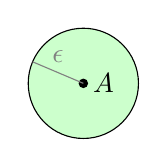
\begin{tikzpicture}
\filldraw[fill=green!20] (0,0) circle (7mm);
\filldraw[black] (0,0) circle (1.5pt) node[anchor=west] {$A$};
\draw[gray] (0,0) -- ++(157:7mm) node[midway,above] {$\epsilon$};
\end{tikzpicture}
\end{wrapfigure}
\[
\Pi_\epsilon(A) = \left\lbrace P \in  \mathbb R ^n : d(P,A) < \epsilon \right\rbrace
\]

\paragraph{Σημείο συσσώρευσης} \hspace{0pt} \\


\begin{wrapfigure}{l}{0.3\textwidth}
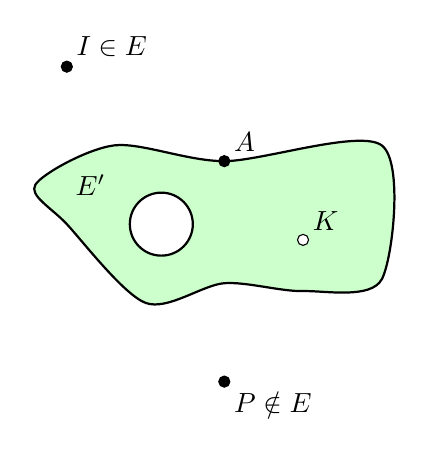
\begin{tikzpicture}
\filldraw[thick,fill=green!20] plot [smooth cycle] coordinates {
(0,0) (-0.4, 0.5) (0.6, 1) (2,0.8) ( 4,1) (4,-0.7) (3,-0.85) (2, -0.75) (1,-1)
};
\filldraw[thick,fill=white] (1.2,0) circle (4mm);
\filldraw[fill=white] (3,-0.2) circle(2pt) node[anchor=south west] {$K$};
\draw (0.3,0.5) node {$E'$};
\filldraw (2,0.8) circle(2pt) node[anchor=south west] {$A$};

\filldraw (0,2) circle(2pt) node[anchor=south west] {$I \in E$};
\filldraw (2,-2) circle(2pt) node[anchor=north west] {$P \notin E$};
\end{tikzpicture}
\vspace{-40pt}
\end{wrapfigure}

\( E = (E' - \lbrace K\rbrace ) \cup \lbrace I\rbrace \)



\begin{itemize}
\item Σημείο συσσώρευσης: \( \left( \Pi_\epsilon(P) - \left\lbrace P \right\rbrace \right) \cap E \neq \emptyset \)
\item Παράγωγο σύνολο: \(Ε'\) (τα σημεία συσσώρευσης του \(Ε\))
\item Κλειστότητα του \(Ε\): \(Ε \cup E'\)
\item Συνοριακό σημείο \(Α\): \(\forall \epsilon > 0: \Pi_\epsilon(A) \cap E \neq \emptyset\) και \(\Pi_\epsilon(A) \cap \left( \mathbb R^n - E \right) \neq \emptyset\) (το \(Ε\) αλλά και το συμπληρωματικό του ανήκουν σε κάθε περιοχή του \(Α\)).
\item Κλειστό σύνολο: Συμπεριλαμβάνει το σύνορο
\item Ανοικτό σύνολο: Δεν συμπεριλαμβάνει κανένα συνοριακό σημείο
\item Οι χώροι \(\emptyset\) και \( \mathbb R ^ n \) θεωρούνται κλειστοί και ανοικτοί.
\end{itemize}

\paragraph{Συνεκτικό σύνολο (ή συναφές)}
Κάθε δύο σημεία του συνόλου μπορούν να ενωθούν με μια γραμμή που ανήκει στο σύνολο.

\paragraph{Κυρτό σύνολο}
Κάθε δύο σημεία του συνόλου μπορούν να ενωθούν με \textit{ευθεία} γραμμή που ανήκει στο σύνολο.

\paragraph{Απλά συνεκτικό σύνολο}
Κάθε καμπύλη του συνόλου θα ανήκει μέσα στο σύνολο αν τη σφίξω.

\paragraph{} \hspace{0pt} \\
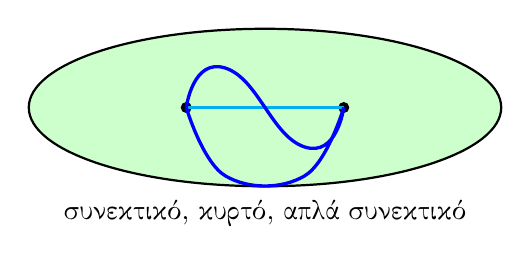
\begin{tikzpicture}
\filldraw[thick,fill=green!20] plot [smooth cycle,tension=1] coordinates {
(0,0) (3,1) (6,0) (3,-1)
};
\fill (2,0) circle (2pt);
\fill (4,0) circle (2pt);
\draw[very thick,cyan] (2,0)--(4,0);
\draw[very thick,blue] plot[smooth,tension=1] coordinates {(2,0) (2.5,0.5)  (3.5,-0.5) (4,0)};
\draw[very thick,blue] plot[smooth,tension=0.7] coordinates {(2,0) (2.5,-0.87)  (3.5,-0.87) (4,0)};
\node[anchor=north] at (current bounding box.south) {συνεκτικό, κυρτό, απλά συνεκτικό};
\end{tikzpicture}
\hspace{10pt}
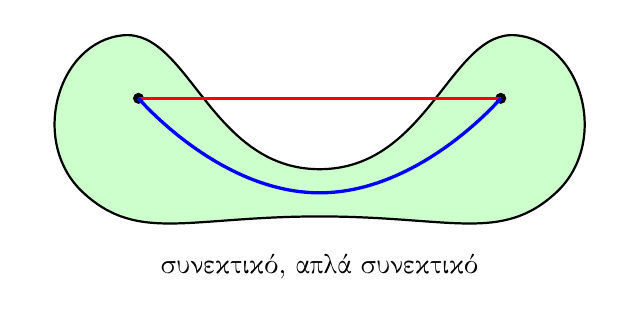
\begin{tikzpicture}
\filldraw[thick,fill=green!20] plot [smooth cycle,tension=1] coordinates {
(0,0) (0.5,2) (3,0.3) (5.5,2) (6,0) (3,-0.3)
};
\fill (0.7,1.2) circle (2pt);
\fill (5.3,1.2) circle (2pt);
\draw[very thick,red] (0.7,1.2)--(5.3,1.2);
\draw[very thick,blue] plot[smooth,tension=1] coordinates {(0.7,1.2) (3,0) (5.3,1.2)};
\node[anchor=north] at (current bounding box.south) {συνεκτικό, απλά συνεκτικό};
\end{tikzpicture}

\paragraph{} \hspace{0pt} \\
%\\
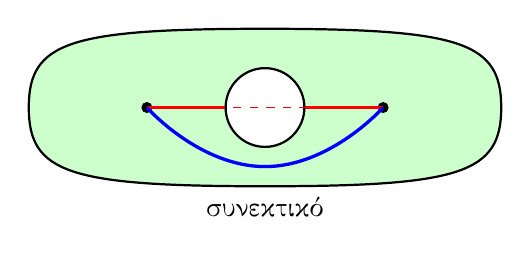
\begin{tikzpicture}
%\filldraw[thick,fill=green!20] (0,0) ellipse (3 and 2);
\filldraw[thick,fill=green!20] plot [smooth cycle,tension=1.5] coordinates {
(0,0) (3,1) (6,0) (3,-1)
};
\fill (1.5,0) circle (2pt);
\fill (4.5,0) circle (2pt);
\draw[very thick,red] (1.5,0)--(4.5,0);
\filldraw[thick,fill=white!20] (3,0) circle (0.5);
\draw[dashed,red] (1.75,0)--(4.25,0);
\draw[very thick,blue] plot[smooth,tension=1] coordinates {(1.5,0) (3,-0.75) (4.5,0)};
\node[anchor=north] at (current bounding box.south) {συνεκτικό};
\end{tikzpicture}
\hspace{40pt}
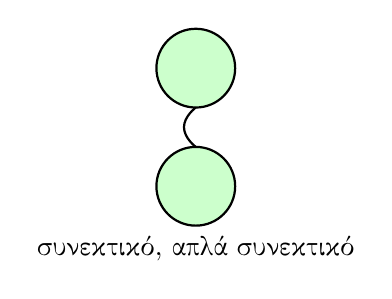
\begin{tikzpicture}
\filldraw[thick,fill=green!20] (0,0.75) circle (0.5);
\filldraw[thick,fill=green!20] (0,-0.75) circle (0.5);
\draw[thick] plot[smooth,tension=1] coordinates {(0,0.25) (-0.15,0) (0,-0.25)};
\node[anchor=north] at (current bounding box.south) {συνεκτικό, απλά συνεκτικό};
\end{tikzpicture}
\hspace{40pt}
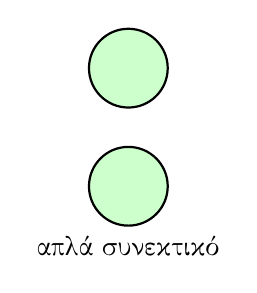
\begin{tikzpicture}
\filldraw[thick,fill=green!20] (0,0.75) circle (0.5);
\filldraw[thick,fill=green!20] (0,-0.75) circle (0.5);
\node[anchor=north] at (current bounding box.south) {απλά συνεκτικό};
\end{tikzpicture}

\paragraph{}
Η μόνη συσχέτιση που ισχύει είναι η εξής:
\begin{align*}
\text{κυρτό} &\implies \text{συνεκτικό} \\
\text{κυρτό} &\implies \text{απλά συνεκτικό}
\end{align*}

\begin{wrapfigure}{r}{0.3\textwidth}
\caption{Φραγμένο σύνολο}
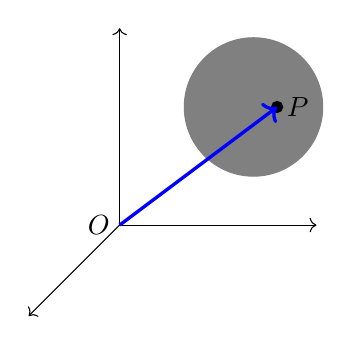
\begin{tikzpicture}
\draw[->] (xyz cs:x=0) -- (xyz cs:x=2.5);
\draw[->] (xyz cs:y=0,x=0) -- (xyz cs:y=2.5,x=0);
\draw[->] (xyz cs:z=0,x=0) -- (xyz cs:z=3,x=0);

\node (0,0) [anchor=east] {\(O\)};

\filldraw[gray] (1.7,1.5) circle (25pt) node[anchor=north] {\(E\)};

\filldraw[black] (2,1.5) circle (2pt) node[anchor=west] {\(P\)};
\draw[->,blue, very thick,anchor=west] (0,0) -- (2,1.5);
\end{tikzpicture}
\end{wrapfigure}

\paragraph{Φραγμένο σύνολο} ανν \(\norm{\overrightarrow{OP}} = d(O,P)\) πεπερασμένη
\paragraph{Συμπαγές σύνολο} ανν είναι φραγμένο και περιέχει το σύνορο

\subsubsection{Ορισμός συνάρτησης}

\(E \subseteq   \mathbb R^n, \quad B \subseteq  \mathbb R \)
\[f: E \rightarrow B: z = f(x_1, \dots, x_n) \]
\[P = \left( x_1, \dots, x_n \right) \rightarrow \text{πρότυπα ή αρχέτυπα, }z\text{ εικόνες} \]


\begin{wrapfigure}{r}{0.25\textwidth}
\centering
\caption{Τρισορθογώνιο σύστημα συντεταγμένων}
\begin{tikzpicture}[scale=0.7]
\draw[->] (xyz cs:x=0) -- (xyz cs:x=2.5);
\draw[->] (xyz cs:y=0,x=0) -- (xyz cs:y=2.5,x=0);
\draw[->] (xyz cs:z=0,x=0) -- (xyz cs:z=2.5,x=0);
\end{tikzpicture}
\end{wrapfigure}
Για συνάρτηση από το \( \mathbb R ^n\), χρειάζομαι \(n+1\) άξονες. Άρα γραφικές παραστάσεις θα κάνουμε για συναρτήσεις το πολύ 2 μεταβλητών, με προοπτική παράσταση ή ισουψείς καμπύλες.



\iffalse
\begin{figure}[H]
\centering
\begin{subfigure}[b]{0.44\textwidth}
\begin{tikzpicture}[scale=0.9]
\begin{axis}
[
    view={0}{90}
]
\addplot3[
    contour gnuplot={levels={0.8, 0.4, 0.2, -0.2}}
]
{sin(deg(sqrt(x^2+y^2)))/sqrt(x^2+y^2)};
\end{axis}
\end{tikzpicture}
    \end{subfigure}
\quad
\begin{subfigure}[b]{0.44\textwidth}

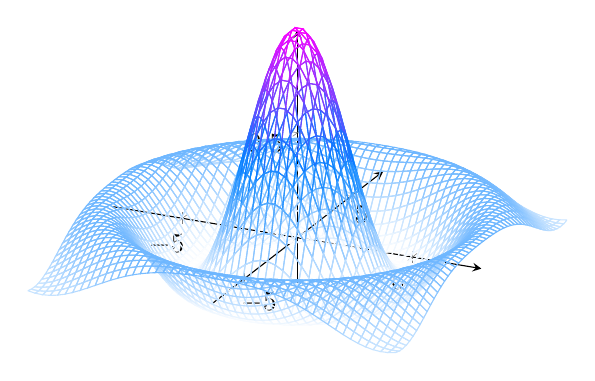
\begin{tikzpicture}
\begin{axis}[
    axis lines = middle,
    colormap/cool,
]
\addplot3[
    mesh,
    samples=50,
    domain=-8:8,
]
{sin(deg(sqrt(x^2+y^2)))/sqrt(x^2+y^2)};
\end{axis}
\end{tikzpicture}
\end{subfigure}

%\caption{Τρισδιάστατη γραφική παράσταση}
\end{figure}
\fi




\paragraph{Πολυωνυμική συνάρτηση}
Περιέχει όρους της μορφής \(a x_1^{m_1} x_2^{m_2} \cdots x_n^{m_n}, \quad m_1,m_2,\dots,m_n \in  \mathbb N \).


\textit{π.χ.}
\begin{align*}
w&=3x^4y^2z^3+4x^5yz^2-7x^3yz \\
w&=f(x,y,z)
\end{align*}
\[
\mathrm{max} \left( \sum_{i=1}^{n}m_i \right) = \text{βαθμός}(f)
\]

\subparagraph{Ρητή συνάρτηση}
\[
\frac{f(P)}{g(P)} =
\frac{f(x_1,\dots,x_n)}{g(x_1,\dots,x_n)}
\quad
f,g \text{ πολυωνυμικές}
\]

\subsubsection{Όριο συνάρτησης}
\[ \lim_{(x,y) \to (x_0,y_0)} f(x,y) = \lambda\]
\begin{attnbox}{}
\paragraph{Διπλά όρια}
\[ \lim_{x \to x_0} \left( \lim_{y \to y_0} f(x,y) \right), \quad
   \lim_{y \to y_0} \left( \lim_{x \to x_0} f(x,y) \right)
\] 
\tcblower
Δεν έχουν απαραίτητα σχέση με το κανονικό όριο (και μπορεί να έχουν διαφορετική τιμή)!
Η ύπαρξη ή/και ισότητα των ορίων δεν είναι διαγνωστική για το όριο της συνάρτησης. Αν υπάρχει το \(\lambda\) και \textbf{υπάρχουν} τα παραπάνω όρια, τότε είναι ίσα με \(\lambda\). Αν τα παραπάνω όρια \textbf{υπάρχουν} και \textbf{δεν} είναι ίσα, τότε το \(\lambda\) \textbf{δεν} υπάρχει.
\begin{center}
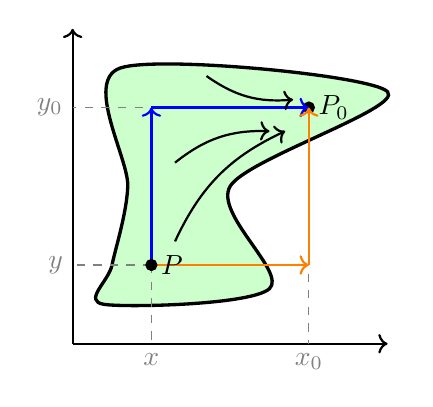
\begin{tikzpicture}
\draw[->,thick] (0,0) -- (0,4);
\draw[->,thick] (0,0) -- (4,0);

\filldraw[very thick,fill=green!20] plot [smooth cycle] coordinates {
(0.4,0.5) (0.5,1) (0.7,2) (0.6, 3.5) (4,3.2) (2,2) (2.5,0.7)
};

\draw[gray,dashed] (3,3) -- (3,0) node[anchor=north] {\(x_0\)};
\draw[gray,dashed] (3,3) -- (0,3) node[anchor=east] {\(y_0\)};
\draw[gray,dashed] (1,1) -- (1,0) node[anchor=north] {\(x\)};
\draw[gray,dashed] (1,1) -- (0,1) node[anchor=east] {\(y\)};

\filldraw[black] (3,3) circle (2pt) node[anchor=west] {\(P_0\)};

\draw[->,blue,thick] (1,1)--(1,3);
\draw[->,blue,thick] (1,3)--(3,3);

\draw[->,orange,thick] (1,1)--(3,1);
\draw[->,orange,thick] (3,1)--(3,3);

\draw[->,thick] (1.3,1.3) to [bend left=20] (2.7,2.7);
\draw[->,thick] (1.3,2.3) to [bend left=20] (2.5,2.7);
\draw[->,thick] (1.7,3.4) to [bend right=20] (2.8,3.1);


\filldraw[black] (1,1) circle (2pt) node[anchor=west] {\(P\)};
\end{tikzpicture}
\end{center}
\end{attnbox}



\begin{infobox}{Μεθοδολογία}
\begin{align*}
w&=f(x,y) \quad \text{ή}\\
w&=f(x,y,z)
\end{align*}
\[ \lim_{P\to P_0} \]
\tcblower
\begin{enumerate}
\item Επιλέγω για την \(f(x,y)\) μια καμπύλη \(y=g(x)\) του \(Ε\) που περνά από το \(Π_0\) ή \\ επιλέγω για την \(f(x,y,z)\) μια καμπύλη \(y=g(x)\) και \(z=h(x)\) του \(Ε\) που περνά από το \(Π_0\)
\item Αντικαθιστώ και καταλήγω στον υπολογισμό του ορίου \(\lim_{x \to x_0}\)
\item Αν το αποτέλεσμα εξαρτάται από τις παραμέτρους τις καμπύλης, τότε το όριο δεν υπάρχει, ενώ αν δεν εξαρτάται, το αποτέλεσμα είναι μη διαγνωστικό.
\end{enumerate}
\end{infobox}

\begin{infobox}{Μεθοδολογία}
Για όρια ρητών συναρτήσεων \(\frac{f(P)}{g(P)}\) στο \((0,0)\):
\tcblower
\begin{enumerate}
\item Αν \(B \left[ f(P) \right] > B \left[ g(P) \right]\), μάλλον το όριο υπάρχει.
\item Αν \(B \left[ f(P) \right] \leq B \left[ g(P) \right]\), μάλλον το όριο δεν υπάρχει.
\end{enumerate}
\end{infobox}

\subsubsection{Ιδιότητες ορίων}

Αν \( \lim_{P \to P_0} f(P) = \lambda_1\) και \( \lim_{P \to P_0} g(P) = \lambda_2\) τότε:

\begin{enumparen}
\item \( \lim_{P \to P_0} f(P) \pm g(P) = \lambda_1 \pm \lambda_2
\)
\item \( \lim_{P \to P_0} f(P) \cdot g(P) = \lambda_1 \cdot \lambda_2
\)
\item \( \lim_{P \to P_0} \frac{f(P)}{g(P)} = \frac{\lambda_1}{\lambda_2}
\)
\item \( \lim_{P \to P_0} \sqrt[n]{f(P)} = \sqrt[n]{\lim_{P \to P_0} f(P)} = \sqrt[n]{\lambda_1 }
\) \quad (εφ' όσον ορίζεται)
\item \( \lim_{P \to P_0} |f(P)| = |\lim_{P \to P_0} f(P)| = |\lambda_1 |
\) \quad (\(\lambda_1 >0, f(P) > 0\))
\item \( \lim_{P \to P_0} f(P)^{g(P)} = \left[ \lim_{P \to P_0} f(P) \right] ^{\lim_{P \to P_0} g(P)}
\)
\item Κρ. παρεμβολής:
\begin{enumerate}
\item \(f(P) \leq g(P) \leq h(P) \)
\item \(\lim_{P \to P_0} f(P) = \lim_{P \to P_0} h(P) = \lambda \) 
\end{enumerate}
Τότε \(\lim_{P \to P_0} g(P) = \lambda \)

\item
\begin{enumerate}
\item \( |g(P)| \leq h(P) \)
\item \(\lim_{P \to P_0} h(P) = 0 \) 
\end{enumerate}
Τότε \(\lim_{P \to P_0} g(P) = 0\)
\item
Αν \begin{enumerate*}[label={\arabic*)},font={\bfseries}]
\item \(\lim_{P \to P_0} f(P) = 0\) και
\item η \(g\) είναι φραγμένη,
\end{enumerate*}
τότε \( \lim_{P \to P_0} f(P)g(P) = 0 \).
\end{enumparen}
Προϋπόθεση για τις παραπάνω ιδιότητες είναι να μην οδηγούμαστε σε απροσδιοριστία (π.χ. \(\frac{\infty}{\infty}\))

\subsubsection{Σύνθεση συναρτήσεων}
\begin{align*}
f &: A \subseteq \mathbb R^n \to B \subseteq \mathbb R^n \\
g &: B \to C \subseteq  \mathbb R 
\end{align*}

Ορίζω:
\[
\left( g \circ f \right)(P) = g \left( f(P) \right)
\]

Έστω \( \lim _{P \to P_0} f(P) =m\). Τότε, αν οι συναρτήσεις είναι συνεχείς στο πεδίο ορισμού, έχω:
\[
\left( g \circ f \right)(P) = g(m) = \lambda
\]

\subsubsection{Συνέχεια συνάρτησης}
Μια συνάρτηση ονομάζεται συνεχής σε ένα σημείο όταν το όριό της σε εκείνο το σημείο υπάρχει και είναι ίσο με την τιμή της εκεί.

\subsubsection{}
\[\lim_{(x,y)\to(0,0)}
\]

\begin{infobox}{Μεθοδολογία}
\[ \lim_{(x,y) \to ( \pm \infty, \pm \infty )} f(x,y) \]
\tcblower
Για \(u=\frac{1}{x} \to 0, \ v=\frac{1}{y} \to 0\),
\[
\lim_{\mathclap{(x,y) \to ( \pm \infty, \pm \infty )}} f(x,y) \; = \;
\lim_{\mathclap{(u,v) \to ( 0,0 )}} f(u,v)
\]
\end{infobox}

\subsection{Ασκήσεις}
\paragraph{(1)}
\[
\lim_{(x,y) \to (2,3)} \frac{x^2+y}{x+y^3} + \cos (xy) = \frac{7}{29} + \cos(6)
\]
\paragraph{(2)}
\[
\lim_{(x,y) \to (0,0)} \frac{xy^4}{(x^2+y^2)^2}
\]

Αντικαθιστώ με πολικές συντεταγμένες:
\[
\attnboxed{\begin{cases}x = r \cos \theta \\ y = r \sin \theta\end{cases}}
\]

\begin{align*}
\lim_{(x,y) \to (0,0)} \frac{xy^4}{(x^2+y^2)^2} \\
= \lim_{r \to 0^+} \frac{r \cos \theta \, r^4 \sin^4 \theta}{r^4} \\
= \lim_{r \to 0^+} r \cos \theta \sin^4 \theta = 0
\end{align*}


\paragraph{(3)}
\[
\lim_{(x,y) \to (0,0)} \frac{x^2y}{(x^2-y^2)^2}
\]

Θέτω \(x = \lambda \sqrt y \implies y = \frac{1}{\lambda^2} x^2 \).
\begin{align*}
&\lim_{(x,y) \to (0,0)} \frac{x^2y}{(x^2-y^2)^2} \\
&= \lim_{\lambda \to 0^+} \frac{\lambda^2 |y| \cdot y}{\left( \lambda^2 |y| + y \right)^2} \\
&= \lim_{\lambda \to 0^+} \frac{\lambda^2 y^2}{\left( \lambda^2 y + y \right)^2} \\
&= \lim_{\lambda \to 0^+} \frac{\lambda^2 y^2}{y^ 2 \left( \lambda^2 +1 \right)^2} \\
&= \frac{\lambda^2}{(\lambda^2+1)^2}
\end{align*}
Άρα το όριο δεν υπάρχει.

\paragraph{(4)}
\[
\lim_{(x,y) \to (\infty,\infty)} \frac{x+2y}{x^2+y^2}
\]

\(u=\frac{1}{x} \to 0, \ v = \frac{1}{y} \to 0\)
\begin{align*}
&\lim_{(x,y) \to (\infty,\infty)} \frac{x+2y}{x^2+y^2}
\\ &=
\lim_{(u,v) \to (0,0)} \frac{\frac{1}{u} + \frac{2}{v}}{\frac{1}{u^2}+ \frac{1}{v^2}}
\\ &=
\lim_{(u,v) \to (0,0)} \frac{u^2v^2 \left( \frac{1}{u}+\frac{2}{v} \right)}{u^2v^2 \left( \frac{1}{u^2}+\frac{1}{v^2} \right)}
\\ &=
\lim_{(u,v) \to (0,0)} \frac{uv (2u+v)}{u^2+v^2}
\end{align*}

\(u =r\cos \theta,\ v=r\sin\theta\)
\begin{align*}
\lim_{r \to 0} \frac{r\cos\theta\sin\theta (2r \cos\theta + r \sin\theta)}{r^2} &= \\
\lim_{r \to 0} r\cos\theta\sin\theta (2\cos\theta+\sin\theta) = 0
\end{align*}


\paragraph{(5)}
\[
\lim_{(x,y,z) \to (0,0,0)} \frac{x^2yz}{x^2+y^2}
\]

Αντικαθιστώ με σφαιρικές συντεταγμένες:
\[
\attnboxed{\begin{cases}x = r \sin\theta\cos\phi \\ y = r \sin \theta\sin\phi \\ z = r\cos\theta \end{cases}}
\]

\begin{align*}
&\lim_{r \to 0} \frac{r^2\sin^2\theta\cos^2\phi \, r\sin\theta\sin\phi\, r \cos\theta}{r^2} \\ &=
\lim_{r \to 0} r^2(\sin^3\theta\cos\theta\cos^3\phi\sin\phi) = 0
\end{align*}


\paragraph{(6)}
\[
\lim_{(x,y,z) \to (0,0)} \frac{x+y}{x^2+y^2}
\]

\begin{align*}
\lim_{(x,y) \to (0,0)} \frac{x+y}{x^2+y^2}
\\ &=
\lim_{x \to 0} \frac{x+\lambda x}{x^2+\lambda^2 x^2}
\\ &=
\lim \frac{x(1+\lambda)}{x^2(1+\lambda^2)}
\\ &=
\lim_{x \to 0^+} \frac{1+\lambda}{x(1+\lambda^2)}
\\ &=
\frac{1+\lambda}{0^+ (1+\lambda^2)}
\end{align*}
Ανάλογα με το πρόσημο του \((1+\lambda)\), μπορεί να το όριο να είναι \(\pm\) σε πρόσημο, άρα δεν υπάρχει.

\paragraph{}
\begin{attnbox}{}
Κανόνα \textlatin{De L' Hospital} δεν μπορώ να χρησιμοποιήσω σε συναρτήσεις πολλών μεταβλητών, παρά μόνο όταν έχω μόνο μία μεταβλητή!
\end{attnbox}

\begin{align*}
\lim_{(x,y)\to(0,0)}
\frac{1-cos \sqrt{x^2+y^2}}{x^2+y^2} &= \\
&= \lim_{r\to 0^+} \frac{1-\cos r}{r^2} \\
&= \lim_{r\to 0^+} \frac{(1-\cos r)'}{(r^2)'} \\
&= \lim_{r\to 0^+} \frac{\sin r}{2r} \\
&= \lim_{r\to 0^+} \frac{(\sin r)'}{(2r)'} \\
&= \lim_{r\to 0^+} \frac{\cos r}{2} = \frac{1}{2}
\end{align*}

\paragraph{}
\begin{align*}
\lim_{(x,y)\to (0,0)}
\left[
\frac{(2+y^3)\tan (x^3+y^3)}{x^3+y^3} +
\frac{\tan(x^5y^5)}{\tan(x^5)\tan(y^5)}
\right]
&= \\
&= 
\lim_{(x,y)\to (0,0)} (2+y^3) \cdot
\lim_{(x,y)\to (0,0)} \frac{\tan(x^3+y^3)}{x^3+y^3} +
\lim_{(x,y)\to (0,0)} \frac{\tan(x^5+y^5)}{\tan(x^5) \tan(y^5)}
\end{align*}

Αν θέσω \(x^3+y^3=u\), έχω:
\[
\lim_{(x,y)\to (0,0)} \frac{\tan(x^3+y^3)}{x^3+y^3}
= \lim_{u\to 0} \frac{\tan u}{u} =
\lim_{u\to 0} \frac{(\tan u)'}{u'} =
\lim_{u \to 0} \frac{1}{\cos^2 u} = 1
\]

\[
\lim_{(x,y)\to (0,0)} \frac{\tan(x^5+y^5)}{\tan(x^5) \tan(y^5)}
=
\lim_{(x,y)\to (0,0)} \frac{\frac{\tan(x^5+y^5)}{x^5y^5}}{\frac{\tan(x^5)}{x^5}\cdot\frac{\tan(y^5)}{y^5}}
=
\frac{
\lim_{v\to 0} \frac{\tan v}{v}
}{
\lim_{w\to 0} \frac{\tan w}{w}
\cdot
\lim_{z\to 0} \frac{\tan z}{z}
}
\quad 
\left(
\begin{matrix}
x^5y^5 &=v\\
x^5 &=w\\
y^5 &=z
\end{matrix}
\right)
\]

Άρα \(\lim \bigg( \cdots \bigg) = 3\).

\paragraph{}
\[
\lim_{(x,y) \to (0,0)} y^x \quad (y \geq 0)
\]
\subparagraph{(1) \(y=0\)}
\[
\lim_{(x,y)\to(0,0)}y^x=
\lim_{x\to 0^+} 0^x = 0
\]
\subparagraph{(2) \(y=x\)}
\begin{gather*}
\lim_{(x,y)\to(0,0)}y^x=
\lim_{x\to 0^+} x^x = 0 =
\lim_{x\to 0^+} e^{\ln x^x} = \\
\lim_{x\to 0^+} e^{x\ln x} =
e^{\lim_{x\to 0^+} \ln x^x} =
e^{\lim_{x\to 0^+} \frac{\ln x}{\frac{1}{x}}} = \\
e^{\lim_{x\to 0^+} \frac{(\ln x)'}{\left(\frac{1}{x}\right) ' }} =
e^{\lim_{x\to 0^+} \left( \frac{\frac{1}{x}}{-\frac{1}{x^2}} \right)} =  
e^{\lim_{x\to 0^+} -x} = \mathbf 1
\end{gather*}

Επομένως το ζητούμενο όριο δεν υπάρχει.

\paragraph{}
\[
\lim_{(x,y) \to(0,0)} \frac{x^2y^2}{x^2y^2+(x-y)^2}
\]

Θέτοντας \(y=\lambda x\), έχω:
\begin{align*}
\lim_{(x,y) \to(0,0)} \frac{x^2y^2}{x^2y^2+(x-y)^2}
&= \\ &=
\lim_{x \to 0} \frac{\lambda^2x^4}{\lambda^2x^4+x^2(1-\lambda)^2} \\
&=
\lim_{x \to 0} \frac{\lambda^2x^2}{\lambda^2x^2+x^2(1-\lambda)^2}
\end{align*}

Για \(\lambda=1\), γίνεται \(\lim_{x\to 0} \frac{x^2}{x^2}=1\).

Για \(\lambda=-1\), γίνεται \(\lim_{x\to 0} \frac{x^2}{x^2+4} = 0\).

Παρατηρούμε ότι για δύο διαφορετικές διαδρομές έχουμε διαφορετικό αποτέλεσμα, άρα το όριο δεν υπάρχει.

\paragraph{}
\begin{align*}
\lim_{(x,y,z)\to(0,0,0)} \frac{xy^2z^3}{x^2+y^2+z^2}
&=\\&=
\lim_{r\to0^+} \frac{r\sin\theta\cos\theta \cdot r^2\sin^2\theta\sin^2\phi \cdot r^3\cos^3\theta}{r^2} \\ &=
\lim_{r\to0^+} \underbrace{r^4}_{0} \cdot \big( \underbrace{ \cdots }_\text{φ} \big) = 0
\end{align*}

\paragraph{}
\begin{align*}
\lim_{(x,y)\to(0,0)} \frac{x+y+x^2}{x-y}
&= \\ &=
\lim_{r\to0^+} \frac{r\cos\phi+r\sin\phi+r^2\cos^2\phi}{r(\cos\phi-\sin\phi)}
\\ &= \lim
\frac{\cos\phi+\sin\phi}{\cos\phi-\sin\phi} + r
\frac{\cos^2\phi}{\cos\phi-\sin\phi}
\end{align*}
Επειδή παρατηρώ ότι υπάρχει πιθανότητα απροσδιοριστίας, θα προσπαθήσω να αποδείξω ότι δεν υπάρχει το όριο.

Θέτω \(y = \lambda x\):
\begin{align*}
\lim_{x\to0}\frac{x+\lambda x+x^2}{x-\lambda x} =
\lim_{x\to0}\frac{x(1+\lambda+x)}{x(1-\lambda)} =
\lim_{x\to0}\frac{1+\lambda+x}{1-\lambda} = \frac{1+\lambda}{1-\lambda}
\end{align*}

\paragraph{}
\begin{align*}
\lim_{(x,y)\to(0,0)} |x|^{|\frac{1}{y}|} &=
\lim_{(x,y)\to(0,0)} e^{\ln|x|^{|\frac{1}{y}|}} \\ &=
\lim_{(x,y)\to(0,0)} e^{\frac{1}{y} \ln |x|} \\ &=
e^{  \lim_{(x,y)\to(0,0)} \frac{\ln|x|}{y}   } \\ &=
e^{ \frac{\lim_{x\to0} \ln|x|  }{\lim_{y\to0} |y| }} \\ &=
e^\frac{-\infty}{0^+} \\ &= e^{-\infty} = 0
\end{align*}

\paragraph{}
\begin{align*}
\lim_{(x,y)\to (0,0)} \frac{x+y-1}{\sqrt{x}-\sqrt{1-y}} &= \\ &=
\lim_{(x,y)\to (0,0)} \frac{
(x+y-1) \left(   \sqrt{x}+\sqrt{1-y}     \right)
}{
\left(
\sqrt{x}-\sqrt{1-y}
\right)
\left(
\sqrt{x}+\sqrt{1-y}
\right)
} \\ &=
\lim_{(x,y)\to (0,0)}
\frac{
(x+y-1)\left(
\sqrt{x}+\sqrt{1-y}
\right)
}{
(\sqrt{x})^2-(\sqrt{1-y})^2
} \\ &=
\lim_{(x,y)\to(0,0)}
\frac{(x+y-1)(\sqrt{x}+\sqrt{1-y}}{|x|-|1-y|} \\ &=
\lim_{(x,y)\to(0,0)}
\frac{(x+y-1)(\sqrt{x}+\sqrt{1-y})}{x-(1-y)} = 0
\end{align*}


\paragraph{}
\begin{align*}
 \lim_{(x,y)\to(0,0)} \frac{\sin x + \sin y}{\tan(2x)+\sin y}
\end{align*}

\subparagraph{(1) \(y=x\)}
\begin{align*}
\lim_{x\to0}\frac{\sin x + \sin x}{\tan(2x)+\sin x} =
\lim_{x\to0}\frac{2\sin x}{\tan (2x) + \sin x} 
 = \lim_{x\to0}
 \frac{2\cos x}{\frac{2}{\cos^2(2x)+\cos x}}
 = \frac{2}{\frac{2}{1}+1} = \frac{2}{3}
\end{align*}
\subparagraph{(2) \(y=-x\)}
\[
\lim_{x\to0}
\frac{\sin x-\sin x}{\tan(2x)-\sin x}
= \lim_{x\to0} \frac{0}{\tan(2x)-\sin x} = 0
\]

Άρα το όριο δεν υπάρχει.

\paragraph{}
\begin{align*}
 \lim_{(x,y)\to(0,0)} \frac{\sqrt{x+y}-\sqrt{x-y}}{x}
\end{align*}
Θα βρω το πεδίο ορισμού:

\[
\begin{cases}
x+y \geq 0 &\implies y \geq -x \\
x-y \geq 0 &\implies y \leq x \\
x \neq 0
\end{cases}
\]
%TODO Zaharis Graph 02

Επειδή το \((0,1)\) είναι απομονωμένο σημείο (δεν είναι σημείο συσσώρευσης), δεν έχει νόημα ο υπολογισμός του ορίου εκεί.

\paragraph{}
\begin{align*}
 &\lim_{(x,y)\to(\infty,\infty)}
 e^{\frac{x+y}{x^2+y^2}}
 \left[
 1+ \sin \left(
 \frac{3}{|x|+|y|}
 \right)
 \right]^{|x|+|y|}
 = \\ &=
\lim_{r\to\infty}
e^{\frac{r\cos\phi+r\sin\phi}{r^2}}
\left[
 1+ \sin \left(
 \frac{3}{r\left(|\cos\phi|+|\sin\phi|\right)}
 \right)
 \right]^{r\left(|\cos\phi|+|\sin\phi|\right)}
 \\ &=
\cancelto{1}{\lim_{r\to\infty} e^{ \frac{\cos\phi+\sin\phi}{r}  }}
\cdot
\lim_{r\to\infty}
\left[
 1+ \sin \left(
 \frac{3}{r\left(|\cos\phi|+|\sin\phi|\right)}
 \right)
 \right]^{r\left(|\cos\phi|+|\sin\phi|\right)}
\end{align*}

Θέτω \(t=\frac{1}{r\left(|\cos\phi|+|\sin\phi|\right)}\), άρα το όριο γίνεται:
\begin{align*}
& \lim_{t\to0^+}
\left[
1+\sin(3t)
\right]^\frac{1}{t} \\
&=
e^{\lim_{t\to0^+} \ln \left[
1+\sin(3t)
 \right]^\frac{1}{t}}
 \\ &=
e^{\lim_{t\to0^+} \frac{\ln \left[
1+\sin(3t)\right]}{t}
 } \\
 &=
 e^{
 \lim{t\to0^+}
 \frac{3\cdot\cos(3t)}{1+\sin(3t)}
 }
\end{align*}

\paragraph{}
\begin{align*}
 \lim_{(x,y,z)\to(0,0,0)} \frac{x^2-y^2+2y^3-z}{x^2+y^2+z^2}
\end{align*}
Θέτω \(\begin{cases}y=\lambda x\\ z = \mu x\end{cases}\). Το όριο γίνεται:
\begin{align*}
& \lim_{x\to0^+}
\frac{x^2-\lambda^2x^2+2\lambda^3x^3-\mu x}{x^2+\lambda^2+\mu ^2 x^2}
\\ &=
\lim_{x\to0^+}
\frac{x(x-\lambda^2x+2\lambda^3x^2-\mu)}{x^2(1+\lambda^2+\mu^2)} \\ &=
\lim_{x\to0^+}
\frac{x(1-\lambda^2)+2\lambda^3x^2-\mu}{x(1+\lambda^2+\mu^2)} = \frac{-\mu}{0} =
\begin{cases}
-\infty &= \text{ για } \mu = 1 \\
\infty &= \text{ για } \mu = -1
\end{cases}
\end{align*}



\paragraph{}
\[
f(x,y) = \frac{xy}{x^2+y^2}+x^2y \sin \left(\frac{1}{x^2} \right)
\]
Όριο, διπλά όρια?

\begin{gather*}
 \lim_{(x,y)\to (0,0)} f(x,y) = 
  \lim_{(x,y)\to (0,0)} 
	\left[
\frac{xy}{x^2+y^2}
+ x^2y\sin \left( \frac{1}{x^2} \right)
	\right]
	=
	 \lim_{(x,y)\to (0,0)}  \frac{xy}{x^2+y^2}
+ \lim_{(x,y)\to (0,0)} 
\underbrace{x^2y}_\text{μ} \underbrace{\sin \left( \frac{1}{x^2} \right)}_\text{φ}
\\
 \lim_{r\to0^+} \frac{r\cos\theta \ r\sin\theta}{r^2}
 = \lim_{r\to0^+} \cos\theta \ \sin\theta
\end{gather*}
Εναλλακτικός τρόπος:
\[y=\lambda x,\quad  \lim_{x\to0}  \frac{\lambda x^2}{x^2(1+\lambda^2)} = \frac{\lambda}{1+\lambda^2}\]
Άρα δεν υπάρχει το όριο.

Για τα διπλά όρια:
\[
\lim_{y\to0}
\left(
\lim_{x\to0} f(x,y)
\right)
=
\lim_{y\to0} \left( \frac{0\cdot y}{0^2+y^2}+0^2y \sin \left( \frac{1}{0^2} \right) \right) = 0 = \lim_{y\to0}(0)=0
\]

\[
\lim_{x\to0}
\left(
\lim_{y\to0} f(x,y)
\right)
=
\lim_{y\to0} \left( \frac{x\cdot 0}{x^2+0^2}+x^2\cdot 0 \sin \left( \frac{x}{0^2} \right) \right) = 0 = \lim_{x\to0}(0)=0
\]
Παρατηρούμε ότι τα διπλά όρια υπάρχουν και είναι ίσα μεταξύ τους, αλλά το όριο της συνάρτησης δεν υπάρχει.

\paragraph{Άσκηση}
\[ f(x,y,z) = \frac{x\sin x + y\sin y + z\sin z}{x^2+y^2+z^2} 
\quad \mathbb R^3 -  \left\lbrace (0,0,0) \right\rbrace
\]
Τροποποίηση συνάρτησης ώστε να είναι συνεχής σε όλο το \(\mathbb R^3\), δηλαδή:
\[
f(x,y,z) = \begin{cases}
\frac{\cdots}{\cdots}, \quad &  \mathbb R ^3 -  \left\lbrace (0,0,0) \right\rbrace \\
??? & (0,0,0)
\end{cases}
\]

\begin{align*}
 & \lim_{\mathclap{(x,y,z)\to (0,0,0)} }
 \frac{x\sin x + y\sin y + z\sin z}{x^2+y^2+z^2} 
 =
  \lim_{(x,y,z)\to (0,0,0)} 
\left(
\frac{x^2}{x^2+y^2+z^2} \frac{\sin x}{x}
+\frac{y^2}{x^2+y^2+z^2} \frac{\sin y}{y}
+\frac{z^2}{x^2+y^2+z^2} \frac{\sin z}{z}
\right)
\\ &=
 \lim_{(x,y,z)\to (0,0,0)} \frac{x^2}{x^2+y^2+z^2}
\cdot \cancelto{1}{\lim_{x\to0} \frac{\sin x}{x}}
 + \lim_{(x,y,z)\to 0} \frac{y^2}{x^2+y^2+z^2}
\cdot \cancelto{1}{\lim_{y\to0} \frac{\sin y}{y}}
 + \lim_{(x,y,z)\to 0} \frac{z^2}{x^2+y^2+z^2}
\cdot \cancelto{1}{\lim_{z\to0} \frac{\sin z}{z}}
\\ &=
 \lim_{(x,y,z)\to (0,0,0)} 
 \frac{x^2+y^2+z^2}{x^2+y^2+z^2} =1 
\end{align*}

Άρα τελικά:
\[
f(x,y,z) = \begin{cases}
\frac{\cdots}{\cdots}, \quad &  \mathbb R ^3 -  \left\lbrace (0,0,0) \right\rbrace \\
1 & (0,0,0)
\end{cases}
\]

\paragraph{Άσκηση}
\[
f(x,y) = \frac{\sin x - \sin y}{\tan x - \tan y},
\quad D = \overbrace{\left[
0, \frac{\pi}{4}
\right]^2}^{\left[
0, \frac{\pi}{4}
\right] \times \left[
0, \frac{\pi}{4}
\right]} - \left\lbrace (x,y):\ x=y \right\rbrace
\]

Τροποποίηση της \(f(x,y)\) ώστε η \(f(x,y)\) να είναι συνεχής στο \(\left[
0, \frac{\pi}{4}
\right]^2\)

\begin{gather*}
\frac{\sin x - \sin y}{\frac{\sin x}{\cos x}-\frac{\sin y}{\cos y}}
= \frac{\sin x - \sin y}{\frac{\sin x \cos y - \sin y \cos x}{\cos x \cos y}}
= \frac{\sin x - \sin y}{\sin (x-y)} \cos x \cos y =\\
= \frac{\cancel{2 \sin \frac{x-y}{2}} \cos \frac{x+y}{2}}{\cancel{2\sin\frac{x-y}{2}} \cos\frac{x-y}{2}}
\cos x \cos y
= \frac{\cos\frac{x+y}{2}}{\cos\frac{x-y}{2}}\cos x \cos y
\end{gather*}

\begin{gather*}
 \lim_{(x,y)\to (x,x)}  f(x,y)
 = 
 \frac{\cos\frac{2x}{2}}{\cos 0} \cos x \cos x = \cos^3x
\end{gather*}

Άρα τελικά:
\[
f(x,y) = \begin{cases}
\frac{\sin x - \sin y}{\tan x - \tan y},\quad & \left[
0, \frac{\pi}{4}
\right]^2 - \left\lbrace (x,y):\ x=y \right\rbrace \\
\cos^3x,\quad & x=y
\end{cases}
\]

\subsection{Κατευθυνόμενη Παράγωγος}
%TODO Zaharis Graph 01
%TODO Zaharis Graph 02
\[
\pd{F(P_0)}{\vec{a}} = \nabla_{\vec{a}} f(P_0) = \vec{D}_{\vec{a}} f(P_0)
= \lim_{t\to0} \frac{\overbrace{f(P_0 +t\vec{a})}^{f(P)} - f(P_0)}{t}
= \lim_{t\to0} \frac{f(\vec{r}_{P_0}+t\vec{a})-f(\vec{r_{P_0}})}{t}
\]

\[
\frac{\Delta f}{t} = \tan \phi
\]

Μερικές παράγωγοι:
\begin{align*}
\frac{\partial f(P_0)}{\partial \vec{e_1}} &= \frac{\partial f(P_0)}{\partial x} = \lim_{t\to0} \frac{f(x_0+t,y_0)-f(x_0,y_0)}{t} \\
\frac{\partial f(P_0)}{\partial \vec{e_2}} &= \frac{\partial f(P_0)}{\partial y} = \lim_{t\to0} \frac{f(x_0,y_0+t)-f(x_0,y_0)}{t} \\
\end{align*}
(αντίστοιχα ορίζονται και για περισσότερες διαστάσεις - δε συμπεριλαμβάνεται σε αυτόν τον ορισμό ο άξονας των \(z\), αφού δεν είναι μέρος του πεδίου ορισμού)

\paragraph{Παράδειγμα}
Έστω \(f(x,y)=\frac{xy}{x^2+y^2}+x^2y\sin\left(\frac{1}{x^2}\right)\).

Τότε:
\begin{align*}
\pd{P(x,y)}{x} &= \frac{y(x^2+y^2)-xy\cdot2x}{(x^2+y^2)^2}
+ y \left[
2x\sin\left(\frac{1}{x^2}\right)
+x^2 \cdot \cos\left( \frac{1}{x^2}\right)\left( -\frac{2}{x^3} \right)
\right] \\
\pd{P(x,y)}{y} &=\frac{x(x^2+y^2)-xy\cdot2y}{(x^2+y^2)^2}+x^2\sin \left( \frac{1}{x^2}\right)
\end{align*}

\paragraph{}
Για να είναι συνεχής μια συνάρτηση στο σημείο \(P_0\), αρκεί:
\[
\begin{cases}
\exists f_x, f_y\quad \pi_\epsilon (P_0) \\
f_x,f_y\text{ πεπερασμένες}
\end{cases}
\implies\text{ΜΕΡΙΚΩΣ ΠΑΡΑΓΩΓΙΣΙΜΗ}
\]
Αν η συνάρτηση είναι μερικώς παραγωγίσιμη, υπάρχει η λύση (\textlatin{Gradient}) συνάρτησης.

\subsubsection{\textlatin{Gradient} συνάρτησης \(f(x_1,\dots,x_n)\)}
\begin{gather*}
\mathrm{grad}\,f = \nabla f(x_1,\dots,x_n) =
\left[
f_{x_1}(P)\dots f_{x_n}(P)
\right] \\
\nabla f = \left[ f_x f_y \right]
\end{gather*}

\subsubsection{}
\[
\nabla f(P_0) =
\left(
f_{x_1}(P_0),f_{x_2}(P_0),\dots,f_{x_n}(P_0)
\right)
\]

Η ύπαρξη του \(\nabla f(P_0)\) προϋποθέτει:
\begin{enumerate}
\item \(\exists f_{x_i}(P_0)\quad i=1,\dots,n\)
\item \(f_{x_i}(P_0) \rightarrow \text{ πεπερασμένη}\)
\end{enumerate}

\paragraph{Πότε η \(f\) είναι συνεχής στο \(P_0\)?}
%TODO Zaharis Graph 01

\paragraph{Πότε η \(f\) είναι παραγωγίσιμη (διαφορίσιμη) στο \(P_0\)?}
\begin{itemize}
\item \(\exists \ f_{x_i}\)
\item \(f_{x_i}\) συνεχείς
\end{itemize}

\subsection{}
\[
f'(x_0) = \lim_{x\to x_0}\frac{f(x)-f(x_0)}{x-x_0}
\implies
\lim_{x\to x_0} \left|
\frac{f(x)-f(x_0)-f'(x_0)(x-x_0)}{x-x_0}
\right| = 0
\]

%TODO Zaharis Graph 02
\[
\lim_{P\to P_0}
\frac{
\Big|
f(P)-f(P_0)-f'(P_0)(\overbrace{P-P_0}^{\vec{r_P}-\vec{r_{P_0}}})
\Big|
}{|\overrightarrow{PP_0}|}
\]

Τα διανύσματα γνωρίζουμε ότι γράφονται ως πίνακες μίας διάστασης:
\[
\vec{r_P}-\vec{r_{P_0}} =
\begin{bmatrix}
x_{1P}-x_{1P_0}\\
x_{2P}-x_{2P_0}\\
\vdots\\
x_{nP}-x_{nP_0}
\end{bmatrix}
\]

\[
f'(x_0)=\begin{bmatrix}
b_1&b_2&\cdots&b_n
\end{bmatrix}
\]

\begin{align*}
\lim_{t\to0}
\frac{
\left|
f(P_0+t\vec{a})-f(P_0)-f'(P_0)t\vec{a}
\right|
}{|t||\vec{a}|} = 0 &\implies \\
\lim_{t\to0}
\left|
\frac{f(P_0+t\vec{a})-f(P_0)-f'(P_0)t\vec{a}}{t}
\right| = 0 &\implies \\
\left|
\lim_{t\to0}
\frac{f(P_0+t\vec{a})}{t}
- f'(P_0)\vec{a}
\right| = 0 &\implies \\
\frac{\partial f(P_0)}{\partial \vec{a}} - f'(P_0)\vec{a} = 0 &\implies\\
\frac{\partial f(P_0)}{\partial \vec{a}} = f'(P_0)\cdot \vec{a}
\end{align*}

\paragraph{Συσχέτιση με \textlatin{Gradient}}
\begin{align*}
\pd{f(P_0)}{\vec{e_i}} = f'(P_0)\vec{e_1} &\implies \\
\pd{f(P_0)}{\vec{e_i}} = 
\begin{bmatrix}
b_1&\cdots&b_i&\cdots&b_n
\end{bmatrix}
\begin{bmatrix}
0\\ \vdots\\ 1  \\ \vdots \\ 0
\end{bmatrix} \rightarrow \text{ 1 μόνο γραμμή}
 &\implies \\
\boxed{\pd{f(P_0)}{x_1}=b_i}
\end{align*}

\[
f'(P_0) = \begin{bmatrix}
b_1&b_2&\cdots&b_n
\end{bmatrix}
=
\begin{bmatrix}
f_{x_1}(P_0)
&f_{x_2}(P_0)
&\cdots
&f_{x_n}(P_0)
\end{bmatrix}
= \mathbf{\nabla f(P_0)}
\]

Βέβαια η \(f'(P_0)\) ορίζεται μόνο αν οι επιμέρους παράγωγοι είναι συνεχείς!

\paragraph{Φυσική σημασία}
\begin{align*}
\left|
\pd{f(P_0)}{\vec{a}} 
\right|
= \left|
f'(P_0)\vec{a}
\right|
\implies
\left|
\pd{f(P_0)}{\vec{a}} 
\right|
= \left|
\nabla f(P_0)\cdot\vec{a}
\right|
\leq
\left|
\nabla f(P_0)
\right|
\cdot
\cancelto{1}{|\vec{a}|}
\implies \boxed{
\left|
\pd{f(P_0)}{\vec{a}}
\right|
\leq
\left|
\nabla f(P_0)
\right|}
\end{align*}

Άρα το \textlatin{gradient} προσδιορίζει το μέγιστο ρυθμό μεταβολής της συνάρτησης.

Το διάνυσμα της κατεύθυνσης όπου μεγιστοποιείται ο ρυθμός μεταβολής είναι το:
\[
\vec{a} = \frac{\nabla f(P_0)}{\left| \nabla f(P_0) \right|}
\]

\subsection{Θεώρημα Μέσης Τιμής}
\[
f:\underbrace{E}_{\mathclap{\text{κυρτό σύνολο}}} \subseteq  \mathbb R ^n \to R
\]

%TODO Zaharis Graph 03
Επάνω στην ευθεία που ενώνει τα \(P_0\) και \(P_1\), υπάρχει σημείο \(P^*\) τέτοιο ώστε:
\[
f(P_1)-f(P_0) = f'(P^*)\big( P_1-P_0\big)
\]

\subsubsection{Μερικές παράγωγοι ανώτερης τάξης}
\[
\frac{\partial^m f(P)}{\partial x_{km} \dots \partial x_{k2} \partial x_{k1}}
= f_{x_{k1}x_{k2}\dots x_{km}}(P) =
\frac{\partial}{\partial x_{km}}
\left(
\cdots
\left(
\frac{\partial}{\partial x_{k2}}
\left(
\frac{\partial f(P)}{\partial x_{k1}}
\right)
\right)
\right)
\]

\paragraph{π.χ.}
\[
f=f(x,y,z)
\]
\begin{gather*}
\pd{f}{x},\pd{f}{y},\pd{f}{z}\\
\frac{\partial^2 f}{\partial x \partial y},\
\frac{\partial^2 f}{\partial y \partial x},\
\frac{\partial^2 f}{\partial x \partial x},\
\frac{\partial^2 f}{\partial x \partial z},\
\frac{\partial^2 f}{\partial z \partial x},\
\frac{\partial^2 f}{\partial x \partial x}=\pd[2]{f}{x},\
\frac{\partial^2 f}{\partial y \partial y}=\pd[2]{f}{y},\
\end{gather*}

Η συνέχεια των μερικών παραγώγων μέχρι κάποια τάξη, επιτρέπει την αντιμετάθεση των παραγώγων.

Για παράδειγμα, αν η \(f\) έχει συνεχείς μερικές παραγώγους μέχρι και 2ης τάξης, ισχύει:
\begin{gather*}
\frac{\partial^2f}{\partial x\partial y} =
\frac{\partial^2f}{\partial y\partial x}\\
\frac{\partial^3f}{\partial x\partial y\partial z} \neq
\frac{\partial^3f}{\partial y\partial z\partial x}
\end{gather*}

Επίσης συμβολίζω:
\begin{gather*}
\frac{\partial f}{\partial x} = f_x\\
\frac{\partial^3 f(P)}{\partial x \partial y \partial z} = f_{zyx}(P)\\
\frac{\partial^3 f(P)}{\partial x^2 \partial y} = f_{yx^2}(P)
\end{gather*}
(προσοχή στην αλλαγή φοράς των \(x,\ y,\ z\)!)

Να σημειωθεί ότι η χρήση των \(\partial\) και \(f_{\dots}\) είναι καθαρά θέμα συμβολισμού.

\paragraph{Αρμονική συνάρτηση}
\(
f=f(_1,\dots,x_n)
\)

\[
f_{x_1^2}(P)+f_{x_2^2}(P)+\dots+f_{x_n^2}(P) = 0
\iff
\pd[2]{f(P)}{x_1}+\pd[2]{f(P)}{x_2}+\dots+\pd[2]{f(P)}{x_n}= 0
\]
και τα μέγιστα \& ελάχιστα της συνάρτησης λαμβάνονται πάνω στο όριο του πεδίου ορισμού της.

Ονομάζω το \(
\pd[2]{}{x_1}+\pd[2]{}{x_2}+\dots+\pd[2]{}{x_n}
\) τελεστή \textlatin{Laplace} (Λαπλασιανή), και συμβολίζω:

\[
\nabla^2 = \pd[2]{}{x_1}+\pd[2]{}{x_2}+\dots+\pd[2]{}{x_n} \rightarrow
\text{ Τελεστής \textlatin{Laplace}}
\]

Άρα ο επάνω ορισμός γίνεται:
\[
\iff \boxed{\nabla^2 f(P)} = 0
\]

\paragraph{Διαφορικό}
%TODO Zaharis Graph 04
\begin{align*}
\overbrace{\dif f(P_0)}^{\mathclap{\text{διαφορικό 1\textsuperscript{ης} τάξης ή ολικό διαφορικό}}} &= \pd{f(P_0)}{x}\dif x + \pd{f(P_0)}{y} \dif y
\quad (+\dots) \\
&=
\begin{bmatrix}
f_x(P_0)&f_y(P_0)
\end{bmatrix}
\begin{bmatrix}
\dif x\\ \dif y
\end{bmatrix}
= \nabla f(P_0) \dif P
= \nabla f(P_0) \dif \vec{r}
\end{align*}

\subparagraph{Διαφορικό 2\textsuperscript{ης} τάξης}
\begin{align*}
\dif^2 f  = \dif (\dif f) &= \dif
\left(
f_x \dif x + f_y \dif y
\right) \\
&= \pd{}{x} (f_x \dif x + f_y \dif y) \dif x
+ \pd{}{y} (f_x \dif x + f_y \dif y) \dif y
\\ &=
\left(
f_{x^2} \dif x + f_x \pd{\dif x}{x} + f_{yx} \dif y + f_y \cancel{\pd{\dif y}{x}}
\right) \dif x
+
\left(
f_{xy} \dif x + f_x \cancel{\pd{\dif x}{y}} + f_{y^2} \dif y + f_y \pd{\dif y}{y}
\right) \dif y
\\ &=
\underbrace{f_{x^2} (\dif x)^2}
+ f_x \dif^2 x
+ \underbrace{f_{yx} \dif y \dif x
+ f_{xy} \dif x \dif y}
+ \underbrace{f_{y^2} (\dif y)^2}
+ f_y \dif^2 y
%TODO
\\ & \overset{\mathclap{\text{εφόσον υπάρει συνέχεια παραγώγων}}}{=}
f_{x^2}(\dif x)^2
+2f_{xy} \dif x \dif y +
f_{y^2} (\dif y)^2
+ f_x \dif^2 x + f_y \dif^2 y
\end{align*}

Αν \(\dif x = \) σταθ. και \(\dif y = \) σταθ. τότε \(\dif^2 x =\dif^2 y = 0\).

\[
\dif^2 f = (f_x\dif x+f_y\dif y)^{(2)}
\]

Ομοίως
\[
\dif^3 f = (f_x\dif x+f_y\dif y)^{(3)} = f_{x^3} (\dif x)^3+3f_{x^2y}(\dif x)^2\dif y + 3 f_{xy} = \dif x (\dif y)^2 + f_{y^3} (\dif y)^3
\]

\subsubsection{Κριτήριο ύπαρξης ολικού διαφορικού}
\[
P(x,y) \dif x + Q(x,y) \dif y \qquad P,Q\to\text{συνεχείς μερικές παραγώγους 1\textsuperscript{ης} τάξης}
\]

\begin{align*}
f=f(x,y)\qquad \dif f &= P(x,y)\dif x + Q(x,y)\dif y & f_x(x,y) = P(x,y) \implies^{\pd{}{y}} f_{xy}=P_y
\\ \dif f &= f_x(x,y)\dif x + f_y(x,y)\dif y		 & f_y(x,y) = Q(x,y) \implies^{\pd{}{x}} f_{yx} = Q_x
\\
\implies \boxed{P_y=Q_x}
\end{align*}

\begin{align*}
\int_{A_0}^A \dif f=
\int_{(x_0,y_0)}^{(x,y)} \left[ P(x,y)\dif x + Q(x,y)\dif y \right]
\implies \\
f(A)-f(A_0) = 
\int_{(x_0,y_0)}^{(x,y_0)}\left[
P(x,y)\dif x +\cancel{Q(x,y)\dif y}
\right] + \int_{(x,y_0)}^{(x,y)}\left[
\cancel{P(x,y)\dif x} +Q(x,y)\dif y
\right]\implies \\ \boxed{\qquad \qquad
f(A)=f(A_0) + \underbrace{\int_{x_0}^x P(t,y_0) \dif t + \int_{y_0}^y Q(x,t)\dif t}_{\mathclap{\attnboxed{\text{προσοχή στα ορίσματα! γίνονται συχνά λάθη!}}}}
\qquad \qquad
}
\end{align*}

\paragraph{}
\(\vec F = (P,Q)\)
\[
\underbrace{df}_{\mathclap{\text{βαθμωτό ή αριθμητικό δυναμικό του πεδίου $\vec F$}}}
= \vec F \dif \vec r = (P,Q)\cdot (\dif x,\dif y) = P\dif x + Q\dif y
\]

\paragraph{Σε 3 διαστάσεις}
\[
P(x,y,z)\dif x + Q(x,y,z) \dif y + R(x,y,z)\dif z
\]
\(
f=f(x,y,z)
\)

\[
\begin{cases}
\dif f &= P(x,y,z)\dif x + Q(x,y,z)\dif y + R(x,y,z)\dif z\\
\dif f &= f_x(x,y,z)\dif x + f_y(x,y,z)\dif y + f_z(x,y,z)\dif z
\end{cases}
\implies
\begin{cases}
f_x&=P\\
f_y&=Q\\
f_z&=R
\end{cases}
\implies
\begin{cases}
\begin{cases}
f_{xy}&=P_y\\
f_{yx}&=Q_x
\end{cases}
&\implies P_y=Q_x\\
\begin{cases}
f_{yz}&=Q_z\\
f_{zy}&=R_y
\end{cases}
&\implies Q_z=R_y\\
\begin{cases}
f_{xz}&=P_z\\
f_{zx}&=R_x
\end{cases}
&\implies P_z=R_x
\end{cases}
\]

\begin{align*}
\begin{cases}
\dif f& = P\dif x  + Q\dif y + R\dif z = (P,Q,R)\cdot (\dif x,\dif y,\dif z)  = \vec F\cdot \dif \vec r \\
\dif f &= f_x\dif x +f_y\dif y +f_z\dif z = (f_x,f_y,f_z)(\dif x,\dif y,\dif z) = \nabla f \dif \vec r
\end{cases}
&\implies
\vec F = \nabla f \\&
\implies \nabla \times \vec F = \nabla \times \nabla f \\ &\implies \boxed{
\nabla \times \vec F = 0
}
\end{align*}

\(\vec F = (P,Q,R)\)
\begin{align*}
\nabla \times \vec F &= \left|
\begin{matrix}
\overrightarrow{e_1}&\overrightarrow{e_2}&\overrightarrow{e_3}\\
\pd{}{x}&\pd{}{y}&\pd{}{z}\\
P&Q&R
\end{matrix}
\right|
=
\overrightarrow{e_1}\left(
\pd{R}{y}-\pd{Q}{z}
\right)
-
\overrightarrow{e_2}\left(
\pd{R}{x}-\pd{P}{z}
\right)
+
\overrightarrow{e_3}\left(
\pd{Q}{x}-\pd{P}{y}
\right)\\
\nabla \times \vec F &= \vec e_1 (R_y-Q_z) - \vec e_2 (R_x-P_z) + \vec e_3 (Q_x-P_y) = 0 \implies
\begin{cases}
R_y&=Q_z\\
R_x&=P_z\\
Q_z&=P_y
\end{cases}
\end{align*}

\subparagraph{Αστρόβιλο πεδίο}
\begin{enumparen}
\item \(\vec F = \nabla f\)
\item \(\nabla \times \vec F = 0\)
\item \( \int_{A_0}^A \vec F\dif\vec r = f(A)-f(A_0)\)
\end{enumparen}

\[
\int_{A_0}^A \vec F \dif r = \int_{A_0}^A \nabla f \dif \vec r = \int_{A_0}^A \dif f = f(A)-f(A_0)
\]

Ένα αστρόβιλο πεδίο είναι και συντηρητικό όταν ο χώρος είναι απλά συνεκτικός.

\paragraph{}
%TODO Zaharis Graph 02
\begin{align*}
f(A)-f(A_0)=
\int_{A_0}^A \vec F \dif r \implies \\ f(A)=f(A_0)+\int_{A_0}^B (\cancel{P\dif x+Q\dif y} + R\dif z) +
\int_B^\Gamma (\cancel{P\dif x}+Q\dif y +\cancel{P\dif z}) + \int_\Gamma^A (P\dif x + \cancel{Q\dif y+R\dif z})
\implies \\
f(A)=f(A_0)+\int_{z_0}^z R(x_0,y_0,t)\dif t + \int_{y_0}^y Q(x_0,t,z)\dif t +\int_{x_0}^x P(t,y,z)\dif t
\end{align*}

\paragraph{Άσκηση}
\[
\underbrace{(3x^2+6xy^2)}_{P(x,y)=f_x}\dif x + \underbrace{(6x^2+4y^3)}_{Q(x,y)=f_y}\dif y
\]
Να δειχθεί ότι η έκφραση αυτή αποτελεί ολικό διαφορικό μιας συνάρτησης \(f(x,y)\), και να βρεθεί η μορφή της συναρτησης αυτής.
\begin{align*}
\begin{cases}
P=3x^2+6xy^2 &\implies P_y = 12xy\\
Q=6x^2y+4y^3 &\implies Q_x=12xy
\end{cases}
\implies P_y=Q_x
\end{align*}

\begin{align*}
f_x=3x^2+6xy^2&\implies\pd{f}{x}=3x^2+6xy^2\\ &\implies\dif f = (3x^2+6xy^2)\dif x \\ & \implies
f(x,y)=\int(3x^2+6xy^2)\dif x + g(y)
\\ & \implies f(x,y) = x^2+3x^2y^2+g(y) (1)
\end{align*}

\begin{align*}
f_y=6x^2y+4y^2&\implies\pd{f}{y}=6x^2y+4y^3\\ &\implies
6x^2y+\pd{g(y)}{y}=6x^2y+4y^3 \\ &\implies
g(y)=\int 4y^3\dif y + c \\ &\implies
g(y)=y^4+c (2)
\end{align*}

\[
(1) \text{ κ } (2) \implies \boxed{
f(x,y)=x^3+3x^2y^2+y^4+\cancel{c}
}
\]
Αν θεωρήσουμε ότι \(x=y=0 \implies \boxed{c=0}\)

\subsubsection{Συναρτηστιακή εξάρτηση}
\[
f_1(x_1,\dots,x_n),\ f_2(x_1,\dots,x_n),\dots,f_m(x_1,\dots,x_n)
\]
\(
\phi(f_1,\dots,f_n)=0
\)
\[
\text{Ιακωβιανός πίνακας } J = \left[ \begin{matrix}
\pd{f_1}{x_1}&\pd{f_1}{x_2}&\cdots&\pd{f_1}{x_n}\\
\pd{f_2}{x_1}&\pd{f_2}{x_2}&\cdots&\pd{f_2}{x_n}\\
\vdots & & \ddots &\\
\pd{f_m}{x_1}&\pd{f_m}{x_2}&\cdots&\pd{f_m}{x_n}\\
\end{matrix} \right]
\]

Για \(m>n\) πάντα υπάρχει συναρτησιακή εξάρτηση.

\[
\begin{cases}
\mathrm{rank}[J] < m \rightarrow&f_1,\dots,f_m \text{ συναρτησιακά εξαρτημένες}\\
\mathrm{rank}[J] = m \rightarrow&f_1,\dots,f_m \text{ συναρτησιακά ανεξάρτητες}
\end{cases}
\]

Ειδική περίπτωση \(\mathbf{m=n}\):
\[
\begin{cases}
|J| =0 \rightarrow&f_1,\dots,f_m \text{ συναρτησιακά εξαρτημένες}\\
|J| \neq0 \rightarrow&f_1,\dots,f_m \text{ συναρτησιακά ανεξάρτητες}
\end{cases}
\]

Αν \(m<n\):
\begin{align*}
&rank[J] \leq \min(m,n) = n <m \implies\\&
rank[J]<m \rightarrow \rightarrow&f_1,\dots,f_m \text{ συναρτησιακά εξαρτημένες}
\end{align*}

\paragraph{Άσκηση}
\[f_1=ye^x\cos z,\ f_2=ye^x\sin z,\ f_3=y^2e^{2x}\]
Να βρεθεί αν οι συναρτήσεις είναι συναρτηστιακά εξαρτημένες.

\subparagraph{}
\(\mathbf{m=n=3}\)
\begin{align*}
|J|=&\left|
\begin{matrix}
f_{1x}&f_{1y}&f_{1z}\\
f_{2x}&f_{2y}&f_{2z}\\
f_{3x}&f_{3y}&f_{3z}
\end{matrix}
\right|\\
=&\left|
\begin{matrix}
ye^x\cos z&e^x\cos z&-ye^x\sin z\\
ye^x\sin z&e^x\sin z & ye^x\cos z\\
2y^2e^{2x}&2ye^{2x}&0
\end{matrix}
\right|\\
=&\left|
\begin{matrix}
2y^2e^{2x}(e^{2x}y\cos^2 z +e^{2x}y\sin^2z)
-2ye^{2x}(e^{2x}y^2\cos^2z+e^{2x}y^2\sin^2 z)
\end{matrix}
\right|
\\=&
2y^2e^{2x}e^{2x}y\cancel{(\cos^2 z+\sin^2 z)}-2ye^{2x}e^{2x}y^2\cancel{(\cos^2 z + \sin^2 z)}=0
\end{align*}

Με το μάτι φαίνεται ότι η εξάρτηση είναι \(f_1^2+f_2^2=f_3\).


\subsection{Ασκήσεις}
\paragraph{1)}
\begin{align*}
f(x,y)=&\ln\left[\tan\left(\frac{x}{y}\right)\right]\\
g(x,y)=&x^{x^y}\\
h(x,y,z)=&\arctan\left(\frac{x+y+z}{x-y}\right)
\end{align*}
\subparagraph{}
\begin{align*}
f_x=&\frac{1}{\tan\left(\frac{x}{y}\right)}\frac{1}{\cos^2\left(\frac{x}{y}\right)}\frac{1}{y}=
\frac{1}{\frac{\sin(x/y)}{\cos(x/y)}}\frac{1}{\cos^2(x/y)}\frac{1}{y}=\frac{2}{y\cdot \sin(2x/y)}\\
f_y=&\frac{1}{\tan\left(\frac{x}{y}\right)}\frac{1}{\cos^2\left(\frac{x}{y}\right)}\left(-\frac{x}{y^2}\right)=-\frac{1}{\frac{\sin(x/y)}{\cos(x/y}}\frac{1}{\cos^2(x/y)}\frac{x}{y^2}=-\frac{2x}{y^2\sin(2x/y)}\\
g_x=&\left(x^{x^y}\right)_x=\left(e^{e^{\sin x} \cdot \ln x}\right)_x=
e^{e^{y\ln x} \cdot \ln x} \left( e^{y\ln x} \cdot \ln x\right)_x\\
=& x^{x^y} \left[
\left(e^{y\ln x}\right)_x\cdot \ln x + e^{y\ln x} \left( \ln x\right)_x
\right]
=
x^{x^y} \left(
e^{y\ln x} \cdot \frac{y}{x} \ln x + e^{y\ln x} \frac{1}{x}
\right)
\\=&
x^{x^y}\left(
x^y\frac{y}{x}\ln x+x^y\frac{1}{x}
\right)=x^{x^y}\cdot x^{y-1}\left(y\ln x+1\right) = x^{x^y+y-1}(y\ln x+1)
\\
g_y
=&
\left(
x^{x^y}
\right)_y
=
\left(
e^{e^{y\ln x}\ln x}
\right)_y
= e^{e^{y\ln x} \ln x} \left(e^{y\ln x \ln x}\right)_y
\\=&
x^{x^y}\ln x e^{y\ln x}=x^{x^y} (\ln x)^2 x^y = x^{x^y+y} (\ln x)^2
\\
h_x
=&
\frac{1}{1+\left(\frac{x+y+z}{x-y}\right)^2}
\cdot\frac{1(x-y)-(x+y+z)}{(x-y)^2}=\frac{\cancel{(x-y)^2}}{(x-y)^2+(x+y+z)^2}
\frac{-2y-z}{\cancel{(x-y)^2}}=\frac{-2y-z}{(x-y)^2+(x+y+z)^2}
\\
h_y
=&
\frac{1}{1+\left(\frac{x+y+z}{x-y}\right)^2}\cdot \frac{1(x-y)-(x+y+z)(-1)}{(x-y)^2}
= \frac{(x-y)^2}{(x-y)^2+(x+y+z)^2}\frac{2x+2}{(x-y)^2}=\frac{2x+z}{(x-y)^2+(x+y+z)^2}
\\
h_z
=&
\frac{1}{1+\left(\frac{x+y+z}{x-y}\right)^2}\frac{1}{x-y}=\frac{x-y}{(x-y)^2+(x+y+z)^2}
\end{align*}

\paragraph{2)}
\begin{gather*}
z=x^3-xy+3y^2\\
P_0=(5,\ 4) \rightarrow P=(4.8,\ 4.1)
\end{gather*}
\subparagraph{}
\begin{align*}
\dif x =& -0.2 \implies x-x_0 = -0.2 \implies x=x_0-0.2=4.8\\
\dif y =&  0.1 \implies y-y_0 =  0.1 \implies y=y_0+0.1=4.1\\
\Delta z =& z_P -z_{P_0} = (4.8^3-4.8\cdot4.1+3\cdot4.1)-(5^3-5\cdot 4 + 3 \cdot 4^2) = -4.658\\
\dif z_{P_0} =& z_x(P_0)\dif x + z_y(P_0)\dif y \\
=&(3x^2-y_0)\dif x+(-x_0+6y_0)\dif y\\
=& (3\cdot5^2-4)(-0.2)+(-5+6.4)0.1 = \mathbf{-12.3}
\end{align*}

\paragraph{3)}
\begin{gather*}
f(x,y,z)=xyz\\
P_0=(1,\ 0,\ 3) \rightarrow P_1 =(4,\ 1,\ 0)
\end{gather*}
\begin{enumparen}
\item Ρυθμός μεταβολής της $f$
\item Μέγιστος ρυθμός μεταβολής και αντίστοιχη κατεύθυνση
\item Ελάχιστος ρυθμός μεταβολής και αντίστοιχη κατεύθυνση
\end{enumparen}
\subparagraph{(α)}
\begin{gather}
\vec a = \frac{\overrightarrow{P_0P_1}}{|P_O\vec{P_1}|}=\frac{(3,1,-3)}{\sqrt{3^2+1^2+3^2}}=\left(
\frac{3}{\sqrt{19}},\frac{1}{\sqrt{19}},-\frac{3}{\sqrt{19}}
\right)\\
\pd{f(P_0)}{\vec a} = \nabla f(P_0)\vec a\\
\nabla f(P_0) = \left(f_x(P_0),f_y(P_0),f_z(P_0)\right) = (y_0z_0,x_0z_0,x_0y_0) = (0,3,0)
\\
(2)\xRightarrow{(1),\; (3)}\pd{f(P_0)}{\vec{a}} = (0,3,0)\cdot\left(
\frac{3}{\sqrt{19}},\frac{1}{\sqrt{19}},-\frac{3}{\sqrt{19}}\right)=\boxed{\frac{3}{\sqrt{19}}}
\end{gather}
\subparagraph{(β)}
\[
\vec e_{\max} = \frac{\nabla f(P_0)}{\left| \nabla f(P_0) \right|}=\frac{(0,3,0)}{3}=(0,1,0)
\]
\subparagraph{(γ)}
\[
\vec e_{\min} = \frac{-\nabla f(P_0)}{|\nabla f(P_0)|}=(0,-1,0)
\]

\paragraph{4)}
\[
f(x,y,z) = \sqrt{x^2+y^2+z^2}
\]

Να αποδείξετε ότι η $f$:
\begin{enumparen}
\item Δεν είναι αρμονική
\item Είναι διαρμονική
\end{enumparen}

\begin{attnbox}{Αρμονικές συναρτήσεις}
\begin{itemize}
\item \textbf{Αρμονική:} \(\nabla^2 f = f_{x^2}+f_{y^2}+f_{z^2} = 0\)
\item \textbf{Διαρμονική:} \(\nabla^2 \big( \nabla^2 f \big) =0\)
\end{itemize}
(\(\forall x,y,z\))
\end{attnbox}

\subparagraph{}
\begin{gather*}
f_x=\pd{f}{x}=\frac{2x}{2\sqrt{x^2+y^2+z^2}}=\frac{x}{f}, \quad f_y=\frac{y}{f},\quad f_z=\frac{z}{f}\\
f_{x^2}=(f_x)_x = \left(\frac{x}{f}\right)_x=\frac{1\cdot f - xf_x}{f^2}=\frac{f-x\cdot\frac{x}{f}}{f^2}=\frac{f^2-x^2}{f^3}\\
f_{y^2}=\frac{f^2-y^2}{f^3},\ f_{z^2}=\frac{f^2-z^2}{f^3}\\
\nabla^2 f = \frac{f^2-x^2}{f^3}+\frac{f^2-y^2}{f^3}+\frac{f^2-z^2}{f^3}=\frac{3f^2-(x^2+y^2+z^2)}{f^3}=\frac{3f^2-f^2}{f^3}=\frac{2f^2}{f^3}=\frac{2}{f}\neq0
\end{gather*}
\subparagraph{}
\begin{gather*}
\nabla^2\left(\nabla^2 f\right) = \nabla^2\left(\frac{2}{f}\right) = 2\left[
\left(\frac{1}{f}\right)_{\mathclap{x^2}}
+\left(\frac{1}{f}\right)_{\mathclap{y^2}}
+\left(\frac{1}{f}\right)_{z^2}
\right]\\
\left(\frac{1}{f}\right)_x = -\frac{f_x}{f^2}=-\frac{x}{f^3}\\
\left(\frac{1}{f}\right)_{x^2} = \left(-\frac{x}{f^3}\right)_x=-\frac{f^3-x^3f^2f_x}{f^6}=-\frac{f^3-3xf^2\frac{x}{f}}{f^6}=-\frac{f(f^2-3x^2)}{f^6}=-\frac{f^2-3x^2}{f^5}\\
\intertext{Άρα:}
\nabla^2\left(\nabla^2 f\right) 2 \left[
\left(\frac{1}{f}\right)_{x^2}
+\left(\frac{1}{f}\right)_{y^2}
+\left(\frac{1}{f}\right)_{z^2} 
\right] =\\= 2\left(
-\frac{f^2-3x^2}{f^5}-\frac{f^2-3y^2}{f^5}-\frac{f^2-3z^2}{f^5}
\right) =
-2\frac{3f^2-e(x^2+y^2+z^2)}{f^5}=-2\frac{3f^2-3f^2}{f^5}=0
\end{gather*}

\paragraph{5)}
\[
z=f(x^2+y^2)
\]
με συνεχείς παραγώγους 2\textsuperscript{ης} τάξης
\begin{enumparen}
\item ν.δ.ο \(yz_x-xz_y=0\)
\item ν.δ.ο \(y^2z_{x^2}-2xyz_{xy}+x^2z_{y^2}=xz_x+yz_y\)
\end{enumparen}

\subparagraph{}
\(z=f(v)\) όπου \(v=x^2+y^2=g(x,y) \quad \pd{z}{v}=\od{z}{v}\)
\begin{gather*}
z_x=\pd{z}{x}=\pd{z}{v}\od{v}{x}=f_v \cdot 2x = 2xf_v
\qquad
z_y=\pd{z}{y}=\pd{z}{v}\pd{v}{y}=2yf_v\\
yz_x -xz_y=y2xf_v-x2yf_v=0
\end{gather*}

\subparagraph{}
\begin{gather*}
z_{x^2}=(z_x)_x=(2xf_x)_x=2\left(f_v+x\pd{f_v}{x}\right)=2(f_v+x\pd{f_v}{v}\pd{v}{x}) = 2(f_v+xf_{y^2}2x) = 2f_v+4x^2f_{v^2}\\
z_{y^2}=(z_y)_y=(2yf_v)_y=2f_v+4y^2f_{v^2}\\
z_{xy}=(z_x)_y=(2xf_v)_y=2x(f_v)_y=2x\od{f_v}{y}=2x\pd{f_v}{v}\pd{v}{y}=2xf_{v^2}2y=4xyf_{v^2}
\intertext{Άρα:}
y^2z_{x^2}-2xyz_{xy}+x^2z_{y^2}=y^2(2f_v+4x^2f_{v^2})-2x6\cdot 4xy f_{v^2}+x^2(2f_v+4y^2f_{v^2})=\\=
2y^2f_v+4x^2y^2f_{v^2}-8x^2y^2f_{v^2}+2x^2f_v+4x^2y^2f_{v^2}=x(2xf_v)+y(2yf_v)=xz_x+yz_y
\end{gather*}

\paragraph{Άσκηση}
Δίνεται συνάρτηση $z=z(u,v)$ όπου $u=e^x\cos y$ κ $v=e^x\sin y$.

Αν η $z$ έχει συνεχείς μερικές παραγώγους 2\textsuperscript{ης} να δειχθεί ότι:
\begin{enumparen}
\item \(z_x^2+z_y^2 = (u^2+v^2)(z_u^2+z_v^2)\)
\item \(z_{x^2}+z_{y^2} = (u^2+v^2)(z_{u^2}+z_{v^2})\)
\end{enumparen}

\begin{infobox}{}
\begin{gather*}
z=z(u,v) \implies \dif z =z_u \dif u + z_v \dif v \implies \\
\left.
\begin{matrix}
u = g(x,y)\\
v=h(x,y)
\end{matrix}
\middle|
\begin{matrix}
\dif z = z_u(u_x\dif x)+z_v(v_x\dif x + v_y\dif y)\\
\dif z = z_x\dif x + z_y \dif y
\end{matrix}
\right\rbrace \implies \\
\begin{cases}
z_x &= z_uu_x+z_vv_x \\
z_y &= z_uu_y+z_vv_y
\end{cases}
\end{gather*}
\end{infobox}

\[
u=e^x\cos y \implies \begin{cases}
u_x &= e^x\cos y = u\\
u_y &= -e^x\sin y = -v
\end{cases}
\qquad
v=e^x\sin y \implies \begin{cases}
v_x &=e^x\sin y =v\\
v_y &=e^x\cos y = u
\end{cases}
\]

\begin{align*}
(1) \xRightarrow{(3),(5)} & z_x=z_u u + z_v v (7) \\
(2) \xRightarrow{(4),(6)} & z_y=z_u v + z_v u (8) \\
\end{align*}

\subparagraph{(1)}
\begin{align*}
z_x^2 + z_y^2 &= (z_u u + z_v v)^2+(-z_u v + z_v u)^2 =
\\ &=
z_u^2u^2+z_v^2v^2+euvz_uz_v+z_u^2v^2+z_v^2u^2-2uvz_uz_v \\
&=
z_u^2(u^2+v^2)+z_v^2(u^2+v^2) = (u^2+v^2)(z_u^2+z_v^2)
\end{align*}

\subparagraph{}
\begin{align}
z_{x^2} & =(z_x)_x = (z_uu+z_vv)_u u_x+(z_uu+z_vv)_vv_x \nonumber \\
&=
(z_{u^2}u+z_u+z_{vu}v)u+(z_{uv}u+z_{v^2}v+z_v)v\\
z_{y^2} &= (z_y)_y = (-z_uv +z_vu)_uu_y+(-z_uv+z_vu)_vu_y \nonumber \\
&= (-z_{u^2}v+z_{vu}u+z_v)(-v)+(-z_{uv}v-z_u+z_{v^2}u)u \\
z_{x^2}+z_{y^2} &= u(z_{u^2}u+z_u+z_{uv}v-z_{uv}v-z_u+z_{v^2}u)
+ v(z_{uv}u+z_{v^2}v+z_v+z_{u^2}v-z_{uv}u-z_v) \nonumber \\
&= u^2(z_{u^2}+z_{v^2})+v^2(z_{u^2}+z_{v^2}) \nonumber \\
&= (u^2+v^2)(z_{u^2}+z_{v^2})
\end{align}

\paragraph{Άσκηση}
\(
f(x,y)=x^2-3xy+y^2
\)

Να βρεθεί ο ρυθμός μεταβολής στο \(P_0 = (1,2) \) κατά τη μετακίνηση στο \(P_1=(3,4)\).
\begin{tikzpicture}
\draw[->,thick] (-4,0) -- (6,0);
\draw[->,thick] (0,-4) -- (0,6);

%\fill (1,2) circle{3pt} node[above] {$P_0$};
%\fill (3,24 circle{3pt} node[above] {$P_1$};
%TODO Velaki από P_0\to P_1
\end{tikzpicture}

\[
\pd{f(x_0,y_0)}{\vec a} = \nabla f(x_0,y_0)\vec a = -3\frac{1}{\sqrt{2}}+1 \frac{1}{\sqrt{2}} = \sqrt{2}
\]

\begin{align*}
\nabla f(x_0,y_0) &= \left(
f_x(1,2),f_y(1,2)
\right) = \left(
(3x^2-3_y)_{P_0}, (-3x+2y)_{P_0}
\right)
\\ &=
(3 \cdot1^2 - 3 \cdot 2, -3 \cdot 1 + 2 \cdot 2) = (-3,1)
\end{align*}

\[
\vec a = \frac{\overrightarrow{P_0P_1}}{|\overrightarrow{P_0P_1}|} = \frac{(3-1,\ 4-2)}{\sqrt{(3-1)^2+(4-2)^2}} = \frac{(2,2)}{2\sqrt{2}} = \left(
\frac{1}{\sqrt{2}}, \frac{1}{\sqrt{2}}
\right)
\]

\paragraph{Άσκηση}
\(f(x,y )\) έχει συνεχείς μερικές παραγώγους 3\textsuperscript{ης} τάξης. \newline
Αν \(\underbrace{f(x,y)}_{\mathclap{\pd[2]{f(x,y)}{x} + \pd[2]{f(x,y)}{y}=0 }}\) αρμονική ΝΔΟ \(f_x(x,y)\) είναι επίσης αρμονική.
	
	\begin{gather*}
	\pd[2]{f_x(x,y)}{x}+\pd[2]{f_x(x,y)}{y}=%
%
	\pd[2]{}{x_2} \left[
	\pd{f(x,y)}{x}
	\right] + \pd[2]{}{y} \left[
	\pd{f(x,y)}{x}
	\right] =
	\pd[3]{f(x,y)}{x}+\frac{\partial^3f(x,y)}{\partial y^2 \partial x} \\
	= \pd{}{x} \left[
	\pd[2]{f(x,y)}{x}
	\right] + \pd{}{x} \left[
	\pd[2]{f(x,y)}{y}
	\right]=
	\pd{}{x} \left[
	\pd[2]{f(x,y)}{x} + \pd[2]{f(x,y)}{y}
	\right] = \pd{0}{x} = 0
	\end{gather*}

\paragraph{Άσκηση}
Δίνεται συνάρτηση \(f(x,y)= \begin{cases}
\frac{xy}{\sqrt{x^2+y^2}} \quad & , (x,y) \neq (0,0)\\
0 \quad & , (x,y) = (0,0)
\end{cases}\)
\begin{enumparen}
\item Να υπολογιστούν οι \(f_x\) κ' \(f_y\ \forall (x,y) \in \mathbb R ^2\)
\item Είναι η \(f(x,y)\) συνεχής στο \(\mathbb{R}^2\)?
\item Είναι η \(f(x,y)\) διαφορίσιμη στο \((0,0)\)?
\end{enumparen}

\subparagraph{(1)}
Για \((x,y) \neq (0,0): f_x(x,y)=\frac{y\sqrt{x^2+y^2}-xy\frac{2x}{2\sqrt{x^2+y^2}}}{x^2+y^2}
=\frac{y(x^2+y^2)-x^2y}{\sqrt{x^2+y^2}(x^2+y^2)}=\frac{y^3}{(x^2+y^2)^\frac{3}{2}}
 \)
 
 Ομοίως θα προκύψει ότι \(
 f_y(x,y) = \frac{x^3}{(x^2+y^2)^{ ^3/_2}}
 \)
 
Για \((x,y)=(0,0) \):
\begin{align*}
f_x(x_0,y_0) &= \lim_{h\to0} \frac{f(x_0+h,y_0)-f(x_0,y_0)}{h} \implies \\
f_x(0,0) &= \lim_{h\to0} \frac{f(h,0)-\cancelto{0}{f(0,0)}}{h} \implies \\
f_x(0,0) &= \lim_{h\to0} \frac{\frac{h\cdot 0}{\sqrt{h^2+0^2}}}{h} = \lim_{h\to0}\frac{\cancel{h}\cdot 0}{\cancel{h} \sqrt{h^2+0}} \\
f_y(x_0,y_0) &= \lim_{h\to0}\frac{f(x_0,y_0+h)-\cancelto{0}{f(x_0,y_0)}}{h} \\
&= \lim_{h\to0}\frac{f(0,h)}{h} = \lim_{h\to0}\frac{\frac{0\cdot h}{\sqrt{0^2+h^2}}}{h} \\
&= \lim_{h\to0} \frac{0 \cdot \cancel{h}}{\cancel{h}\cdot \sqrt{0^2+h^2}}
\end{align*}

\subparagraph{(2α)}
\begin{align*}
f_x&=\frac{y^3}{(x^2+y^2)^\frac{3}{2}} = \frac{\cancel{r^3}\sin^3\phi}{\cancel{r^3}} \to \text{ πεπερασμένο}
\\
f_y&=\frac{x^3}{(x^2+y^2)^\frac{3}{2}} = \frac{\cancel{r^3}\cos^3\phi}{\cancel{r^3}} \to \text{ πεπερασμένο}
\end{align*}
Άρα σ/ς

\subparagraph{(2β)}
Θα ελεγθεί η συνέχεια στο \((0,0)\):
\[\lim_{(x,y)\to(0,0)} f(x,y) = \cancelto{0}{f(0,0)}\]

\begin{align*}
\lim_{(x,y)\to(0,0)}f(x,y) = \lim_{(x,y)\to(0,0)}
\frac{xy}{\sqrt{x^2+y^2}} = \lim_{r\to0^+} \frac{r^{\cancel{2}}\cos\phi\sin\phi}{\cancel{r}} = 0
\end{align*}

\subparagraph{(3α)}
\[
\lim_{(x,y)\to(0,0)}f_x(x,y)=f_x(0,0) = \lim_{(x,y)\to(0,0)}\frac{y^3}{(x^2+y^2)^{\frac{3}{2}}} = \lim_{r\to0^+}\frac{\cancel{r^3}\sin^3\phi}{\cancel{r^3}}
\]

\subparagraph{(3β)}
\[
\lim_{P\to P_0} \frac{\left|f(P)-f(P_0)-f'(P_0)(P-P_0)\right|}{|\overrightarrow{P_0P_1}|}
\]

\begin{align*}
\lim_{(x,y)\to(0,0)}
\frac{\left|f(x,y)-f(0,0)-\left(\cancelto{0}{ f_x(0,0), f_y(0,0)}\right)\cdot(x,y)\right|}{\sqrt{x^2+y^2}} &= \lim_{(x,y)\to(0,0)} \frac{\left| f(x,y) \right|}{\sqrt{x^2+y^2}} \\
&= \lim_{(x,y)\to(0,0)} \frac{\frac{|xy|}{\sqrt{x^2+y^2}}}{\sqrt{x^2+y^2}} \\
&= \lim_{(x,y)\to(0,0)} \frac{|xy|}{x^2+y^2} \\
&= \sin^3\phi
\end{align*}

\subsection{Πεπλεγμένη συνάρτηση}
\[
\Phi(x_1,x_2,\dots,x_n,y) = 0 \qquad \text{π.χ } x\cos y+ye^2+x^2y\cos z = 0 
\]
Μπορεί η \( \Phi \) να λυθεί μονοσήμαντα ως προς \( y \)?

Αν \( \exists P_0=(x_{01}.\dots,x_{0n},y_0) \) κ \( \pi_\varepsilon (P_0) \)
\begin{enumparen}
\item \( \Phi_{x_i} \quad (i=1,\dots,n),\ \Phi_y \) συνεχείς
\item \( \Phi(P_0) = 0 \)
\item \( \Phi_y(P_0) = \pd{\Phi(P_0)}{y} \neq 0  \)
\end{enumparen}

Τότε:
\begin{enumparen}
\item \(y = f(x_1,\dots,x_n)\)
\item \( y_{x_i}=-\pd{\Phi_{x_i}}{\Phi_y} \)
\end{enumparen}

%TODO Zaharis Graph 01

π.χ \( z_x = \pd{z}{x} = - \frac{\Phi_x}{\Phi_z} \)
\paragraph{Απόδ. (2)}
\begin{align*}
\Phi(x_1,\dots,x_n,y) = 0 &\implies \dif \Phi = \Phi_{x_1}\dif x_1 + \dots + 
\Phi_{x_n}\dif x_n + \Phi_y \dif y = 0\\
&\implies \Phi_{x_1}\dif x_1 + \dots + \Phi_{x_n} \dif x_n + \Phi_y(y_{x_1} \dif x_1+\dots+y_{x_n}\dif x_n) \\
&\implies (\Phi_{x_1}+\Phi_y y_{x_1}) \dif x_1 + \dots + (\Phi_{x_n}+\Phi_y y_{x_n}) \dif x_n = 0 \\
&\implies
\Phi_{x_i}+\Phi_y y_{x_i} = 0 \implies y_{x_i} = - \frac{\Phi_{x_i}}{\Phi_y}
\end{align*}

\paragraph{}

\[
\Phi(x,y,z) = 0 \implies z = f(x,y)
\]
%TODO Zaharis Graph 02

\begin{align*}
\dif \Phi &= \Phi_x(P_0)\dif x + \Phi_y(P_0)\dif y + \Phi_z(P_0) \dif z
\\ &= \nabla \Phi (P_0) \bullet \dif \vec r = 0 \implies \\
& \implies \boxed{ \nabla \Phi(P_0) \perp \dif \vec r }
\end{align*}

\paragraph{Συνέπειες}
%TODO Zaharis Graph 03
\begin{align*}
\nabla \Phi(P_0) \cdot \overrightarrow{P_0P} = 0 \implies \\
\left(
\Phi_x(P_0),\Phi_y(P_0),\Phi_z(P_0)
\right) \cdot (x-x_0,y-y_0,z-z_0) = 0 \implies \\
\Phi_x(P_0)(x-x_0) + \Phi_y(P_0)(y-y_0) + \Phi_z(P_0)(z-z_0) = 0
\end{align*}
\subparagraph{}
%TODO Zaharis Graph 04

\( \lambda \in \mathbb R  \)

\begin{align*}
\overrightarrow{OP} = \overrightarrow{OP_0} + \lambda\, \nabla \Phi(P_0) \implies \\
(x-x_0,\ y-y_0,\ z-z_0) = \lambda \left(
\Phi_x(P_0), \Phi_y(P_0),\Phi_z(P_0)
\right) \implies \\
\implies \underbrace{\begin{cases}
x &= x_0 + \lambda \Phi_x(P_0)\\
y &= y_0 + \lambda \Phi_y(P_0)\\
z &= z_0 + \lambda \Phi_z(P_0)
\end{cases}}_{\mathclap{\text{παραμετρικές εξισώσεις}}} \implies
\lambda = 
\underbrace{
	\boxed{
		\frac{x-x_0}{\Phi_x(P_0)} +
		\frac{y-y_0}{\Phi_y(P_0)} +
		\frac{z-z_0}{\Phi_z(P_0)}
		}
	}_{\mathclap{\text{Αλγεβρικές εξισώσεις}}}
\end{align*}

\subparagraph{}
\begin{align*}
&\overrightarrow{OP} = \overrightarrow{OP_0} + \overrightarrow{P_0P} \implies \overrightarrow{OP} = \overbracket{OP_0} + \lambda \vec b \\
&\implies (x-x_0,\ y-y_0,\ z-z_0) = \lambda \cdot \left|
\begin{matrix}
\overrightarrow{e_1} & \overrightarrow{e_2} & \overrightarrow{e_3} \\
\Phi_x(P_0) & \Phi_y(P_0) & \Phi_z(P_0) \\
H_x(P_0) & H_y(P_0)&H_z(P_0)
\end{matrix}
\right|
\\
&\implies
(x-x_0,y-y_0,z-z_0) = \lambda \left[
\begin{array}{rl}
&\overrightarrow{e_1} \left(\Phi_y(P_0)H_z(P_0)-\Phi_z(P_0)H_y(P_0) \right) \\
- & \overrightarrow{e_2} \left(\Phi_x(P_0)H_z(P_0)- \Phi_z(P_0)H_x(P_0) \right) \\
+ & \overrightarrow{e_3} \left( \Phi_x(P_0)H_y(P_0)-\Phi_y(P_0)H_x(P_0) \right)
\end{array}
\right]
\\ &\implies
\lambda = \frac{x-x_0}{\Phi_y(P_0)H_z(P_0)-\Phi_z(P_0)H_y(P_0)} + \frac{y-y_0}{\Phi_x(P_0)H_z(P_0)- \Phi_z(P_0)H_x(P_0)} + \frac{z-z_0}{ \Phi_x(P_0)H_y(P_0)-\Phi_y(P_0)H_x(P_0)}
\end{align*}

\paragraph{Άσκηση}
\[
x\cos y+y\cos z +z\cos x - 1=0
\]

Να εξεταστεί εάν \( y=f(x,z) \to \) λύνεται μονοσήμαντα σε περιοχή του σημείου \( P_1=(0,0) \).

Να υπολογιστούν οι \( f_x(0,0),\ f_z(0,0) \).

\subparagraph{}
\begin{enumparen}
\item \( \Phi_x = \cos y -z\sin x\)\\
\(\Phi_y = -x\sin y + \cos z \)\\
\( \Phi_z = -y\sin z + \cos x \)
\item \(\Phi(P_0)=0 \)

\(P_0 = (x_0,y_0,z_0) = (0,y_0,0) \)

\(\Phi(P_0) = \cancel{0\cos y_0} + y_0 \cancelto{1}{\cos 0} + \cancel{0\cos0} -1 =0 \implies y_0 = 1 \)
\item \( \Phi_y(P_0) \neq0 \implies -x_0\sin y_0 + \cos z_0 = 1 \neq 0 \)
\end{enumparen}

Τελικά γίνεται \boxed{y=f(x,z)}.

\begin{align*}
f_x &= y_x = \pd{y}{x} = - \frac{\Phi_x}{\Phi_y} = -\frac{\cos y_0 - z_0\sin x_0}{-x_0\sin y_0+\cos z_0} = - \cos 1
\\
f_z &= y_z = \pd{y}{z} = - \frac{\Phi_z}{\Phi_y} = - \frac{-y_0\sin z_0 + \cos x_0}{-x_0 \sin y_0 +\cos z_0} = -1
\end{align*}

\paragraph{Άσκηση}
\[
\Phi(x,y,z) = e^z+x^2y+z+5= 0
\]

Θεωρείται ότι από την \( \Phi(x,y,z) \) προκύπτει η \( z=f(x,y) \).

\( z_{xy} = ? \)

\subparagraph{}

\[
\begin{array}{l|l}
\Phi_x = 2xy    & z_x = -\frac{\Phi_x}{\Phi_z} = - 2\frac{2xy}{e^z+1} 
\\
\Phi_y = x^2    & z_y = -\frac{\Phi_y}{\Phi_z} = -\frac{x^2}{e^z+1} \\
\Phi_z = e^z+1 &
\end{array}
\]

\begin{align*}
z_{xy}&=(z_x)_y = - \left(
\frac{2xy}{e^z+1}
\right)_y = -\frac{2x(e^z+1)-2xy\cdot \  \attnboxed{ z_y}}{(e^z+1)^2}
\\ &=
-\frac{2x(e^z+1)+2xye^z\frac{x^2}{e^z+1}}{(e^z+1)^2} \\
&=
\frac{-2x(e^z+1)^2-2x^3ye^z}{(e^z+1)^3}
\end{align*}

\paragraph{Άσκηση}
Αν \( z=uv \) όπου \( u=u(x,y) \) κ \( v=v(x,y) \) \\
\( u^2+v^2-x-y=0 \) και \( u^2-v^2+3x+y=0 \) \\
να υπολογιστούν οι \( z_x \) και \( z_y \).

SOS

\subparagraph{1) Κατασκευάζω τις πεπλεγμένες συναρτήσεις}
\begin{align*}
\Phi_1(x,y,u,v) &= u^2+v^2-x-y=0 \\
\Phi_2(x,y,u,v) &= u^2-v^2+3x+y = 0
\end{align*}

\subparagraph{2)}
\begin{align*}
\dif \Phi_1 = {\Phi_1}_x\dif x +{\Phi_1}_y\dif y +{\Phi_1}_u\dif u + {\Phi_1}_v\dif v = 0
\implies \\
\dif \Phi_1 = {\Phi_1}_x\dif x +{\Phi_1}_y\dif y +{\Phi_1}_u(u_x\dif x + u_y\dif y)
+ {\Phi_1}_v(v_x\dif x+v_y\dif y) = 0 \implies \\
\dif \Phi_1 = \left(
\Phi_{1x}+\Phi_p{1u}u_x+\Phi_{1v}v_x
\right) \dif x + \left(
\Phi_{1y}+\Phi_{1u}u_y+\Phi_{1v}v_y
\right) \dif y \implies \\
\begin{cases}
\Phi_{1u}u_x+\Phi_{1v}v_x&=-\Phi_{1x} \\
\Phi_{1u}u_y+\Phi_{1v}v_y&=-\Phi_{1y} 
\end{cases}
\end{align*}

\subparagraph{3)}
Με όμοιο τρόπο καταλήγουμε στο:
\[
\begin{cases}
\Phi_{2u}u_x+\Phi_{2v}v_x&=-\Phi_{2x} \\
\Phi_{2u}u_y+\Phi_{2v}v_y&=-\Phi_{2y} 
\end{cases}
\]

\subparagraph{4) Λύση Α συστήματος}
\begin{align*}
u_x&=\frac{\left|
	\begin{matrix}
	-\Phi_{1x} & \Phi_{1v} \\
	-\Phi_{2x} & \Phi_{2v}
	\end{matrix}
	\right|
	}{\left|\begin{matrix}
	\Phi_{1u} & \Phi_{1v} \\
	\Phi_{2u} & \Phi_{2v}
	\end{matrix}
	\right|}
=  \frac{\left|
	\begin{matrix}
	-1&2v\\-3&-2v
	\end{matrix}
	\right|
}{\left|\begin{matrix}
2u&2v\\2u&-2v
\end{matrix}
\right|} = -\frac{1}{2u}
\\
v_x &= \frac{\left|
	\begin{matrix}
	\Phi_{1u} &-\Phi_{1x} \\
	\Phi_{2u} &-\Phi_{2x}
	\end{matrix}
	\right|
}{\left|\begin{matrix}
\Phi_{1u} & \Phi_{1v} \\
\Phi_{2u} & \Phi_{2v}
\end{matrix}
\right|}
=  \frac{\left|
	\begin{matrix}
	2u&1\\2u&-3
	\end{matrix}
	\right|
}{\left|\begin{matrix}
2u&2v\\2u&-2v
\end{matrix}
\right|} = -\frac{1}{2u}
\end{align*}

\subparagraph{Λύση Β-συστήματος}
\begin{align*}
u_y&=\frac{\left|
	\begin{matrix}
	-\Phi_{1y} & \Phi_{1v} \\
	-\Phi_{2y} & \Phi_{2v}
	\end{matrix}
	\right|
}{\left|\begin{matrix}
\Phi_{1u} & \Phi_{1v} \\
\Phi_{2u} & \Phi_{2v}
\end{matrix}
\right|}
 = 0
\\
v_y &= \frac{\left|
	\begin{matrix}
	\Phi_{1u} &-\Phi_{1y} \\
	\Phi_{2u} &-\Phi_{2y}
	\end{matrix}
	\right|
}{\left|\begin{matrix}
\Phi_{1u} & \Phi_{1v} \\
\Phi_{2u} & \Phi_{2v}
\end{matrix}
\right|} = \frac{1}{2v}
\end{align*}

Για να λύσω την άσκηση, μπορώ να σκεφτώ ότι \( z_x=\pd{z}{x} = \pd{uv}{x} = u\pd{v}{x}+v\pd{u}{x} \), ή:
\begin{align*}
\dif z &= z_u\dif u + z_v\dif v \implies \\
\dif z &= z_u(u_x\dif x+u_y\dif y)+z_v(v_x\dif x+v_y\dif y) \implies \\
\dif z &= (z_uu_x+z_vv_x)\dif x+(z_uu_y+z_vv_y)\dif y \implies \\
\dif z &= z_x\dif x + z_y\dif y
\end{align*}

\begin{align*}
z_x &= z_uu_x+z_vv_x = \\
    &= v \left(-\frac{1}{2u} \right)+u\frac{1}{v}=\frac{u}{v}-\frac{v}{2u}
    \\
z_y &= z_uu_y+z_vv_y = \\
&= v \cdot 0 +u\frac{1}{2v}=\frac{u}{2v}
\end{align*}

\paragraph{Άσκηση}
Επιφάνεια \( z=x^2+4y^2-2 \).\\
Ζητείται η εξίσωση του εφαπτ. επιπέδου στην επιφάνεια παράλληλου στο επίπεδο \( 2x+y-z=4 \).\\
Επίσης ζητείται το σημείο τομής \( P_0 = (x_0,y_0,z_0) \).

\subparagraph{}
Πεπλεγμένη μορφή \( \Phi(x,y,z)=x^2+4y^2-z-2=0 \).\\
Εξ. εφαπτόμενου επιπέδου:
\begin{align*}
 & \Phi_x(P_0)(x-x_0)+\Phi_y(P_0)(y-y_0)+\Phi_z(P_0)(z-z_0) =0  \\
\implies & 2x_0(x-x_0) + 8y_0(y-y_0)-(z-z_0) = 0. (1)
\end{align*}
Παρατηρώ ότι: \[
\frac{2x_0}{2} = \frac{8y_0}{1} = \frac{-1}{-1} \implies \begin{cases}
x_0 &=1 \\ y_0 &= \frac{1}{8}
\end{cases}
\]
\[
z_0=x_0^2+4y_0^2-2 \implies z_0 = -\frac{15}{16}
\]
\begin{align*}
(1) \implies & 2(x-1)+\left( y-\frac{1}{8} \right) - \left(z+\frac{15}{16} \right) =0 \\
\implies & 2x+y-z=\frac{49}{16}
\end{align*}

\paragraph{Άσκηση}
Επιφάνεια \( x^2+y^2=4z^2 \)\\
Ζητείται η εξίσωση του εφαπτόμενου επιπέδου κ της κάθετης ευθείας στην επιφάνεια στο σημείο \( P_0=(6,-8,5) \) αυτής.

\[
\Phi(x,y,z)=x^2+y^2-4z^2=0
\]

Εξίσ. εφαπτ. επιπ.: \begin{align*}
\Phi_x(P_0)(x-x_0)+
\Phi_y(P_0)(y-y_0)+
\Phi_z(P_0)(z-z_0) = 0
\\
\implies 2x_0(x-x_0)+2y_0(y-y_0)-8z_0(z-z_0) = 0 \implies \\
\implies 12(x-6)-16(y+8)-40(z-5)=0 \implies \\
\implies 3(x-6) -4(y+8) -10(z-5)=0 \implies \boxed{3x-4y-10z=0}
\end{align*}

Εξ. κάθ. ευθείας: \begin{align*}
\frac{x-x_0}{\Phi_x(P_0)}
=\frac{y-y_0}{\Phi_y(P_0)}
=\frac{z-z_0}{\Phi_z(P_0)} \implies \\
\frac{x-6}{3} = \frac{y+8}{-4} = \frac{z-5}{10}
\end{align*}

\paragraph{Άσκηση}
%TODO Zaharis 01
Να βρεθεί η εξ. της ευθείας που εφάπτεται στην καμπύλη
\(
\begin{cases}
x^2+y^2+z^2 &=14 \\x+y+z &=6
\end{cases}
\) στο σημείο \( P_0=(1,2,3) \)

όπου \( f(x,y,z)=x^2+y^2+z^2-14 = 0 \)\\
και \( g(x,y,z)=x+y+z-6=0 \)

\begin{align*}
& \overrightarrow{OP} = \overrightarrow{OP_0} +\lambda \nabla f (P_0) \times \nabla g(P_0) \\
\implies & \overrightarrow{OP} - \overrightarrow{OP_0} = \lambda \nabla f(P_0) \times \nabla g(P_0) \implies \\
\implies & (x-x_0,y-y_0,z-z_0) = \lambda \left|
\begin{matrix}
\vec{e_1} & \vec{e_2} & \vec{e_3} \\
f_x(P_0) & f_y(P_0) & f_z(P_0) \\
g_x(P_0) & g_y(P_0) & g_z(P_0)
\end{matrix}
\right| \implies (x-1,\ y-2,\ z-3 ) = \lambda \left|
\begin{matrix}
\vec{e_1} & \vec{e_2} & \vec{e_3} \\ 2&4&6\\1&1&1
\end{matrix}
\right| \\
\implies & \begin{cases}
x-1 &= \lambda \cdot (-2) \\
y-2 &= \lambda \cdot 4 \\
z-3 &= \lambda \cdot (-2)
\end{cases}
\\ \implies & \boxed{
	\frac{x-1}{-2} = \frac{y-2}{4} = \frac{z-3}{-2}
}
\end{align*}

\paragraph{}
\[
f(P) = \sum_{k=0}^\infty \frac{\dif^k f_{P_0}(P)}{k!} = \underbrace{\frac{d^0 f_{P_0}}{0!}}_{\mathclap{f(P_0)}} + \frac{\dif^1 f_{P_0}(P)}{1!} + \frac{\dif^2 f_{P_0}(P)}{2!} + \frac{\dif^3 f_{P_0}(P)}{3!} + \dots
\]

\[
\dif^k f_{P_0}(P) = \left[
f_{x_1}(P_0)(x_1-x_{10})+\dots+f_{x_n}(P_0)(x_n-x_{n0})
\right]^{(k)}
\]

\paragraph{Άσκηση}
Να αναλυθεί η συνάρτηση \( f(x,y)=\frac{1}{xy} \) γύρω από το σημείο \( P_0=(1,1) \) σε σειρά \textlatin{Taylor} χρησιμοποιώντας όρους μέχρι 3\textsuperscript{ης} τάξης.

\begin{gather*}
f(x,y) = f(x_0,y_0) + \dif f_{P_0}(P) + \frac{1}{2}\dif^2 f_{P_0}(P) + \frac{1}{6} \dif^3 f_{P_0}(P) \\
f(x_0,y_0) = 1 \\ \left.
\begin{array}{l}
\dif f_{P_0}(P)=f_x(P_0)(x-x_0)+f_y(P_0)(y-y_0) \\
f=\frac{1}{xy} \implies \begin{cases}
f_x = -\frac{1}{x^2y} \\ f_y = -\frac{1}{xy^2}
\end{cases}
\end{array} \right\rbrace \implies
\dif f_{P_0}(P)= \left(-\frac{1}{x^2y} \right)_{P_0}(x-1) + \left(
-\frac{1}{xy^2}_{P_0}(y-1)
\right) \implies \\
\implies \dif f_{P_0}(P) = -(x-1)-(y-1) = 2-x-y\\
\dif^2f_{P_0}(P) = \left[
f_x(P_0)(x-x_0)+f_y(P_0)(y-y_0)
\right]^{(2)} =
f_{x^2}(P_0)(x-x_0)^2+2f_{xy}(P_0)(x-x_0)(y-y_0)+f_{y^2}(P_0)(y-y_0) \\
f_{x^2} = (f_x)_x = \left(-\frac{1}{x^2y} \right)_x = \frac{2}{x^3y} \\
f_{xy} = (f_x)_y = \left(-\frac{1}{x^2y} \right)_y = \frac{1}{x^2y^2} \\
f_{y^2} = (f_y)_y = \left(-\frac{1}{xy^2} \right)_y = \frac{2}{xy^3} \\
\implies \dif^2 f_{P_0}(P) = \left(
\frac{2}{x^3y}_{P_0}\right)(x-x_0)^2+2\left(
\frac{1}{x^2y^2}\right)_{P_0}(x-x_0)(y-y_0)+\left(
\frac{2}{xy^3}
\right)_{P_0}(y-y_0)^2 \\
\implies \dif^2 f_{P_0}(P) = 2(x-1)^2+2(x-1)(y-1)+2(y-1)^2
\end{gather*}
\begin{align*}
\dif^3 f_{P_0}(P) &= \left[
f_x(P_0)(x-x_0)+f_y(P_0)(y-y_0)
\right]^{(3)} = \\
&= f_{x^3}(P_0)(x-x_0)^3+3f_{x^2y}(P_0)(x-x_0)^2(y-y_0)+3f_{xy^2}(P_0)(x-x_0)(y-y_0)^2 + f_{y^3}(P_0)(y-y_0)^3
\end{align*}
\begin{align*}
f_{x^3} &= (f_{x^2})_x = -\frac{6}{x^4y}\\
f_{x^2y} &= (f_{x^2})_y = -\frac{2}{x^3y^2}\\
f_{xy^2} &= (f_{xy})_y = -\frac{2}{x^2y^3}\\
f_{y^3} &= (f_{y^2})_y = -\frac{6}{xy^4}
\end{align*}
\begin{align*}
\dif^3 f_{P_0}(P) &= -6(x-1)^3+3\cdot(-2)(x-1)^2(y-1) + 3\cdot(-2)(x-1)(y-1)^2-6(y-1)^3\\
\dif^2 f_{P_0}(P) &= 2(x-1)^2+2(x-1)(y-1)+2(y-1)^2 \\
\dif f_{P_0}(P)   &= 2-x-y \\
f(P_0) &= 1
\end{align*}

Άρα:
\[
f(x,y) = 1+2-x-y+(x-1)^2+(x-1)(y-1)+(y-1)^2-(x-1)^3-(x-1)^2(y-1)-(x-1)(y-1)^2-(y-1)^3
\]

\end{document}
